\documentclass[11pt, a4paper, oneside]{Thesis} % Paper size, default font size and one-sided paper

\usepackage{multirow}
\usepackage{wrapfig}
\usepackage{array}
\usepackage{amsmath}
\usepackage{amssymb}
\usepackage{amsthm}
 
\usepackage{graphicx}
\usepackage{caption}
\usepackage{tikz}
\usetikzlibrary{arrows,matrix}
\usepackage{longtable}
\usepackage{tabularx, blindtext}
\usepackage{verbatimbox}
\usepackage{fancyvrb}

\graphicspath{{./Pictures/}} % Specifies the directory where pictures are stored

\usepackage[square, numbers, comma, sort&compress]{natbib} % Use the natbib reference package - read up on this to edit the reference style; if you want text (e.g. Smith et al., 2012) for the in-text references (instead of numbers), remove 'numbers' 
\hypersetup{urlcolor=blue, colorlinks=true} % Colors hyperlinks in blue - change to black if annoying
\title{\ttitle} % Defines the thesis title - don't touch this

\newtheorem{Theorem}{Theorem}[section]
\newtheorem{Lemma}[Theorem]{Lemma}
\newtheorem{Proposition}[Theorem]{Proposition}
\newtheorem{Corollary}[Theorem]{Corollary}
\newtheorem{Definition}[Theorem]{Definition}
\newtheorem{Conjecture}[Theorem]{Conjecture}

\begin{document}

\frontmatter % Use roman page numbering style (i, ii, iii, iv...) for the pre-content pages

\setstretch{1.3} % Line spacing of 1.3

% Define the page headers using the FancyHdr package and set up for one-sided printing
\fancyhead{} % Clears all page headers and footers
\rhead{\thepage} % Sets the right side header to show the page number
\lhead{} % Clears the left side page header

\pagestyle{fancy} % Finally, use the "fancy" page style to implement the FancyHdr headers

\newcommand{\HRule}{\rule{\linewidth}{0.5mm}} % New command to make the lines in the title page

%\thesistitle{Formal Verification of Wireless Security Protocols in Context of Internet of Things}
%\supervisor{Jean \textsc{Leneutre}}
%\degree{Doctor of Philosophy in Computer Science} 
%\authors{Trung \textsc{NGUYEN}} 
%\UNIVERSITY{TELECOM ParisTech}
%\university{\textsc{TELECOM} ParisTech}
%\faculty{}
%\department{Networking Department, \\ TELECOM ParisTecch, \\ CNRS, LTCI, UMR 5141, \\46 rue Barrault, 75013 Paris, France}
%\group{}
% PDF meta-data
%\hypersetup{pdftitle={\ttitle}}
%\hypersetup{pdfsubject=\subjectname}
%\hypersetup{pdfauthor=\authornames}
%\hypersetup{pdfkeywords=\keywordnames}



\clearpage % Start a new page

%----------------------------------------------------------------------------------------
%	ABSTRACT PAGE
%----------------------------------------------------------------------------------------
%\addtotoc{Abstract} % Add the "Abstract" page entry to the Contents
\abstract{\addtocontents{toc}{\vspace{1em}} 

The need to secure communications between personal devices is increasing nowadays, especially in the context of Internet of Things. Internet of Thing (IoT) extensively uses wireless communication so that all devices can work together without being physically attached. However, securing these communications requires dedicated protocols in particular in term of device authentication and neighbour discovery. Such protocols use classical cryptographic mechanisms but also rely on assumptions about physical characteristics (existence of an out-of-band or human assisted channel, location or signal range of devices, ...). Additionally, they are not sufficiently effective on computation and communication on constrained devices in IoT. In mean while, formally proving security properties for these protocols is another challenge: most of existing security protocol verification approaches do not or partially take into account these physical characteristics. Furthermore, the attacker model based on Dolev-Yao used in these approaches is no longer suitable.

This thesis propose a new device pairing protocol proved in our model that is more efficient than other competitors in term of communication cost. To tackle above problem on formal verification, this thesis conducts a new formal model that extends Strand Space model with physical characteristics and a refined penetrator model, and to apply it to analyse device pairing and neighbourhood discovery protocols. Thanks to this approach, we identify new security flaws in several protocols, that has not be published before. We then propose a translation procedure that transforms a model in our formalism of an initial protocol with out-of-band channels into a model in original Strand Spaces of a protocol that does not use any OOB channel. This translation preserves security properties of the initial protocol so that it can be automatically checked using existing security protocol verification tools. Based on above mentioned enhanced security blocks, we define a new promising secure and robust bootstrapping scheme as our last contribution. Our scheme enables a new resource constrained device to securely join a home network in circumstances where the home-gateway is down, or the device is second-hand. Furthermore, our scheme does not require pre-shared symmetric or public keys implanted in the device at the manufacture site, nor does it require a PKI infrastructure.

}

\vspace{.6cm}
{\bf KEY-WORDS: } Formal Model, Security Verification, Authentication Protocols, Strand Space, Internet of Things, Out-of-Band Channels


\clearpage % Start a new page

%----------------------------------------------------------------------------------------
%	LIST OF CONTENTS/FIGURES/TABLES PAGES
%----------------------------------------------------------------------------------------

\pagestyle{fancy} % The page style headers have been "empty" all this time, now use the "fancy" headers as defined before to bring them back

\lhead{\emph{Contents}} % Set the left side page header to "Contents"
\setcounter{tocdepth}{2}
\tableofcontents % Write out the Table of Contents
\listoffigures 
\listoftables
%----------------------------------------------------------------------------------------
%	THESIS CONTENT - CHAPTERS
%----------------------------------------------------------------------------------------

\mainmatter % Begin numeric (1,2,3...) page numbering

\pagestyle{fancy} % Return the page headers back to the "fancy" style

% Include the chapters of the thesis as separate files from the Chapters folder
% Uncomment the lines as you write the chapters

%% Chapter Template
\chapter{Introduction} % Main Chapter title

\label{Chapter1} % Change X to a consecutive number; for referencing this Chapter elsewhere, use \ref{ChapterX}

\lhead{Chapter 1. \emph{Introduction}} % Change X to a consecutive number; this is for the header on each page - perhaps a shortened title

%----------------------------------------------------------------------------------------
%	SECTION 1
%----------------------------------------------------------------------------------------
The term "Internet of Things"(IoT) is defined for such a huge picture as millions number of connected devices cooperating to accomplish some specific tasks required by users. Devices for instance are mobile phones, smart TVs, smart lights, fans, and etc that are normally constrained in resources. By the year 2020, it is expected to 16 billion interconnected devices~\cite{iotsurvey}. Hence, applications of IoT are truly large and potential in both research and industrial areas. 

According to the work~\cite{TUD-CS-2015198}, the properties of the Internet of Thing are usually defined as the uncontrolled environment, the heterogeneity, the need for scalability, and constrained resources:
\begin{itemize}
\item The \emph{uncontrolled environment} is a place where many devices travel to untrustworthy surroundings. 
\item The \emph{heterogeneity} is described that various devices from various manufactories can interoperate together. 
\item \emph{Scalability} is demanded for scalable systems consisting of a vast amount of interconnected devices. 
\item \emph{Constrained resources} in power capacity, computational capacity, memory and interfaces are normally found on devices in IoT. 
\end{itemize}

These properties associates to major challenges in IoT, which could be named as low energy consumption requirement, limited radio frequency bandwidth requirement, and security requirement. To address these challenges, IoT fans are trying to propose their own new concepts of technologies including documents, schemes, and protocols. But, many aspects of IoT have not been standardised yet, especially regarding to secure mechanisms. 

Secure mechanism aims to ensure things working properly in environments with presence of many adversaries. As one of main parts of secure mechanism, security protocols (also called cryptographic protocols) provide goals (or properties) such as secrecy (data is transferred such that only an intended receiver is able to understand) and authentication (providing the proof of origin of data to remote principals). 

In this first chapter, we offer a brief introduction of secure physical communication for IoT, the need for lightweight secure mechanisms, and formal verification. We also give an overview of the main contribution of our work. We close this chapter with the outline of this thesis. 

\section{Motivation}

%rewrite
%As mentioned above, traditional security mechanisms successfully offer security properties such as data origin authentication and data confidentiality. However, in some circumstances, when establishing a secure communication, some physical characteristics of channels, location, or distance must be considered. In particular, as a main building block of IoT, wireless communication introduces a lot of traditional and brand new obstacles for existing security protocols because in some cases, the protocols have to guarantee non-cryptographic properties to deal with bounding distance, or secure location.

For example, creating security domains from unassociated constrained devices is a key operation in the IoT network. Playing as a crucial role in IoT, device pairing protocols are responsible for two non-prior knowledge wireless devices to establish a secure connection. However, it is formally shown that pairing goals could not be offered by just cryptographic primitives~\cite{Burrows90alogic}. To provide solution, a pre-authenticated auxiliary channel, human assisted or location limited, usually called out-of-band(OOB) channel  is used. Thus, a great number of device pairing protocols with various OOB channels as documented in~\cite{6687314} have been introduced. Despite of that, many of them feature some flaws, e.g the Wong-Stajano protocol ~\cite{10.1109/MPRV.2007.76} as an instance. Additionally, they are currently not sufficiently effective on security requirement, and low bandwidth networks due to constructing on high secure channels, and large amount of exchange data. 

Another important family of protocols in IoT is neighbour discovery protocols. Theoretically, they are designed to allow each participant to correctly identify other participants who are actual neighbours. Hence, discovery mechanisms fundamentally consider location information or even wireless signal range of each principal. However, wireless devices in current proposals are normally assumed to have the same physical wireless interfaces, this is not always true in practice. As a consequence, security flaws appear in some existing protocols such as ADVSIG~\cite{Raffo:2004:ASS:1029102.1029106} and Brands and Chaum protocol \cite{Brands:1994aa}.
%put the reference of Bidan

So far, we need both a more effective and provable security mechanisms and methods that allow us to avoid flaws as early as possible before our protocols are deployed. Formal methods are introduced as well-suited tools for our needs to reduce flaws at the protocol design step.

Reasoning about security properties for wireless protocols, a number of existing work have been proposed in literature. Interestingly, most of them are extended work of classic formal models such as BAN logic~\cite{Burrows:1990:LA:77648.77649}, inductive approach~\cite{Paulson:1998:IAV:353677.353681}, authentication logic~\cite{Meadows:2007aa}, deductive model checking~\cite{5678752}, Petri Nets~\cite{Peterson:1977:PN:356698.356702}, simulation paradigm~\cite{Acs:2005aa}, Spi calculus~\cite{Abadi:1997:CCP:266420.266432}, and Strand Spaces model~\cite{674832}.

Thank to these models, a wide range of protocols has been formally analysed. For instance, MANET routing problems have been studied in~\cite{4678548, Jensen:1995:CPN:216127, 1286194, Acs:2005aa, 4428765, Acs:2006:MAS:1180345.1180352, Yang03modelingvulnerabilities, 4481351,Li:2007:ESS:1338438.1338469} while neighbour discovery and distance bounding problems have been considered in ~\cite{RaphaelJamet, SrdjanCapkun2006,Crazzolara:2001:PNC:645609.662336, Basin:2009:LGP:1616077.1616079, Sharp:2007:TTS:2391910.2391948, Meadows:2007aa}

As we mentioned above, despite of helpfulness on analysing cryptographic protocols, classical formal methods were just designed for classical security properties such as data origin authentication and secrecy. For this reason, they are not suitable for reasoning about physical properties. In meanwhile, some existing extensions concerned on several aspects of physical properties in literature, but their attacker model is mainly based on classical and strong Dolev-Yao model~\cite{dolev-yao}. Hence, in some cases, attackers can not be visually conducted, e.g, using a high power antenna to lift up the signal propagation distance, an attacker can persuade a victim to believe existence of connections between them. 

\section{Reseach Objective}

The main objective of this PhD research is to study security mechanisms in context of Internet of Things, particularly in secure device pairing and secure neighbour discovery. This objective encompasses the following challenges which are to be specifically addressed:
\begin{itemize}
\item The design of security mechanisms should answer the constrained characteristics of devices in Internet of Things. For this purposes, the mechanisms would be effective in term of communication and computation, robustness.
\item Security of proposed mechanisms must be against malicious physical attacks such as relaying, delaying, replaying, spoofing. 
\item The developed key agreements and link agreements between devices, and their accompanying security framework must be validated using formal methods to avoid undesired attacks.  
\end{itemize}

In addition to the main goals, a straightforward, robust formal model analysing a wide range of secure wireless protocols facilitates reasoning about both cryptographic properties and physical properties. Physical attacks should be addressed in the model as well.  

Worthy to note, the proposed formal model would fulfil our requirements:
\begin{enumerate}
\item the model is straightforward and robust; 
\item the model has some facilities to enable reasoning about physical goals; or it is feasible to integrate extensions without heavy modification of core theories;
\item physical attacks must be considered in the core model;
\item the model is able to visually produce attack scenarios if such scenarios exist; 
\item the model can be potentially deployed in an automatic verification tool. 
\end{enumerate}

\section{Contribution}

In this thesis, we focus on crucial aspects for security of wireless protocols: effectiveness, physical security properties, and formal verification. Our contributions are following: 

\begin{enumerate}

\item We introduce a new device pairing protocol that is more secure and efficient than other competitors in term of communication cost, and remains the same attack probability. Then, as a proof of concept, we implement our protocol in an embedded system to show its usefulness.
\item We build our formalism based on the famous Strand Spaces model to capture the physical security characteristic of out-of-band channels. The adversary capabilities are also extended on these channels. Thank to our model, a flaw is discovered in Wong-Stajano, that has not introduced before. Additionally, we propose a procedure that transforms a model in our formalism of an initial protocol with out-of-band channels into a model in original Strand Spaces of a protocol that does not use any OOB channel while preserving security properties of initial protocol. 
\item We make a comprehensive study on neighbour discovery protocol. Then, we find out a problem when signal ranges of two principals are different. As a consequence, we point out that time-based, or distance-based mechanisms cannot provide exact link agreement among principals. Apparently, neighbour discovery protocols using these techniques are proved as incorrect protocols. 
\item Based on above mentioned enhanced security protocols and our formal method, we introduce a new concept of the secure bootstrapping scheme for Internet of Things that enables a resource constrained thing as a new member to securely join into a home network in circumstances where the home gateway is down, or the thing is second-handed. Furthermore, our scheme does not require pre-shared keys, or public keys, or even does not require a PKI infrastructure. Formal proofs of security properties are given as well. 
\end{enumerate}

\section{Thesis Outline}
This thesis is divided into 6 chapters with chapter 1 being this introduction. In chapter 2, we study a family of secure device pairing protocols using out-of-band channel. We give an detail of current device pairing approaches and discuss the different aspects of them. We also in this chapter propose our novel key agreement protocol using out-of-band channel. As proof of concept, an implementation of this protocol is deployed into two embedded systems. Chapter 3 is devoted to analyse formally security properties of secure device pairing protocols. We present our improved Strand Spaces theory, Wong-Stajano protocol flaw, and proof of our protocol. We also present a way to translate a protocol modelled in our extended Strand Spaces into a protocol modelled in original Strand Spaces without out-of-band channels. Chapter 4 studies neighbour discovery protocols and formal analysis of these protocols. We continue using Strand Space model as our tool in this chapter. In chapter 5, we propose a new secure bootstrapping scheme for constrained devices in Internet of Things. Chapter 6 concludes our thesis and presents future work. 



% Chapter Template

\chapter{Secure Device Pairing Protocols} % Main chapter title

\label{Chapter2} % Change X to a consecutive number; for referencing this chapter elsewhere, use \ref{ChapterX}

\lhead{Chapter 2. \emph{Secure Device Pairing Protocols}} % Change X to a consecutive number; this is for the header on each page - perhaps a shortened title

%----------------------------------------------------------------------------------------
%	SECTION 4
%----------------------------------------------------------------------------------------

The need to secure communications between personal devices is increasing nowadays, especially in the context of Internet of Things. Authentication between devices which have no prior common knowledge is a challenging problem. One solution consists in using a pre-authenticated auxiliary channel, human assisted or location limited, usually called out-of-band channel. A large number of device pairing protocols using an out-of-band channel were proposed. However most of these proposals lacks of proofs, and therefore may be vulnerable to some attacks. Additionally, current approaches are not sufficiently convenient for IoT applications where the devices are strictly constrained, and network bandwidth is too expensive. 

In this part, we study in depth current secure device pairing protocols. We found that current approaches are not effective in term of computation and communication for Internet of Things applications. Therefore, we introduce a new key agreement protocol between two wireless devices. This protocol, only using two wireless messages and one out-of-band message, offers better communication costs than currently existing solutions, yet still ensuring a reasonable security. Security of our proposal is validated by estimation of attack success probability in a computational model.  

The chapter begins with a short introduction to out-of-band channels, and existing device pairing schemes. Then, our novel device pairing will come after that.  Finally, we are willing to introduce flaws we found in some current approaches. 

\section{Out-of-Band Channels}

Securing wireless communication is establishing an initial trust relation between dissociated devices. Such a trust initialisation process is commonly called either \textit{Secure Device Pairing}, or \textit{Secure Bootstrapping}, or \textit{Secure First Connect}. Due to heterogeneity of devices and lacking of official standards, no existing security infrastructure or schemes could provide a universal solution for this task. Additionally, unfamiliar devices with no common trust cannot take advantage from traditional cryptographic protocols (i.e. authenticated key exchange protocols) when there does not exist any pre-shared secret, or authenticated public keys.

Trying to solve these problems, a great body of work proposes some forms of human involvement in secure pairing process. This human involvement is achieved by using an auxiliary channel between the devices that is both observable and controllable by human that manages the devices. This auxiliary channel received various names such as \textit{out-of-band channel}, or \textit{human-assisted channel} or \textit{manual channel}. In this thesis, we adopt the general term out-of-band channel (OOB). 

\subsection{OOB Security Properties}

One easily misunderstands concept of security properties of data or messages versus security properties related to physical channels because they sometimes overlap. Data security properties are usually ensured using cryptographic primitives such as symmetric or asymmetric encryption algorithms, signatures or hash functions. In meanwhile, a secure physical channel is able to provide not only data security properties without help of cryptographic mechanisms, but also physical security such as stall-free, listener-ready, non-forwarding, time and distance constraint guarantees and so on. In our chapter, we consider following security properties. The notation $S$ and $R$ represents for principals, $m$ is a message, $o$ is a channel, $T$ is an interval of time:

\begin{itemize}
\item \emph{Data Origin Authentication}[DOA]: Data origin authentication is also called \emph{message authentication}. Let $m$ be a message originally created by $S$, then any receiver of $m$ is able to authenticate $S$ as an original source of the message. It means that in a particular penetrator cannot modify $m$; thus message authentication includes message integrity. However, a penetrator may block or replay $m$. 
\item \emph{Data Confidentiality}[DC]: If a sender determines that only a specified $R$ can observe content of a message $m$, then no one including penetrators, yet except $R$ is allowed to know the content of $m$.
\item \emph{Channel Occupancy}[CO] : If a specific receiver $R$ uses a channel $o$ to communicate with someone during interval of time $T$, then there is indeed a sender using $o$ with $R$ during $T$. A penetrator cannot manipulate $o$ during $T$ if $o$ is not exclusively used by the penetrator. 
\item \emph{Channel Origin Authentication}[COA] \cite{Mausch94}: Only a specified sender $S$ can use a channel $o$ to send messages and this fact is known to determined receivers. Thus, a penetrator cannot impersonate $S$ on $o$. However, a penetrator can suspend message transmission to know messages before they reach to their desired destination. 
\item \emph{Channel Confidentiality}[CC] \cite{Mausch94}: Only a specified receiver $R$ can receive messages on a channel $o$, and this fact is known to determined senders. Thus, a penetrator cannot impersonate $R$ to receive message on $o$. A penetrator cannot overhear messages sent on $o$.
\end{itemize} 

Note that, channel occupancy allows participants to ensure distance and presence of their protocol partners. Straightforwardly, penetrators cannot use forwarding or suspending attack on messages over such channels.

The definition of channel occupancy is an adaptation of locale occupancy property introduced in~\cite{Thayer:2010aa} and both the channel origin authentication and channel confidentiality properties were initially defined in\cite{Mausch94}. The definitions above overlap: channel confidentiality implies data confidentiality and channel origin authentication implies data origin authentication.

\subsection{OOB Classification}

In this subsection, we classify out-of-band channels in two ways based on physical types of channels, and security properties that channels offer. 

\subsubsection{Physical Types of Channels}

In this part, we classify existing approaches based on physical characteristics of channels into groups such as cable-based, audio-based, visual-based, tactile-based, motion-based, biometric-based, wireless-based, and combination. We refer this classification in ~\cite{KhanPathanbook}.

\emph{Cable-based}

Authors~\cite{Stajano:2000bs} proposed a resurrecting duckling model that maps relationship between devices. A master device, so-called "Mother", is a device which imprints "duckling" slave devices. The slaves is either imprinted or imprint-able. Imprint-able state is the beginning state of a slave before it is chosen by a master. In meanwhile, the imprinted state is once a slave has got a secret from a master. The imprinted process actually bounds a slave to a master until the slave's death. As a consequence, the slave remains faithful to its master and obeys no one else. Because the secret key needs to be transferred from a master to a slave, the authors suggest that it could be sent in plain text over a physical connection (such as cable). Complex and heavy cryptographic key exchange like DH scheme is not recommended. This thing, hence, is not convenient in practice. Nevertheless, this approach takes advantages of minimal requirement of human interaction in authentication phase. 

\emph{Audio-based}

Audio channels could be used as secure channels. The work~\cite{1648797, Soriente:2008, Lin:2011, Saxena:2008:UDP:1408664.1408672, 5678019, Sigg:2012aa} proposes ideas to encode cryptographic materials into nonsensical audio sentences. Then after transmitted from a speaker to a microphone, the sentences are reconstructed into the cryptographic materials at the target device. User takes responsibility for comparing results and deciding the pairing. 

Audio-based schemes normally require some kinds of physical interfaces such as speaker, microphones. But, these interfaces are often suffered from denial of services or noise environments. For instance, ambient noise in crowded environments (e.g. in subway, in airport, or in bars) makes the authentication either weaker or difficult in speaker-to-speaker, as well as in others. Moreover, handicap users are not suitable for these schemes. 

Recently, researchers have made improvement on both security levels and usability, thank to advanced speech engines and audio codec technologies. 

\emph{Visual-based}

Using image comparison to set up a secure channel between devices has appeared early in literature. Precisely, cryptographic materials are encoded into images, and ask users to compare them on two devices. Approaches chose this method such as ~\cite{Goodrich:2009:UAS:1509221.1509226,1425062,Perrig99hashvisualization,Ellison:2003:PSG:950191.950195,1624021}. Despite of the requirement of a high resolution screen on each device, these approaches stated that screens are easily found in current laptops, PDAs, smartphones, and etc. 

Visual-based schemes also share the limitations of audio-based ones on hardware requirements. Furthermore, cameras are sometimes strictly prohibited in high security areas such as military zones or bank offices, and barcodes do not work in low light conditions. 

\emph{Tactile-based}

BEDA \cite{Soriente07beda:button-enabled}, proposed by Soriente et. al, presents ways to transmit a secret among devices using very basic interfaces like buttons. There are four BEDA variants: Button-to-Button, Display to Button, Short Vibration to Button, and Long Vibration to Button. The only difference of these variants is the way a first device transfers a secret to others. 

To transmit the secret code, two approaches are suggested. In the first approach, both devices get the same secret via the use of single button. In the Button-Button approach, the user simultaneously presses and then releases buttons on both devices until the secret is acquired. In Display to Button approach, a device equipped with an output interface signals the user to press a button on the other device. Then, idle time between two pushing actions are is to calculate the secret. 

\emph{Wireless-based}

In order to establish a secure channel, some types of wireless channels such as infra-red~\cite{5654588}, ultrasound~\cite{Mayrhofer06anauthentication}, RFID~\cite{Amariucai:2012aa}, Bluetooth, and NFC could be used. Talking to Stranger and other its variants \cite{5654588,Mayrhofer06anauthentication,4159919,Amariucai:2012aa} are examples. However, a drawback of those schemes is that they are strongly suffered by denial of service attacks or passive eavesdropping attacks. 

Pairing scheme using Bluetooth demands 4-digits pre-shared PIN code between two devices. Unfortunately, adversaries can guest and break the PIN code from long distance. As an alternative method, NFC, an extremely short communication, is concerned on solving limitations of Bluetooth and infra-red. In many scenarios, NFC combines with Bluetooth to offer quicker setup, and better security. Nevertheless, NFC does not provide any protection against eavesdropping attacks, as well as data corruption and data modification. In spite of that, it is hard to launch MITM attack in NFC authentication session. As this reason, NFC is still considered safety for current applications. 

\emph{Biometric-based}

A first work which tried to apply biometric data to establish a secure channel was found in Feeling-is-Believing \cite{Buhan_feelingis} in which authors proposed a method to share secret key using authenticated biometric information. 

In users' point of view, biometric-based schemes sound more secure and usable than others. But in practice, biometric processing is not sufficiently accurate and requires more calculation cost. To overcome this obstacle, thank to advanced technologies, the accuracy of recognition is significantly improved in many commercial devices such as modern smartphones and laptops. The only drawback of these such schemes is that biometric scanners must be equipped on both devices. 

\emph{Accelerometer/Motion-based}

Common uses of accelerometer include detecting and monitoring vibration, and detecting magnitude and direction. A first work using accelerometers for pairing devices was found in Smart-its-Friends scheme~\cite{Holmquist:2001kl} in which two intended devices are held and shaken together simultaneously. By this way, the sensing information collected from accelerometers allows them to establish a common communication channel. Other variant approaches are~\cite{Lester04areyou,Mayrhofer:2007oq,Studer:2011:DBS:2076732.2076780,Groza:2012:SSA:,Chong:2010:GUD:1851600.1851644, Chagnaadorj:2013aa}.

A drawback of these approaches is that embedded accelerometers sometimes are not always easy to be deployed in big devices such as printers, projectors or laptops.

\emph{Combination}

Claude Castelluccia and Pars Mutaf introduced \emph{Shake Them Up}~\cite{Castelluccia:2005} to allow two constrained devices to share a secret in minimal requirements of both hardware and out-of-band channel. In this scheme, both involved devices are required to shake and twirl together in very proximity. During shaking process, both devices also exchange radio packets. When finishing the steps, they together get the same secret key. Attackers cannot interfere key exchange process because they cannot determine source of each radio packet. To limit the attackers' ability, the author exploited the source indistinguishability achieved by CDMA-based system, and sharking devices in close proximity. 

Varshavsky et al. introduced AMIGO \cite{Scannell07amigo:proximity-based} investigated that radio signal fluctuations is too hard to predict at a specific location and time. With this result, the authors pointed that any attacker who is not physically close to the signal source would see a different pattern of signal strength. 

\subsubsection{Channel Security Properties}

The types of OOB channels can be also presented via properties of channels. We refer the classification in the work~\cite{6687314}, and adapt each type with the definitions of channel security properties. In addition to, we divide the public channel into sub-public channels. 
\begin{itemize}
 \item a \textit{private channel} ensures all channel security properties;
 \item a \textit{protected channel} ensures channel origin authentication and channel confidentiality but not channel occupancy;
 \item a \textit{public channel} ensures channel origin authentication but not channel confidentiality;
\end{itemize}

Additionally we classify public channels into two sub-types: 
\begin{itemize}
 \item a \textit{short-range(SR) public channel} is a public channel offering channel occupancy,
 \item a \textit{long-range(LR) public channel} is a public channel not offering channel occupancy.
\end{itemize}

A private channel could be established for instance by connecting a cable between two devices. A protected channel could be set by using a tactile based technique like authenticated server SMS, authenticated emails. A short-range public channel can be offered by motion-based techniques or NFC. A long-range public channel can use a visual based or sound-based technique. Table~\ref{tableproperties} summaries a comparison of OOB channel and give some examples for each type of OOB channels.

\begin{table}
\centering
\caption{\textsc{Out-of-Band Channel Classification}}
\label{tableproperties}
{\scriptsize
\begin{tabular}{ l l l l l l l l | }
\hline
OOB Channel Type & CO & COA & CC & Examples \\
\hline\hline
Private & $\surd$ & $\surd$ & $\surd$ & Cable \\ \hline
Protected & \O & $\surd$ & $\surd$ & SMS, Encrypted email \\ \hline
Short-range Public & $\surd$ & $\surd$ & \O & Button, Vibration, RFID, NFC... \\ \hline
Long-range Public & \O & $\surd$& \O & Screen to camera, Speaker to speaker, ... \\ \hline
Insecure & \O & \O & \O & WIFI \\ 
\end{tabular}
}
\end{table}


\subsection{OOB Penetrator Model}

As described in previous subsections, the penetrator is prevented from performing actions on private OOB channels, yet he can still launch some malicious actions on public or protected OOB channels. Table~\ref{tableattack} presents the penetrator power for each kind of OOB channels.

\begin{table}
\centering
\caption{\textsc{Threats on Out-of-Band Channels}}
\label{tableattack}
{\scriptsize
\begin{tabular}{ l l l l l l l l | }
\hline
\multicolumn{1}{c}{Out of Band Channel} & \multicolumn{4}{c}{Attacker's Power} \\
\hline
\hline
Type & Overhear & Block & Suspend & Replay \\
\hline\hline
Private & \O & \O & \O & \O  \\ \hline
Protected & \O & $\surd$ & $\surd$ & \O  \\ \hline
Short-range Public & $\surd$ & $\surd$ & \O & \O  \\ \hline
Long-range Public & $\surd$ & $\surd$ & $\surd$& $\surd$ \\ \hline
\end{tabular}
}
\end{table}

In the table~\ref{tableattack}, overhearing means that attackers are capable knowing OOB messages when they are being transmitted. Suspending means that attackers are able to suspend sending events. Especially, suspending attacker can completely know message's content before messages are transmitted on a public OOB channel. Blocking means that attackers can drop any message over an OOB channel. Replaying means attackers are capable replaying OOB messages. 

The difference between types of OOB channels and penetrator power for each kind is summarised in table~\ref{channelsum}. 

\begin{table}[ht] \center
\caption{\textsc{Out-of-Band Channel Summarization}}
\label{channelsum}
{\scriptsize
\begin{tabular}{ p{3.5cm} p{3cm} l | l l l l l }
\hline
\multicolumn{3}{c}{Out of Band Chanel} & \multicolumn{5}{c}{Attacker's Power} \\
\hline
\hline
Pairing Method & Interface & OOB Type & Overhear &Block & Suspend & Relay & Forge \\
\hline\hline
 \parbox[t]{3cm}{Resurrecting \\ Duckling Model} & Cable & Private & \O & \O & \O& \O& \O \\ \hline
Motion-based Model & Accelerometer & SR Public & $\surd$ & $\surd$  & \O& \O & \O \\ \hline
BEDA Methods & & & & & & & \\ 
$\qed$ Button-Button & Button & SR Public & $\surd$ & $\surd$ & \O& \O & \O \\ 
$\qed$ Display-Button & Display, Button & SR Public & $\surd$ & $\surd$ &\O & \O & \O \\ 
$\qed$ Vibration-Button & Accelerometer, Button & SR Public & $\surd$ & $\surd$ & \O & \O & \O \\ 
\hline 
Audio-based Methods & & & & & & & \\
$\qed$ Audio Context Recognition & Speaker, Microphone & LR Public & $\surd$ & $\surd$ & $\surd$& $\surd$ & \O \\ 
$\qed$ Speaker-Speacker & Speaker & LR Public & $\surd$ & $\surd$ & $\surd$& $\surd$ & \O \\ 
$\qed$ Speaker-Microphone & Speaker, Microphone & LR Public & $\surd$ & $\surd$ & $\surd$ & $\surd$ & \O \\ \hline

Visual-based Methods & & & & & & & \\
$\qed$ Barcode-Camera& Barcode, Camera & LR Public & $\surd$ &$\surd$ &$\surd$ & $\surd$  & \O \\ 
$\qed$ Visual Comparison & Screen & LR Public & $\surd$ & $\surd$ &$\surd$ &$\surd$  & \O \\
$\qed$ Blinking Light & LED light & LR Public & $\surd$ & $\surd$ &$\surd$ &$\surd$   & \O \\ \hline

Wireless-based Methods & Wireless Interface & & & & & & \\ 
$\qed$ GPRS/3G/4G & & LR Public & $\surd$ &$\surd$ & $\surd$ & $\surd$ & \O \\
$\qed$ Bluetooth & & Insecure & $\surd$ &$\surd$ &$\surd$ &$\surd$ & $\surd$ \\ 
$\qed$ Zigbee & & Insecure & $\surd$ &$\surd$ &$\surd$ &$\surd$ & $\surd$ \\ 
$\qed$ WiFi & & Insecure & $\surd$ & $\surd$ & $\surd$ &$\surd$ & $\surd$ \\ 
$\qed$ Infrared & & SR Public & $\surd$ & $\surd$ & \O & \O & \O \\ 
$\qed$ NFC & & SR Public & $\surd$ & $\surd$ & \O& \O & \O \\ \hline
\end{tabular}
}
\end{table}

\section{Overview on Secure Device Pairing Schemes}

We refer the survey~\cite{6687314} and sum up existing device pairing proposals. Then, we point out their limitations. To begin with, we describe some notations used to picturize the protocol as follows:

\begin{itemize}
\item An arrow shows direction of each message. A solid line represents for an unsecured channel, while a dotted line represents for a secured (authenticated) channel. 
\item When Bob or Alice receives a message over a insecure channel, this message could be altered by attackers. An apostrophe appears on a letter, e.g. $A'$ or $M'$, it means that the received message may be different from the sent one. 
\end{itemize}

A protocol utilises commitment schemes which commit on an arbitrary non-hidden message $m$ together with a hidden k-bit string $r$. These schemes are formalised by three algorithms.

\begin{itemize}
\item \textbf{step} generates a random parameter $N$ and secret key $K$.
\item \textbf{commit(m,r)} takes a message $x= m || r$ and produces two strings: a commit value $c$ and decommit value $d$. $x$ includes a tag $m$, and a hidden $k-bit$ $r$.
\item \textbf{open(m,c,d)} takes $m,c,d$ and produces a message $r$ or an error signal. 
\end{itemize} 

The notations used in our report are summarised in Table\ref{notation}

\begin{table}[ht] 
\centering
\caption{\textsc{The Notations}}
\label{notation}
{\scriptsize
\begin{tabular}{|p{5cm} | p{10cm} |}
\hline
\textbf{Symbol} & \textbf{Meaning} \\ \hline 
Aice(A) and Bob(B) & Communicating entities \\ 
$ID_X$ & Device X identifier \\ 
$r_x$ & Random number generated by entity X \\
$K_X$ & Key generated by entity X \\
$PK_X$ & Public Key of entity X \\ 
D & Data \\ 
$MAC_K(M)$ & Message authentication code of message M using shared key K \\ 
$m_K(M)$ & Short message authentication code of message M using short shared key K \\
$h_K(K)$ & Universal hash function of message M using the key K \\ 
h(M) & One-way hash function of message M \\ 
$||$ and , & Concatenation of different parts of a message\\ 
$\oplus$ & Bitwise "XOR" operation \\ 
$g^x$ & Diffie-Hellman public key entity X \\ 
$g^{xy}$ & Diffie-Hellman shared key between X and Y \\ 
$(c,d) \leftarrow commit(M)$ & Commitment algorithm takes $M$ to produce commit value $c$ and decommit $d$ \\ 
$M \leftarrow open(c,d)$ & Open commitment algorithm take $c,d$ and produces a message $M$ or error signal \\ \hline 

\end{tabular}
}
\end{table}

\subsubsection{Interlock Protocol}

Proposed by Rivest and Shamir in 1984, Interlock protocol exploits user's knowledge of communication pattern or voice recognition to eliminate eavesdropping attacks. In this scheme, two parties use their initial knowledge to mutually authenticate their public keys without any assistance of a third party. This protocol works as follows:
\begin{enumerate}
\item Alice and Bob exchange their public keys via a sound channel. 
\item Alice produces $(D_A)_{PK_B}$ then sends the first half of the result to Bob. 
\item Bob produces $(D_B)_{PK_A}$ then sends the first half of the result to to Alice. 
\item Alice sends to Bob the second half of $(D_A)_{PK_B}$. 
\item Bob sends to Alice the second half of $(D_B)_{PK_A}$. 
\item Both decrypt the combination of two halves with their own private key. 
\end{enumerate}   

\begin{center}
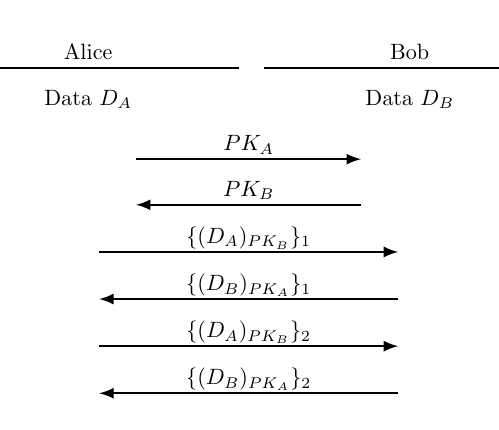
\begin{tikzpicture}[thick,scale=0.8, every node/.style={scale=0.8}]
\matrix (m)[matrix of nodes, column sep=0.5cm,row sep=6mm, nodes={draw=none, anchor=center,text depth=0pt} ]{
Alice & & Bob\\[-4mm]
Data $D_A$ & & Data $D_B$ \\[-4mm]
 & $PK_A$& \\[-4mm]
 & $PK_B$& \\[-4mm]
 & $\{(D_A)_{PK_B}\}_1$& \\[-4mm]
 & $\{(D_B)_{PK_A}\}_1$& \\[-4mm]
 & $\{(D_A)_{PK_B}\}_2$& \\[-4mm]
 & $\{(D_B)_{PK_A}\}_2$& \\[-4mm]
};

\draw[shorten <=-1.5cm,shorten >=-1.5cm] (m-1-1.south east)--(m-1-1.south west);
\draw[shorten <=-1.5cm,shorten >=-1.5cm] (m-1-3.south east)--(m-1-3.south west);

\draw[shorten <=-1cm,shorten >=-1cm,-latex] (m-3-2.south west)--(m-3-2.south east);
\draw[shorten <=-1cm,shorten >=-1cm,-latex] (m-4-2.south east)--(m-4-2.south west);
\draw[shorten <=-1cm,shorten >=-1cm,-latex] (m-5-2.south west)--(m-5-2.south east);
\draw[shorten <=-1cm,shorten >=-1cm,-latex] (m-6-2.south east)--(m-6-2.south west);
\draw[shorten <=-1cm,shorten >=-1cm,-latex] (m-7-2.south west)--(m-7-2.south east);
\draw[shorten <=-1cm,shorten >=-1cm,-latex] (m-8-2.south east)--(m-8-2.south west);

\end{tikzpicture}
\end{center}

The strength of this protocol basically lies on encryption algorithms with which the attacker cannot decrypt the received halves of encrypted messages. In case of that the attacker intentionally send some new messages to destroy the communication, he will be revealed. 

\subsubsection{Maher Manual Authentication}

In 1993, Maher got his patent for several pairing methods~\cite{maher} allowing a user to share secret DH key manually. In one method, he applied a compression function to interpret DH key $g^{ab}$ into 4-digit number. The number than is showed on each device screen. A user gets easy to compare two numbers on both devices. The protocol simply happens as follows: 
\begin{enumerate}
\item Alice and Bob generate DH value $g^a$ and $g^b$ respectively. 
\item Alice and Bob exchange their values. 
\item Both calculate $f(g^{ab})$ to 4-digit hex number, and show the result on their device's screen. 
\item The user decides accept or reject by pushing a button. 
\end{enumerate}

\begin{center}
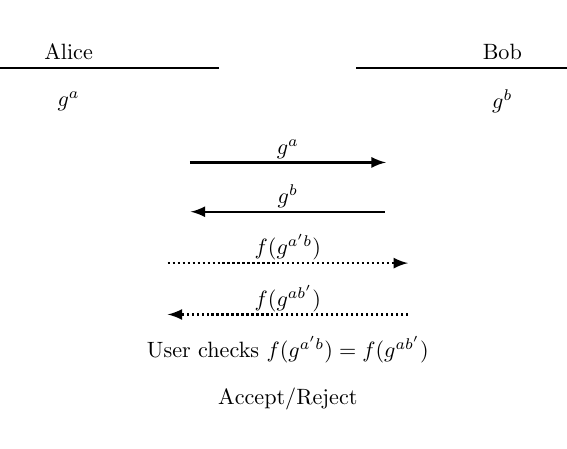
\begin{tikzpicture}[thick,scale=0.8, every node/.style={scale=0.8}]
\matrix (m)[matrix of nodes, column sep=0.5cm,row sep=6mm, nodes={draw=none, anchor=center,text depth=0pt} ]{
Alice & & Bob\\[-4mm]
$g^a$ & & $g^b$ \\[-4mm]
 & $g^a$ & \\[-4mm]
 & $g^b$ & \\[-4mm]
	&$f(g^{a'b})$ & \\ [-4mm]
	&$f(g^{ab'})$ & \\ [-4mm]
 & User checks $f(g^{a'b}) = f(g^{ab'})$ & \\ [-4mm]
 & Accept/Reject & \\ [-4mm]
};

\draw[shorten <=-1.5cm,shorten >=-1.5cm] (m-1-1.south east)--(m-1-1.south west);
\draw[shorten <=-1.5cm,shorten >=-1.5cm] (m-1-3.south east)--(m-1-3.south west);

\draw[shorten <=-1cm,shorten >=-1cm,-latex] (m-3-2.south west)--(m-3-2.south east);
\draw[shorten <=-1cm,shorten >=-1cm,-latex] (m-4-2.south east)--(m-4-2.south west);
\draw[shorten <=-1cm,shorten >=-1cm,-latex,densely dotted] (m-5-2.south west)--(m-5-2.south east);
\draw[shorten <=-1cm,shorten >=-1cm,-latex,densely dotted] (m-6-2.south east)--(m-6-2.south west);
\end{tikzpicture}
\end{center}

The protocol requires at least 80 bits over an out-of-band channel to get enough secure. At a result, this length of bit string is over-weighted on any out-of-band channel. 
 
\subsubsection{Talking to Strangers}

Balfanz et al. proposed a new scheme in \cite{Smetters02talkingto} using audio, or infrared channels to transmit a hash of public keys which is considered as a fingerprinting or digest value. The protocol works as follows:
\begin{enumerate}
\item Alice and Bob initially exchange their identifications and a hash of their pubic keys over an out-of-band channel.
\item Both sides exchange their ID and their public key on insecure channel. 
\end{enumerate}

\begin{center}
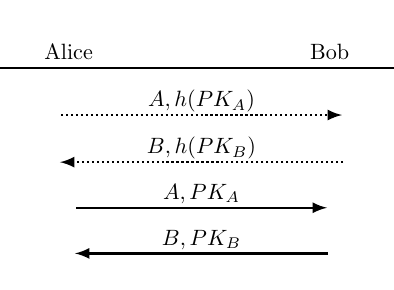
\begin{tikzpicture}[thick,scale=0.8, every node/.style={scale=0.8}]
\matrix (m)[matrix of nodes, column sep=0.5cm,row sep=6mm, nodes={draw=none, anchor=center,text depth=0pt} ]{
Alice & & Bob\\[-4mm]
 & $A,h(PK_A)$ & \\[-4mm]
 & $B,h(PK_B)$ & \\[-4mm]
 & $A,PK_A$ & \\[-4mm]
 & $B,PK_B$ & \\[-4mm]
};

\draw[shorten <=-1.5cm,shorten >=-1.5cm] (m-1-1.south east)--(m-1-1.south west);
\draw[shorten <=-1.5cm,shorten >=-1.5cm] (m-1-3.south east)--(m-1-3.south west);

\draw[shorten <=-1cm,shorten >=-1cm,-latex,densely dotted] (m-2-2.south west)--(m-2-2.south east);
\draw[shorten <=-1cm,shorten >=-1cm,-latex,densely dotted] (m-3-2.south east)--(m-3-2.south west);
\draw[shorten <=-1cm,shorten >=-1cm,-latex] (m-4-2.south west)--(m-4-2.south east);
\draw[shorten <=-1cm,shorten >=-1cm,-latex] (m-5-2.south east)--(m-5-2.south west);
\end{tikzpicture}
\end{center}

Security of this protocol mainly depends on security properties of out-of-band channels and the hash function. To prevent MITM attack, this protocol needs at least 80 bits information over each direction of OOB channel. Otherwise, the attacker can find out the pair of public keys $PK'_A/PK'_B$ in which $h(PK_A) = h(PK'_A)$ and $h(PK_B) = h(PK'_B)$ to launches a MITM attack.

\subsubsection{Visual authentication based on Integrity Checking}

Saxena et al in \cite{1624021} proposed a new pairing protocol, namely Visual authentication based on Integrity Checking(VIC) which works as follows:

\begin{enumerate}
\item Alice and Bob initially exchange their pubic keys.
\item Alice hashes both keys, and sends the hashing value to Bob. 
\item After verification the Alice's hashsing value, Bob informs Accept or Reject back to Alice. 
\end{enumerate}

\begin{center}
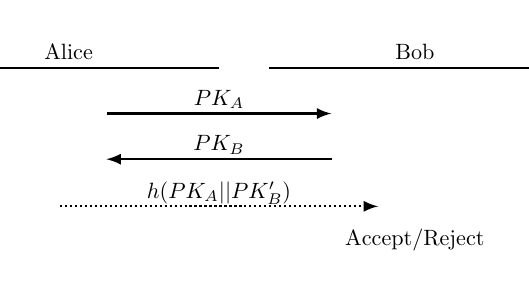
\begin{tikzpicture}[thick,scale=0.8, every node/.style={scale=0.8}]
\matrix (m)[matrix of nodes, column sep=0.5cm,row sep=6mm, nodes={draw=none, anchor=center,text depth=0pt} ]{
Alice & & Bob\\[-4mm]
 & $PK_A$ & \\[-4mm]
 & $PK_B$ & \\[-4mm]
 & $h(PK_A||PK'_B)$ & \\[-4mm]
 & & Accept/Reject \\[-4mm]
};

\draw[shorten <=-1.5cm,shorten >=-1.5cm] (m-1-1.south east)--(m-1-1.south west);
\draw[shorten <=-1.5cm,shorten >=-1.5cm] (m-1-3.south east)--(m-1-3.south west);

\draw[shorten <=-1cm,shorten >=-1cm,-latex] (m-2-2.south west)--(m-2-2.south east);
\draw[shorten <=-1cm,shorten >=-1cm,-latex] (m-3-2.south east)--(m-3-2.south west);
\draw[shorten <=-1cm,shorten >=-1cm,-latex,densely dotted] (m-4-2.south west)--(m-4-2.south east);
\end{tikzpicture}
\end{center}

Security of VIC heavily depends on strength of the hash function and requires at least 80 bits on each OOB channel to prevent hash collision. 
 
\subsubsection{Manual Authentication(MANA) Protocols}

Due to the long length of OOB messages in~\cite{1624021}, and \cite{Smetters02talkingto}, some studies tried to truncate this length into 16 or 32 bits (4 or 8 hexadecimal digits, respectively), this could lead to security weakness. Adversaries probably recover the messages from the hash-codes. To overcome this problem, Christian Gehramann and Chirs J.Michell \cite{Mitchell:2004p25948} proposed three type of manual authentication protocols: MANA I for Output-Input, MANA II for Output-Output, and MANA III for Input-Input. These protocols remarkably reduce bandwidth of OOB channel to k bits (16-20 bits) in each way while a MITM attack success probability is still hold at $2^{-k}$. 

\subsubsection*{MANA I protocol}

The authors presented a first example scheme \cite{Mitchell:2004p25948}, which is designed for situation in which one device has a keyboard, the other has a display. Although the scheme uses keyed check-function with short check-value (16 to 20 bits), it is proved to provide sufficient secure. 

\begin{enumerate}
\item $Alice$ sends a message $M$ to $Bob$ over an insecure channel. 
\item $Alice$ generates a random key $K$(16-20) bits. $Alice$ also generates $m_K(M)$, then output to its display.
\item User enters $m_K(M)$ and $K$ to $Bob$.
\item $Bob$ uses $K$ and recomputes $m_K(M)$, then compares the value that the user has entered.
\item The user copies success or failure. 
\end{enumerate}

\begin{center}
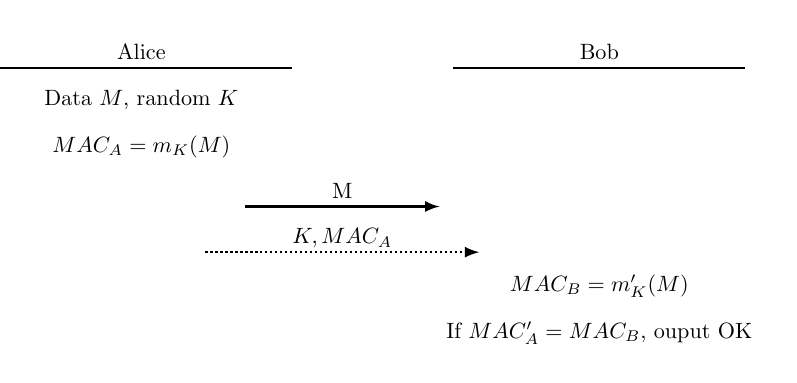
\begin{tikzpicture}[thick,scale=0.8, every node/.style={scale=0.8}]
\matrix (m)[matrix of nodes, column sep=0.5cm,row sep=6mm, nodes={draw=none, anchor=center,text depth=0pt} ]{
Alice & & Bob\\[-4mm]
Data $M$, random $K$ & &  \\[-4mm]
$MAC_A = m_K(M)$ & & \\ [-4mm]
				&M& \\ [-4mm]
				&$K,MAC_A$ & \\ [-4mm]
& & $MAC_B = m_K'(M)$ \\ [-4mm]
& & If $MAC'_A = MAC_B$, ouput OK \\ [-4mm]
};

\draw[shorten <=-1.5cm,shorten >=-1.5cm] (m-1-1.south east)--(m-1-1.south west);
\draw[shorten <=-1.5cm,shorten >=-1.5cm] (m-1-3.south east)--(m-1-3.south west);

\draw[shorten <=-1cm,shorten >=-1cm,-latex] (m-4-2.south west)--(m-4-2.south east);
\draw[shorten <=-1cm,shorten >=-1cm,-latex,densely dotted] (m-5-2.south west)--(m-5-2.south east);
\end{tikzpicture}
\end{center}

\subsubsection*{MANA II protocol}

MANA II \cite{Mana2} is a variant of MANA I. In this scheme, both devices are equipped with displays and keyboards. The protocol works as follows: 

\begin{enumerate}
\item $Alice$ sends a message $M$ to $Bob$ over an insecure channel. 
\item $Alice$ generates a random key $K_A$(16-20) bits. $Alice$ also generates $m_{K_A}(M)$, then output it to the user over a secured channel. 
\item $Alice$ sends key $K_A$ to $Bob$ over the insecure channel. 
\item $Bob$ uses $K_A$ and recomputes $m_{K_A}(M)$, then sends $m_{K_A}(M)$ to the user. 
\item The user compares two values from both devices. Then if results are matched, the user indicates success to both devices over a secured channel. 
\end{enumerate}

\begin{center}
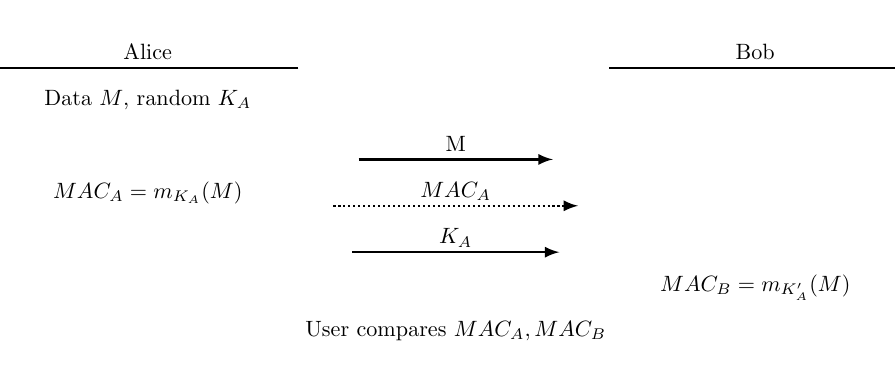
\begin{tikzpicture}[thick,scale=0.8, every node/.style={scale=0.8}]
\matrix (m)[matrix of nodes, column sep=0.5cm,row sep=6mm, nodes={draw=none, anchor=center,text depth=0pt} ]{
Alice & & Bob\\[-4mm]
Data $M$, random $K_A$ & & \\[-4mm]
& M & \\ [-4mm]
$MAC_A = m_{K_A}(M)$ & $MAC_A$ &\\[- 4mm]
& $K_A$ & \\ [-4mm]
& & $MAC_B = m_{K'_A}(M)$ \\[-4mm]
&User compares $MAC_A, MAC_B$ & \\ [-4mm]
};


\draw[shorten <=-1.5cm,shorten >=-1.5cm] (m-1-1.south east)--(m-1-1.south west);
\draw[shorten <=-1.5cm,shorten >=-1.5cm] (m-1-3.south east)--(m-1-3.south west);

\draw[shorten <=-1cm,shorten >=-1cm,-latex] (m-3-2.south west)--(m-3-2.south east);
\draw[shorten <=-1cm,shorten >=-1cm,-latex,densely dotted] (m-4-2.south west)--(m-4-2.south east);
\draw[shorten <=-1cm,shorten >=-1cm,-latex] (m-5-2.south west)--(m-5-2.south east);
\end{tikzpicture}
\end{center}


\subsubsection*{MANA III protocol}

MANA III protocol~\cite{Mitchell:2004p25948} is designed for a situation in which both devices have keyboards. Both devices are assumed on agreement on a public data $M$. Here, $m_K(M)$ denotes a MAC value computed using a key $K$ and a data string $M$. $I_A$ and $I_B$ are identifications of $Alice$ and $Bob$, respectively. The scheme operates as follows. 

\begin{enumerate}
\item $Alice$ sends a message $M$ to $Bob$ over an insecure channel. 
\item A user generates a short random bit-string (16-20) bits $R$ and enters it to 2 devices.
\item $Alice$ generates a key $K_A$, computes $MAC_A = m_{K_A}(ID_A,M,R)$, then sends $MAC_A$ to $Bob$ over a wireless link.
\item $Bob$ generates a key $K_B$, computes $MAC_B = m_{K_B}(ID_B,M,R)$, then sends $MAC_B$ to $Alice$ over the wireless link.
\item When $Alice$ receives $MAC_B$, then sends $K_A$ to $Bob$ over a secured channel.
\item When $Bob$ receives $MAC_A$, then sends $K_B$ to $Alice$ over the secured channel.
\item $Alice$ recomputes $MAC_B$ and verifies its stored value of $M$, the expected identifier $I_B$, and random value $R$.
\item $Bob$ recomputes $MAC_A$ and verifies its stored value of $M$, the expected identifier$I_A$, and random $R$.
\item If(and only if) both devices indicate success, the user indicates success two both devices.
\end{enumerate}


\begin{center}
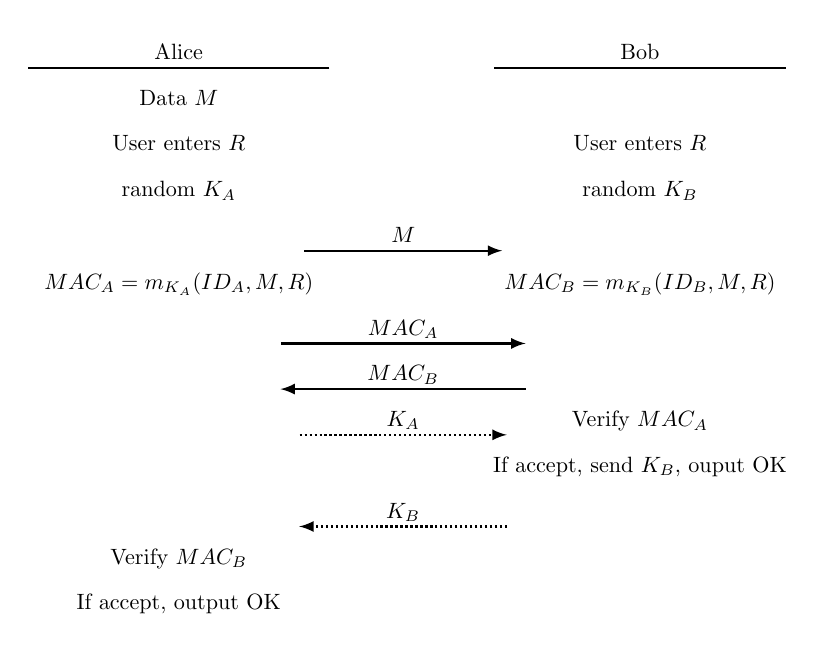
\begin{tikzpicture}[thick,scale=0.8, every node/.style={scale=0.8}]
\matrix (m)[matrix of nodes, column sep=0.5cm,row sep=6mm, nodes={draw=none, anchor=center,text depth=0pt} ]{
Alice & & Bob\\[-4mm]
Data $M$ & &  \\[-4mm]
User enters $R$ & & User enters $R$ \\[-4mm]
random $K_A$ & & random $K_B$\\[- 4mm]
& $M$ & \\ [-4mm]

$MAC_A = m_{K_A}(ID_A,M,R)$ & & $MAC_B = m_{K_B}(ID_B,M,R)$ \\[- 4mm]

& $MAC_A$ & \\ [-4mm]
& $MAC_B$ & \\ [-4mm]
& $K_A$ & Verify $MAC_A$ \\ [-4mm]
& & If accept, send $K_B$, ouput OK \\ [-4mm]
& $K_B$ & \\ [-4mm]
Verify $MAC_B$& & \\ [-4mm]
If accept, output OK & & \\ [-4mm]
};

\draw[shorten <=-1.5cm,shorten >=-1.5cm] (m-1-1.south east)--(m-1-1.south west);
\draw[shorten <=-1.5cm,shorten >=-1.5cm] (m-1-3.south east)--(m-1-3.south west);

\draw[shorten <=-1cm,shorten >=-1cm,-latex] (m-5-2.south west)--(m-5-2.south east);
\draw[shorten <=-1cm,shorten >=-1cm,-latex] (m-7-2.south west)--(m-7-2.south east);
\draw[shorten <=-1cm,shorten >=-1cm,-latex] (m-8-2.south east)--(m-8-2.south west);
\draw[shorten <=-1cm,shorten >=-1cm,-latex,densely dotted] (m-9-2.south west)--(m-9-2.south east);
\draw[shorten <=-1cm,shorten >=-1cm,-latex,densely dotted] (m-11-2.south east)--(m-11-2.south west);
\end{tikzpicture}
\end{center}

\subsubsection*{Analysis of MANA Protocols}

An out-of-band channel used in MANA I and II could be a public or protected channel, while MANA III strongly requires a private channel as the key $R$ must be confident. If leaking $R$, MANA III protocol is definitely a victim of MITM attack. Furthermore, success probability of attacks in MANA protocol is $2^{-k}$ where $k$ is length of check-value messages in MANA I and MANA II, and is the length of $R$ in MANA III. In term of optimisation, in MANA I and II, the user must compares check-values and the key $K$. However, in term of security, MANA I may provide a stronger security level than others. 

\subsubsection{Ephemeral Pairing Protocols}
\subsubsection*{Hoepman AKA Protocol}

Jaap-Henk Hoepman in \cite{Hoepman:2004aa} proposed his protocols by exploited out-of-band channel properties. In his protocol, parties securely share their DH public keys in two phases. First, long hashes of both sides' public keys are exchanged over insecure channels. Second, short hashes are sent over out-of-band channels. The detail protocol is illustrated as follows.

\begin{enumerate}
\item Alice and Bob generate DH-value $g^a$ and $g^b$ respectively. 
\item Both sides exchange a long hashing value of $g^a$ and $g^b$ over an insecure channel. 
\item After the reception of the long hashing value, both sides calculate a short hashing value of $g^a$ and $g^b$, exchange them over an out-of-band channel. 
\item At the end, both sides reveal their value $g^a$ and $g^b$ to each other in the insecure channel. 
\end{enumerate}

\begin{center}
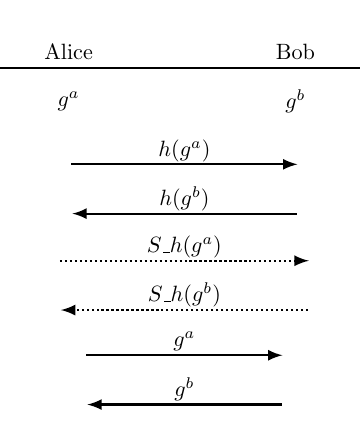
\begin{tikzpicture}[thick,scale=0.8, every node/.style={scale=0.8}]
\matrix (m)[matrix of nodes, column sep=0.5cm,row sep=6mm, nodes={draw=none, anchor=center,text depth=0pt} ]{
Alice & & Bob\\[-4mm]
$g^a$ & & $g^b$\\[-4mm]
& $h(g^a)$ & \\[-4mm]
& $h(g^b)$ & \\[-4mm]
& $S\_h(g^a)$ & \\[-4mm]
& $S\_h(g^b)$ & \\[-4mm]
& $g^a$ & \\[-4mm]
& $g^b$ & \\[-4mm]
};

\draw[shorten <=-1.5cm,shorten >=-1.5cm] (m-1-1.south east)--(m-1-1.south west);
\draw[shorten <=-1.5cm,shorten >=-1.5cm] (m-1-3.south east)--(m-1-3.south west);

\draw[shorten <=-1cm,shorten >=-1cm,-latex] (m-3-2.south west)--(m-3-2.south east);
\draw[shorten <=-1cm,shorten >=-1cm,-latex] (m-4-2.south east)--(m-4-2.south west);
\draw[shorten <=-1cm,shorten >=-1cm,-latex,densely dotted] (m-5-2.south west)--(m-5-2.south east);
\draw[shorten <=-1cm,shorten >=-1cm,-latex,densely dotted] (m-6-2.south east)--(m-6-2.south west);
\draw[shorten <=-1cm,shorten >=-1cm,-latex] (m-7-2.south west)--(m-7-2.south east);
\draw[shorten <=-1cm,shorten >=-1cm,-latex] (m-8-2.south east)--(m-8-2.south west);

\end{tikzpicture}
\end{center}

\subsubsection*{Improved Ephemeral Pairing}

Nguyen and Roscoe~\cite{Nguyen09authenticationprotocols} proposed an improved version of Hoepman protocol by cutting off one message on OOB channel. The protocol works as follows:
\begin{enumerate}
\item Alice and Bob generate DH-value $g^a$ and $g^b$ respectively. 
\item Alice sends $h(A,g^a)$ to Bob. 
\item Both sides exchange $g^a$ and $g^b$ to each other. 
\item At the end, Alice calculates a short hash of $g^a \oplus g'^b$, then sends it to Bob over an out-of-band channel. 
\end{enumerate}

\begin{center}
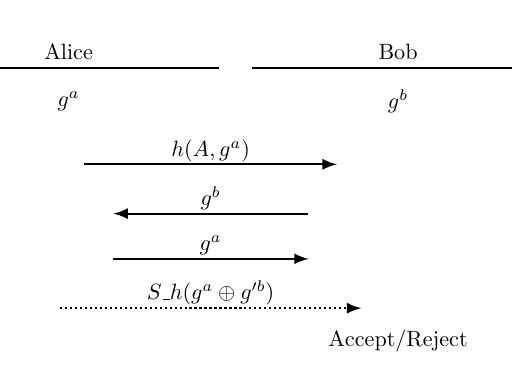
\begin{tikzpicture}[thick,scale=0.8, every node/.style={scale=0.8}]
\matrix (m)[matrix of nodes, column sep=0.5cm,row sep=6mm, nodes={draw=none, anchor=center,text depth=0pt} ]{
Alice & & Bob\\[-4mm]
$g^a$ & & $g^b$\\[-4mm]
& $h(A,g^a)$ & \\[-4mm]
& $g^b$ & \\[-4mm]
& $g^a$ & \\[-4mm]
& $S\_h(g^a\oplus g'^b)$ & \\[-4mm]
& & Accept/Reject \\[-4mm]
};

\draw[shorten <=-1.5cm,shorten >=-1.5cm] (m-1-1.south east)--(m-1-1.south west);
\draw[shorten <=-1.5cm,shorten >=-1.5cm] (m-1-3.south east)--(m-1-3.south west);

\draw[shorten <=-1cm,shorten >=-1cm,-latex] (m-3-2.south west)--(m-3-2.south east);
\draw[shorten <=-1cm,shorten >=-1cm,-latex] (m-4-2.south east)--(m-4-2.south west);
\draw[shorten <=-1cm,shorten >=-1cm,-latex] (m-5-2.south west)--(m-5-2.south east);
\draw[shorten <=-1cm,shorten >=-1cm,-latex,densely dotted] (m-6-2.south west)--(m-6-2.south east);


\end{tikzpicture}
\end{center}

\subsubsection*{Analysis of Ephemeral Protocols}

Security of Hoepman protocol heavily depends on freshness of DH public keys in each protocol session. Otherwise, an attacker is able to discover a matching key with the same short hash output, then successfully launches a MITM attack. Hoepman also provided a proof of his protocol in the Bellare-Pointcheval- Rogaway model. The improvement scheme of Nguyen and Roscoe remains the same requirement. 

\subsubsection{Wong-Stajano Multichanel Security Protocols}\label{WS}

Wong and Stajano~\cite{10.1109/MPRV.2007.76} proposed new mutual authentication and key agreement protocols over bidirectional and unidirectional public out-of-band channels. Their protocols exploit a short authenticated string over visual channels which provide data origin authenticity. 

\subsubsection*{Protocol with Bidirectional Channel}

Wong and Stajano introduced a new variant of MANA III protocol which works as follows:

\begin{enumerate}
\item Alice generates a random number $r_a$, a key $K_A$, and DH-value $g^a$.
\item Bob generates a random number $r_b$, a key $K_B$, and DH-value $g^b$.
\item Both sides exchange $g^a$ and $g^b$ to each other.
\item Alice calculates $MAC_{K_A}(A,g^a,g'^b,r_a,K_A)$, then sends it to Bob. 
\item Bob calculates $MAC_{K_B}(B,g^b,g'^a,r_b,K_B)$, then sends it to Alice.
\item Both sides exchange their $r_a$ and $r_b$ to each other over an out-of-band channel. 
\item At the end, Bob sides exchange their $K_A$ and $K_B$ to each other. 
\end{enumerate}

\begin{center}
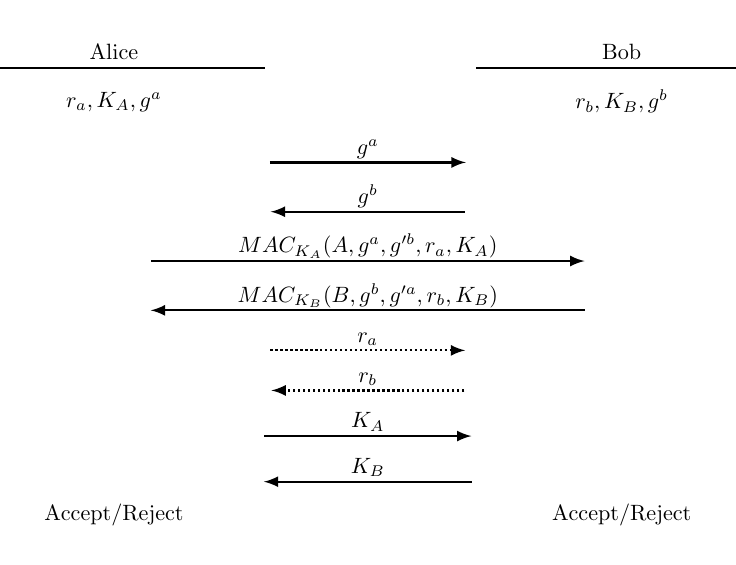
\begin{tikzpicture}[thick,scale=0.8, every node/.style={scale=0.8}]
\matrix (m)[matrix of nodes, column sep=0.5cm,row sep=6mm, nodes={draw=none, anchor=center,text depth=0pt} ]{
Alice & & Bob\\[-4mm]
$r_a,K_A,g^a$ & & $r_b,K_B,g^b$ \\[-4mm]
& $g^a$ & \\[-4mm]
& $g^b$ & \\[-4mm]
& $ MAC_{K_A}(A,g^a,g'^b,r_a,K_A)$ & \\[-4mm]
& $ MAC_{K_B}(B,g^b,g'^a,r_b,K_B)$ & \\[-4mm]
& $r_a$ & \\[-4mm]
& $r_b$ & \\[-4mm]
& $K_A$ & \\[-4mm]
& $K_B$ & \\[-4mm]
Accept/Reject & & Accept/Reject \\[-4mm]
};

\draw[shorten <=-1.5cm,shorten >=-1.5cm] (m-1-1.south east)--(m-1-1.south west);
\draw[shorten <=-1.5cm,shorten >=-1.5cm] (m-1-3.south east)--(m-1-3.south west);

\draw[shorten <=-1cm,shorten >=-1cm,-latex] (m-3-2.south west)--(m-3-2.south east);
\draw[shorten <=-1cm,shorten >=-1cm,-latex] (m-4-2.south east)--(m-4-2.south west);
\draw[shorten <=-1cm,shorten >=-1cm,-latex] (m-5-2.south west)--(m-5-2.south east);
\draw[shorten <=-1cm,shorten >=-1cm,-latex] (m-6-2.south east)--(m-6-2.south west);
\draw[shorten <=-1cm,shorten >=-1cm,-latex,densely dotted] (m-7-2.south west)--(m-7-2.south east);
\draw[shorten <=-1cm,shorten >=-1cm,-latex,densely dotted] (m-8-2.south east)--(m-8-2.south west);
\draw[shorten <=-1cm,shorten >=-1cm,-latex] (m-9-2.south west)--(m-9-2.south east);
\draw[shorten <=-1cm,shorten >=-1cm,-latex] (m-10-2.south east)--(m-10-2.south west);

\end{tikzpicture}
\end{center}

In term of usability, the above protocol spends 6-move insecure communication, and long hash of DH public keys that put a heavy pressure on constrained devices. Realising this limitation, the authors improved their first work by an improved version over the bidirectional public out-of-band channel. The new protocol works as follows:

\begin{enumerate}
\item Alice generates a random number $r_a$, a key $K_A$, and DH-value $g^a$.
\item Bob generates a random number $r_b$, a key $K_B$, and DH-value $g^b$.
\item Alice calculates $MAC_{K_A}(A,g^a,g'^b,r_a,K_A)$, then sends it with Alice's identification $A$ and $g^a$ to Bob. 
\item Bob calculates $MAC_{K_B}(B,g^b,g'^a,r_b,K_B)$, then sends it with Bob's identification $B$ and $g^b$ to Alice.
\item Both sides exchange their $r_a$ and $r_b$ to each other over an out-of-band channel. 
\item At the end, Bob sides exchange their $K_A$ and $K_B$ to each other. 
\item Alice informs to Bob Accept or Reject the session.
\end{enumerate}

\begin{center}
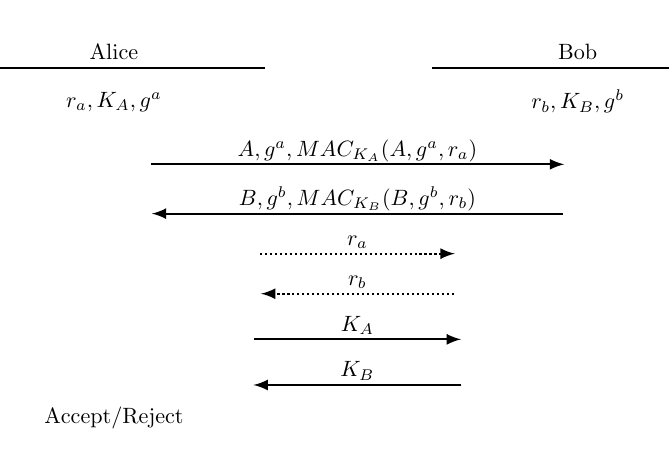
\begin{tikzpicture}[thick,scale=0.8, every node/.style={scale=0.8}]
\matrix (m)[matrix of nodes, column sep=0.5cm,row sep=6mm, nodes={draw=none, anchor=center,text depth=0pt} ]{
Alice & & Bob\\[-4mm]
$r_a,K_A,g^a$ & & $r_b,K_B,g^b$ \\[-4mm]
& $A, g^a, MAC_{K_A}(A,g^a,r_a)$ & \\[-4mm]
& $B, g^b, MAC_{K_B}(B,g^b,r_b)$ & \\[-4mm]
& $r_a$ & \\[-4mm]
& $r_b$ & \\[-4mm]
& $K_A$ & \\[-4mm]
& $K_B$ & \\[-4mm]
Accept/Reject & & \\[-4mm]
};

\draw[shorten <=-1.5cm,shorten >=-1.5cm] (m-1-1.south east)--(m-1-1.south west);
\draw[shorten <=-1.5cm,shorten >=-1.5cm] (m-1-3.south east)--(m-1-3.south west);

\draw[shorten <=-1cm,shorten >=-1cm,-latex] (m-3-2.south west)--(m-3-2.south east);
\draw[shorten <=-1cm,shorten >=-1cm,-latex] (m-4-2.south east)--(m-4-2.south west);
\draw[shorten <=-1cm,shorten >=-1cm,-latex,densely dotted] (m-5-2.south west)--(m-5-2.south east);
\draw[shorten <=-1cm,shorten >=-1cm,-latex,densely dotted] (m-6-2.south east)--(m-6-2.south west);
\draw[shorten <=-1cm,shorten >=-1cm,-latex] (m-7-2.south west)--(m-7-2.south east);
\draw[shorten <=-1cm,shorten >=-1cm,-latex] (m-8-2.south east)--(m-8-2.south west);

\end{tikzpicture}
\end{center}

The improved protocol combines the first 4 messages of MANA III variant to 2 messages, and uses the MAC function, instead of a general hash function. 
 
\subsubsection*{Protocol with Unidirectional Channel}

In the same paper, Wong and Stajano also proposed a new protocol with unidirectional out-of-band channel. This version only spend 3 move on the wireless channel rather than 4-move in bidirectional version. The protocol works as follows:
\begin{enumerate}
\item Alice generates a random number $r_a$ and DH-value $g^a$.
\item Bob generates a random number $r_b$, a key $K_B$, and DH-value $g^b$.
\item Alice sends $g^a$ to Bob. 
\item Bob calculates $MAC_{K_B}(B,g^b,g'^a,r_b,K_B)$, then sends it with Bob's identification $B$ and $g^b$ to Alice.
\item Alice informs to Bob that she has already received his message over an out-of-band channel. 
\item Bob sends $r_b$ to Alice over the out-of-band channel. 
\item Bob sends $K_B$ to Alice. 
\item Alice informs to Bob Accept or Reject the session.
\end{enumerate}

\begin{center}
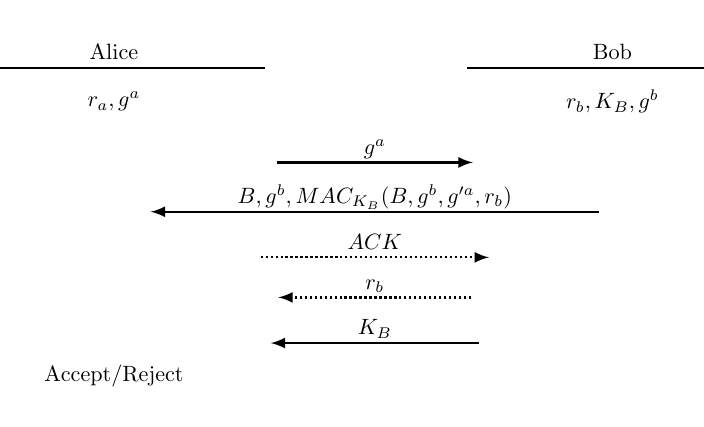
\begin{tikzpicture}[thick,scale=0.8, every node/.style={scale=0.8}]
\matrix (m)[matrix of nodes, column sep=0.5cm,row sep=6mm, nodes={draw=none, anchor=center,text depth=0pt} ]{
Alice & & Bob\\[-4mm]
$r_a,g^a$ & & $r_b,K_B,g^b$ \\[-4mm]
& $g^a$ & \\[-4mm]
& $B, g^b, MAC_{K_B}(B,g^b,g'^a,r_b)$ & \\[-4mm]
& $ACK$ & \\[-4mm]
& $r_b$ & \\[-4mm]
& $K_B$ & \\[-4mm]
Accept/Reject & & \\[-4mm]
};

\draw[shorten <=-1.5cm,shorten >=-1.5cm] (m-1-1.south east)--(m-1-1.south west);
\draw[shorten <=-1.5cm,shorten >=-1.5cm] (m-1-3.south east)--(m-1-3.south west);

\draw[shorten <=-1cm,shorten >=-1cm,-latex] (m-3-2.south west)--(m-3-2.south east);
\draw[shorten <=-1cm,shorten >=-1cm,-latex] (m-4-2.south east)--(m-4-2.south west);
\draw[shorten <=-1cm,shorten >=-1cm,-latex,densely dotted] (m-5-2.south west)--(m-5-2.south east);
\draw[shorten <=-1cm,shorten >=-1cm,-latex,densely dotted] (m-6-2.south east)--(m-6-2.south west);
\draw[shorten <=-1cm,shorten >=-1cm,-latex] (m-7-2.south east)--(m-7-2.south west);

\end{tikzpicture}
\end{center}

In term of efficiency, this unidirectional protocol only spends 5 messages including 2 out-of-band messages, that decreases both computation and communication cost compared to costs of two previous protocols. 
\subsubsection*{Improved Wong-Stajano Key Agreement Protocol}

Nguyen and Roscoe~\cite{Nguyen09authenticationprotocols} proposed an variant of Wong-Stajano protocol. The new scheme cuts off long keys, and replaces two different authenticated string $r_a$ and $r_b$ by a single value $r_a\oplus r'_b$. The protocol works as follows:
\begin{enumerate}
\item Alice generates a random number $r_a$ and DH-value $g^a$.
\item Bob generates a random number $r_b$, and DH-value $g^b$.
\item Alice calculates $h(A,g^a,r_a)$, and sends it to Bob. 
\item Bob calculates $h(B,g^b,r_b)$, then sends it to Alice.
\item Alice sends $r_a$ and $g^a$ to Bob. 
\item Bob sends $r_b$ and $g^b$ to Alice. 
\item Alice calculates $r_a\oplus r'_b$, then pushes it on an out-of-band channel to Bob. 
\item Bob informs to Alice Accept or Reject the session.
\end{enumerate}

\begin{center}
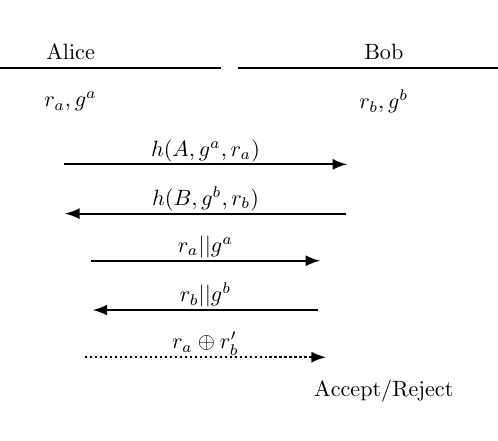
\begin{tikzpicture}[thick,scale=0.8, every node/.style={scale=0.8}]
\matrix (m)[matrix of nodes, column sep=0.5cm,row sep=6mm, nodes={draw=none, anchor=center,text depth=0pt} ]{
Alice & & Bob\\[-4mm]
$r_a,g^a$ & & $r_b,g^b$ \\[-4mm]
& $h(A,g^a,r_a)$ & \\[-4mm]
& $h(B,g^b,r_b)$ & \\[-4mm]
& $r_a||g^a$ & \\[-4mm]
& $r_b||g^b$ & \\[-4mm]
& $r_a\oplus r'_b$ & \\[-4mm]
& & Accept/Reject \\[-4mm]
};

\draw[shorten <=-1.5cm,shorten >=-1.5cm] (m-1-1.south east)--(m-1-1.south west);
\draw[shorten <=-1.5cm,shorten >=-1.5cm] (m-1-3.south east)--(m-1-3.south west);

\draw[shorten <=-1cm,shorten >=-1cm,-latex] (m-3-2.south west)--(m-3-2.south east);
\draw[shorten <=-1cm,shorten >=-1cm,-latex] (m-4-2.south east)--(m-4-2.south west);
\draw[shorten <=-1cm,shorten >=-1cm,-latex] (m-5-2.south west)--(m-5-2.south east);
\draw[shorten <=-1cm,shorten >=-1cm,-latex] (m-6-2.south east)--(m-6-2.south west);
\draw[shorten <=-1cm,shorten >=-1cm,-latex,densely dotted] (m-7-2.south west)--(m-7-2.south east);

\end{tikzpicture}
\end{center}

\subsubsection*{Analysis of Wong-Stajano Protocols}

Wong-Stajano protocols were designed against either passive or active attacks. Passive attacks are resisted by DH components, while active attacks are resisted by short hash values over OOB channel. However, our work has successfully exploited the protocols. The counterexample will be presented in the following section. 

\subsubsection{Short Authenticated String-Based Authentication Key Agreement Protocols}

MANA-based protocol family usually requires a strong assumption on a channel on which adversaries are not able to delay or relay any OOB message. To ease this strict condition, Serge Vaudenay introduced a protocol~\cite{Vaudenay:2005qa} based on Short Authentication String (SAS) in 2005. This scheme uses k-bit on OOB channel, and still preserves $2^{-k}$ attack success probability.

\subsubsection*{4-Move SAS-based Mutual-Authentication}

Vaudenay presented his first authentication protocol based on a short authenticated string over an OOB channel~\cite{Vaudenay:2005qa}. The protocol is illustrated as follows.

\begin{enumerate}
\item Alice types a message $M_A$, then picks a random value $r_a$. Bob types a message $M_B$, then picks a random value $r_b$
\item Alice computes $(c_A||d_A) \leftarrow Commit(0||M_A||r_a)$, and sends $M_A, c_A$ to Bob.
\item Bob computes $(c_B||d_B) \leftarrow Commit(0||M_B||r_b)$ sends $M_B, c_B$ to Alice.
\item Alice sends $d_A$ to Bob. Then Bob computes $r'_a \leftarrow Open(0||M_A,c'_A,d'_A)$. 
\item Bob sends $d_B$ to Alice. Then Alice computes $r'_b \leftarrow Open(0||M_B,c'_B,d'_B)$. 
\item Alice computes $SAS_A \leftarrow r_a \oplus r'_b$, and sends $SAS$ to Bob over an out-of-band channel. 
\item Bob computes $SAS_B = r'_a \oplus r_b$, then sends $SAS_B$ back to Alice over his out-of-band channel. 
\item Both sides compare their calculated SAS value to received one from the other. 
\end{enumerate}

\begin{center}
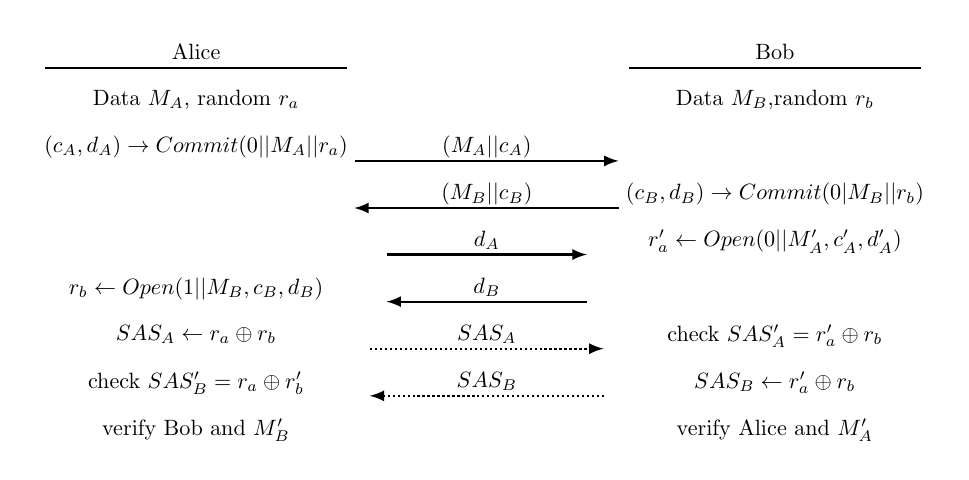
\begin{tikzpicture}[thick,scale=0.8, every node/.style={scale=0.8}]
\matrix (m)[matrix of nodes, column sep=1cm,row sep=6mm, nodes={draw=none, anchor=center,text depth=0pt} ]{
Alice & & Bob\\[-4mm]
Data $M_A$, random $r_a$ & & Data $M_B$,random $r_b$ \\[-4mm]
$(c_A,d_A)\rightarrow Commit(0||M_A||r_a)$ & $(M_A||c_A)$ & \\[- 4mm]
							 & $(M_B||c_B)$ & $(c_B,d_B)\rightarrow Commit(0|M_B||r_b)$ \\[- 4mm]	
						  & $d_A$ & $r'_a \leftarrow Open(0||M'_A,c'_A,d'_A)$ \\[-4mm]
$r_b \leftarrow Open(1||M_B,c_B,d_B)$ & $d_B$ & \\[-4mm]
$SAS_A \leftarrow r_a\oplus r_b $ & $SAS_A$ & check $SAS'_A = r'_a\oplus r_b$ \\ [-4mm]
check $SAS'_B = r_a\oplus r'_b$ & $SAS_B$ & $SAS_B \leftarrow r'_a\oplus r_b $ \\ [-4mm]
verify Bob and $M'_B$ 			 & & verify Alice and $M'_A$ \\ [-4mm]
};

\draw[shorten <=-1.5cm,shorten >=-1.5cm] (m-1-1.south east)--(m-1-1.south west);
\draw[shorten <=-1.5cm,shorten >=-1.5cm] (m-1-3.south east)--(m-1-3.south west);
\draw[shorten <=-1cm,shorten >=-1cm,-latex] (m-3-2.south west)--(m-3-2.south east);
\draw[shorten <=-1cm,shorten >=-1cm,-latex] (m-4-2.south east)--(m-4-2.south west);
\draw[shorten <=-1cm,shorten >=-1cm,-latex] (m-5-2.south west)--(m-5-2.south east);
\draw[shorten <=-1cm,shorten >=-1cm,-latex] (m-6-2.south east)--(m-6-2.south west);
\draw[shorten <=-1cm,shorten >=-1cm,-latex,densely dotted] (m-7-2.south west)--(m-7-2.south east);
\draw[shorten <=-1cm,shorten >=-1cm,-latex,densely dotted] (m-8-2.south east)--(m-8-2.south west);
\end{tikzpicture}
\end{center}

\subsubsection*{3-Move SAS-based Mutual-Authentication}

Sylvain Pasini and Serge Vaudenay \cite{Pasini:2006fu} attempted to decrease interaction cost of the protocol~\cite{Vaudenay:2005qa} down to 3 moves by advantage of a random oracle model. The protocol runs as follows. 

\begin{enumerate}
\item Alice types a message $M$, then picks a random value $r_a$. Bob types a message $M$, then picks a random value $r_b$
\item Alice computes $(c||d) \leftarrow Commit(M||r_a)$, and sends $c$ to Bob.
\item Bob sends $r_b$ to Alice.
\item Alice sends $M$ to Bob. Then Bob computes $r'_a \leftarrow Open(M,c'_A,d'_A)$. 
\item Alice computes $SAS_A \leftarrow r_a \oplus r'_b$, and sends $SAS$ to Bob over an out-of-band channel. 
\item Bob computes $SAS_B = r'_a \oplus r_b$, then sends $SAS_B$ back to Alice over his out-of-band channel. 
\item Bob verifies SAS and Alice. Alice compares both values of SAS and verifies Bob. 
\end{enumerate}

\begin{center}
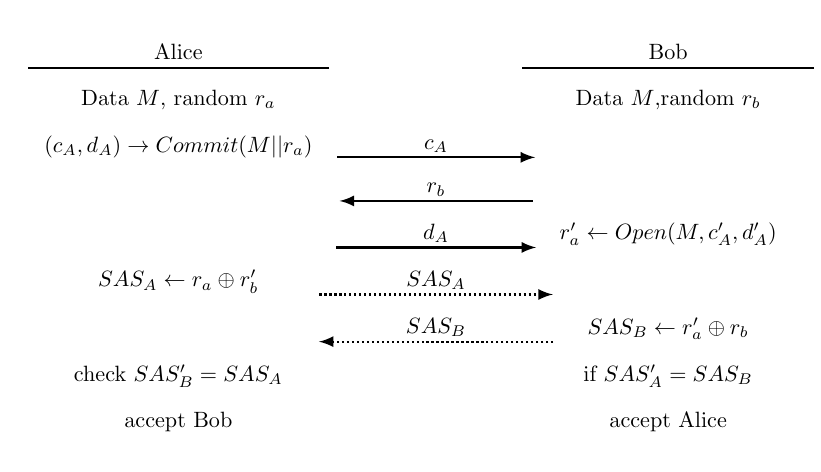
\begin{tikzpicture}[thick,scale=0.8, every node/.style={scale=0.8}]
\matrix (m)[matrix of nodes, column sep=1cm,row sep=6mm, nodes={draw=none, anchor=center,text depth=0pt} ]{
Alice & & Bob\\[-4mm]
Data $M$, random $r_a$ & & Data $M$,random $r_b$ \\[-4mm]
$(c_A,d_A)\rightarrow Commit(M||r_a)$ & $c_A$ & \\[- 4mm]
									& $r_b$ & \\[- 4mm]
									& $d_A$ & $r'_a \leftarrow Open(M,c'_A,d'_A)$ \\[-4mm]
$SAS_A \leftarrow r_a\oplus r_b' $ & $SAS_A$ & \\ [-4mm]
						 	 & $SAS_B$ & $SAS_B \leftarrow r'_a\oplus r_b$ \\ [-4mm] 
check $SAS'_B = SAS_A$ 					 & & if $SAS'_A = SAS_B$ \\ [-4mm]
accept Bob 			 & & accept Alice \\ [-4mm]
};

\draw[shorten <=-1.5cm,shorten >=-1.5cm] (m-1-1.south east)--(m-1-1.south west);
\draw[shorten <=-1.5cm,shorten >=-1.5cm] (m-1-3.south east)--(m-1-3.south west);
\draw[shorten <=-1cm,shorten >=-1cm,-latex] (m-3-2.south west)--(m-3-2.south east);
\draw[shorten <=-1cm,shorten >=-1cm,-latex] (m-4-2.south east)--(m-4-2.south west);
\draw[shorten <=-1cm,shorten >=-1cm,-latex] (m-5-2.south west)--(m-5-2.south east);
\draw[shorten <=-1cm,shorten >=-1cm,-latex,densely dotted] (m-6-2.south west)--(m-6-2.south east);
\draw[shorten <=-1cm,shorten >=-1cm,-latex,densely dotted] (m-7-2.south east)--(m-7-2.south west);
\end{tikzpicture}
\end{center}

\subsubsection*{3-Move SAS-based Cross Authentication}

New SAS-based Cross Authentication based on the previous 3-move mutual authentication protocol improves a number of exchanged messages and uses a strongly universal hash function family. The protocol is presented as follow. 
 
\begin{enumerate}
\item Alice types message $M_A$, then picks a random value $r_a$. Bob types message $M_B$, then picks a random value $r_b$
\item Alice computes $(c_A||d_A) \leftarrow Commit(0,M_A,r_a)$, and sends $(M_A,c_A)$ to Bob.
\item Bob sends $(M_B,r_b)$ to Alice.
\item Alice sends $d_A$ to Bob. Bob computes $r_a \leftarrow Open(0|M'_A,c'_A,d'_A)$. 
\item Alice computes $SAS_A \leftarrow r'_b \oplus h_{r_a}(M'_B)$, and send $SAS_A$ to Bob through out-of-band channel. 
\item Bob computes $SAS_B \leftarrow r_b \oplus h_{r'_a}(M_B)$ and send $SAS_B$ to Alice through out-of-band channel. 
\item Alice and Bob check received $SAS$ with their own $SAS$. Alice verifies Bob and $M_B$. And, Bob verifies Alice and $M_A$.
\end{enumerate}

\begin{center}
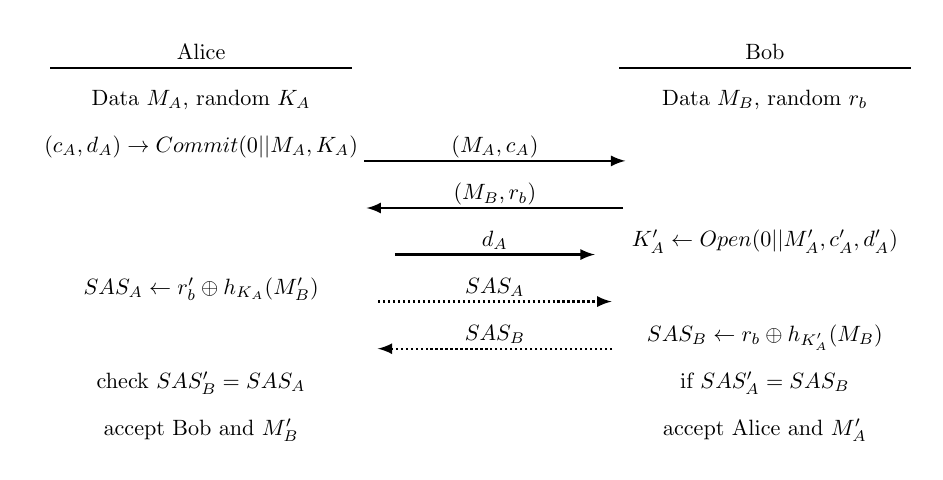
\begin{tikzpicture}[thick,scale=0.8, every node/.style={scale=0.8}]
\matrix (m)[matrix of nodes, column sep=1cm,row sep=6mm, nodes={draw=none, anchor=center,text depth=0pt} ]{
Alice & & Bob\\[-4mm]
Data $M_A$, random $K_A$ & & Data $M_B$, random $r_b$ \\[-4mm]
$(c_A,d_A)\rightarrow Commit(0||M_A,K_A)$ & $(M_A,c_A)$ & \\[- 4mm]
							 & $(M_B,r_b)$ & \\[- 4mm]	
						  & $d_A$ & $K'_A \leftarrow Open(0||M'_A,c'_A,d'_A)$ \\[-4mm]
$SAS_A \leftarrow r'_b\oplus h_{K_A}(M'_B)$ & $SAS_A$ & \\ [-4mm]
								& $SAS_B$ & $SAS_B \leftarrow r_b\oplus h_{K'_A}(M_B)$ \\ [-4mm]
check $SAS'_B = SAS_A$ 					 & & if $SAS'_A = SAS_B$ \\ [-4mm]
accept Bob and $M'_B$ 			 & & accept Alice and $M'_A$ \\ [-4mm]
};

\draw[shorten <=-1.5cm,shorten >=-1.5cm] (m-1-1.south east)--(m-1-1.south west);
\draw[shorten <=-1.5cm,shorten >=-1.5cm] (m-1-3.south east)--(m-1-3.south west);

\draw[shorten <=-1cm,shorten >=-1cm,-latex] (m-3-2.south west)--(m-3-2.south east);
\draw[shorten <=-1cm,shorten >=-1cm,-latex] (m-4-2.south east)--(m-4-2.south west);
\draw[shorten <=-1cm,shorten >=-1cm,-latex] (m-5-2.south west)--(m-5-2.south east);
\draw[shorten <=-1cm,shorten >=-1cm,-latex,densely dotted] (m-6-2.south west)--(m-6-2.south east);
\draw[shorten <=-1cm,shorten >=-1cm,-latex,densely dotted] (m-7-2.south east)--(m-7-2.south west);
\end{tikzpicture}
\end{center}

\subsubsection*{MANA IV Protocol}

Presented a new method based on Vaudenay protocol~\cite{Vaudenay:2005qa}, Sven Laur and Kaisa Nyberg \cite{Laur:2006kl} claimed that their proposal was more general, and had weaker security assumptions than one in ~\cite{Pasini:2006fu}. Three round cross-authentication protocol Mana IV with l-bit OOB messages is presented as follows. 

\begin{enumerate}
\item Alice computes $(c_A,d_A) \leftarrow Commit(K_A)$ for random $K_A$, and sends $(M_A,c_A)$ to Bob.
\item Bob chooses random $K_B$, and sends $(M_B,K_B)$ to Alice.
\item Alice sends $d_A$ Bob.
\item Bob computes $K_A \leftarrow Open(c_A,d_A)$ and halts if $K_A = NULL$. Both parties compute a test value $oob = h(K_A,K_B,M_A,M_B)$ from received messages.
\item Alice sends $oob_a$ to Bob over a secure channel. 
\item Both parties accept $(M_A,M_B)$ iff the local l-bit test value $oob_a$ and $oob_b$ coincide. 
\end{enumerate}

Specification: $h$ is a keyed hash function with sub-keys $K_A, K_B$.

\begin{center}
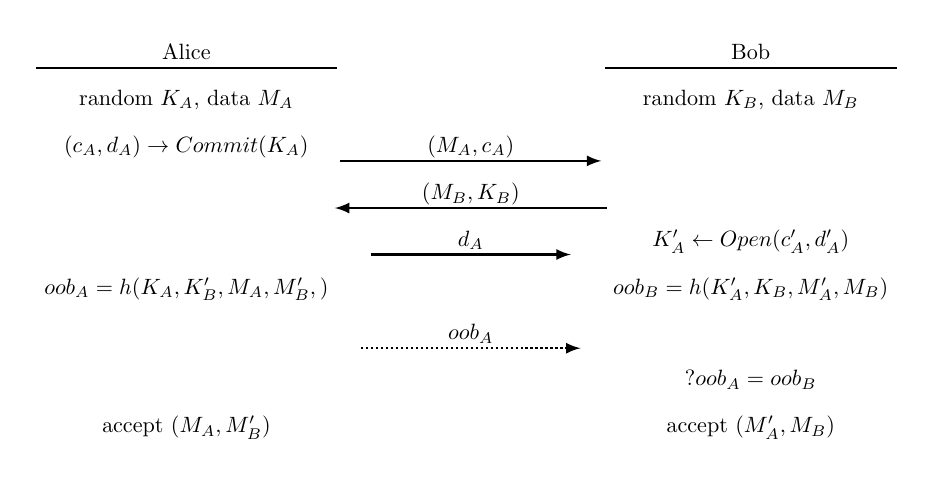
\begin{tikzpicture}[thick,scale=0.8, every node/.style={scale=0.8}]
\matrix (m)[matrix of nodes, column sep=1cm,row sep=6mm, nodes={draw=none, anchor=center,text depth=0pt} ]{
Alice & & Bob\\[-4mm]
random $K_A$, data $M_A$ & & random $K_B$, data $M_B$ \\[-4mm]
$(c_A,d_A)\rightarrow Commit(K_A)$ & $(M_A,c_A)$ & \\[- 4mm]
						 & $(M_B,K_B)$ & \\[- 4mm]
						 & $d_A$ & $K'_A \leftarrow Open(c'_A,d'_A)$ \\[-4mm]
$oob_A = h(K_A,K'_B,M_A,M'_B,)$ & & $oob_B = h(K'_A,K_B,M'_A,M_B)$\\ [-4mm]
							&$oob_A$& \\ [-4mm]
 							& & $?oob_A = oob_B$ \\ [-4mm]
accept $(M_A,M'_B)$ & & accept $(M'_A,M_B)$ \\ [-4mm]
};

\draw[shorten <=-1.5cm,shorten >=-1.5cm] (m-1-1.south east)--(m-1-1.south west);
\draw[shorten <=-1.5cm,shorten >=-1.5cm] (m-1-3.south east)--(m-1-3.south west);
\draw[shorten <=-1cm,shorten >=-1cm,-latex] (m-3-2.south west)--(m-3-2.south east);
\draw[shorten <=-1cm,shorten >=-1cm,-latex] (m-4-2.south east)--(m-4-2.south west);
\draw[shorten <=-1cm,shorten >=-1cm,-latex] (m-5-2.south west)--(m-5-2.south east);
\draw[shorten <=-1cm,shorten >=-1cm,-latex,densely dotted] (m-7-2.south west)--(m-7-2.south east);
\end{tikzpicture}
\end{center}

\subsubsection*{Manually authenticated MA-DH}

When revising MANA IV protocol, Laur and Kyberg~\cite{Laur:2006kl} indicated that the protocol was not computational efficiency. For this reason, they proposed a new modified protocol, namely Manually Authenticated Diffie-Hellman (MA-DH). The protocol runs as follows. 
 
\begin{enumerate}
\item Alice computes $(c,d) \leftarrow Commit(K_A)$ for $K_A = g^a$, and sends $(ID_A, c)$ to Bob.
\item Bob computes $K_B = g^b$ for a random $b$, and sends $ (ID_B,K_B)$ to Alice.
\item Alice sends $d$ to Bob. 
\item Bob computes $K'_A \leftarrow Open(c',d')$ and halts if $K'_A = NULL$. Both parties compute $sid = (ID_A,ID_B)$ and $oob= h(sid,ka,kb)$.
\item Both parties accept $key = (g^a)^b = (g^b)^a$ iff the l-bit test values $oob_a$ and $oob_b$ coincide. 
\end{enumerate}

\begin{center}
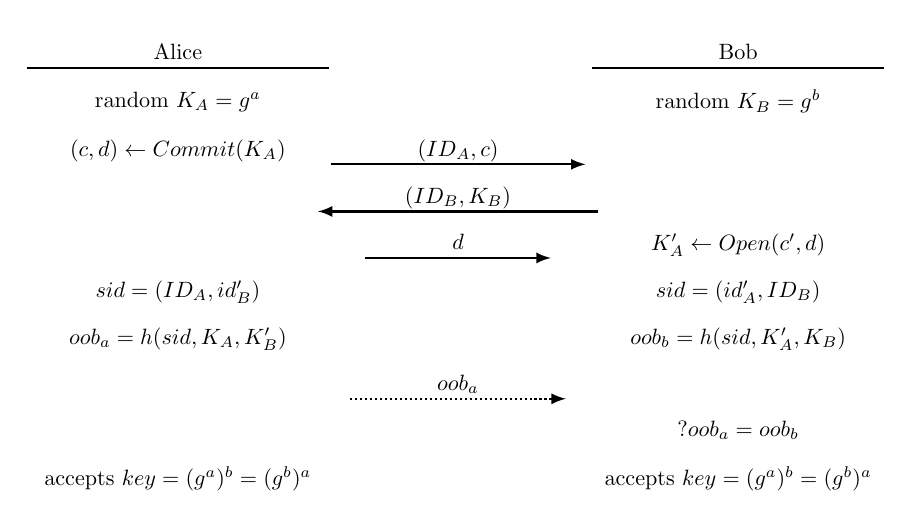
\begin{tikzpicture}[thick,scale=0.8, every node/.style={scale=0.8}]
\matrix (m)[matrix of nodes, column sep=1cm,row sep=6mm, nodes={draw=none, anchor=center,text depth=0pt} ]{
Alice & & Bob\\[-4mm]
random $K_A = g^a$		 & & random $K_B = g^b$ \\[-4mm]
$(c,d) \leftarrow Commit(K_A)$ &$(ID_A,c)$ & \\[- 4mm]
						& $(ID_B,K_B)$ & \\[- 4mm]
						& $d$ & $K'_A \leftarrow Open(c',d)$ \\[-4mm]
$sid=(ID_A,id'_B)$			& & $sid=(id'_A,ID_B)$	\\[-4mm]
$oob_a =h(sid,K_A,K'_B)$ & & $oob_b =h(sid,K'_A,K_B)$\\[-4mm]
					 & $oob_a$& \\ [-4mm]
 					 & & $?oob_a = oob_b$\\ [-4mm]
 accepts $key =(g^a)^b = (g^b)^a$ & & accepts $key =(g^a)^b = (g^b)^a$ \\ [-4mm] 
};

\draw[shorten <=-1.5cm,shorten >=-1.5cm] (m-1-1.south east)--(m-1-1.south west);
\draw[shorten <=-1.5cm,shorten >=-1.5cm] (m-1-3.south east)--(m-1-3.south west);
\draw[shorten <=-1cm,shorten >=-1cm,-latex] (m-3-2.south west)--(m-3-2.south east);
\draw[shorten <=-1cm,shorten >=-1cm,-latex] (m-4-2.south east)--(m-4-2.south west);
\draw[shorten <=-1cm,shorten >=-1cm,-latex] (m-5-2.south west)--(m-5-2.south east);
\draw[shorten <=-1cm,shorten >=-1cm,-latex,densely dotted] (m-8-2.south west)--(m-8-2.south east);
\end{tikzpicture}
\end{center}

\subsubsection*{Analysis of SAS-Based Protocols}

Vaudenay and Pasini used Bellare-Rogaway model to prove their protocols. They also claimed that attack success probability is $2^{-k}$ for k-bit SAS, and $Q_A Q_B 2^{-k}$ where $Q_A$ and $Q_B$ are a number of instance of Alice and Bob in network. For instance, $k$ is 50-bits in multi-party network, and 15-bits in 2-party network.

However, Laur and Nyberg in \cite{Laur:2006kl} did not agree with Vaudenay results because their proofs are not sufficient, and Random Oracle(RO) model and Common Reference String (CRS) model are not suitable for ad hoc networks.

Laur and Nyberg showed in their model that attack success probability against MANA IV and DA-DH is $2^ {-k}$ where $k$ is length of SAS value.

\subsubsection{Cagalj-Capkun-Huxbaux Protocols}

Cagalj, Capkun and Huxbaux \cite{1580514} proposed three various protocols which are based on original DH protocol, and are assisted by human operations. The first protocol is based on visual comparison of short strings (DH-SC), the second one on distance bounding(DH-DB), and the third one on integrity codes(DH-IC). Each of them is presented below. 
 
\subsubsection*{Diffie-Hellman key agreement protocol with String Comparison}

\begin{enumerate}
\item Alice and Bob selects secret exponents $X_A$ and $X_B$, and choose random number $r_a$ and $r_b$ respectively. 
\item Alice and Bob calculate DH public parameters $g^a$ and $g^b$. 
\item Alice computes $m_A \leftarrow 0||ID_A||g^a||r_a$. Bob computes $m_B \leftarrow 1||ID_B||g^b||r_b$ .
\item Alice computes $(c_A,d_A) \leftarrow Commit(m_A)$ and sends $(c_A)$ to Bob.
\item Bob computes $(c_B,d_B) \leftarrow Commit(M_B)$ , and sends $(c_B)$ to Alice.
\item Alice sends $d_A$ to Bob. Bob computes $M'_A \leftarrow Open(c'_A,d'_A)$ and verifies that 0 appears at beginning of $M'_A$. If verification is successful, Bob sends $d_B$ to Alice.
\item Alice computes $M'_B \leftarrow Open(c'_B,d'_B)$ and verifies that 1 appears at beginning of $M'_B$
 \item If the verification of Alice is successful, both parties go to the next stage.
\item Alice computes $i_A \leftarrow r'_b \oplus r_a$, Bob computes $i_B \leftarrow r_b \oplus r'_a$.
\item Bob sides exchange their short values over an out-of-band channel. If the received value equals the computed value, each side informs a successful signal. 
\end{enumerate}

Note that, 0 and 1 are public values used to prevent reflection attack. The identification $ID_A$ and $ID_B$ are human readable, e.g. email addresses or names. The authors used screens or human-voice as an out-of-band channel to securely transmit authenticated values.
 
\begin{center}
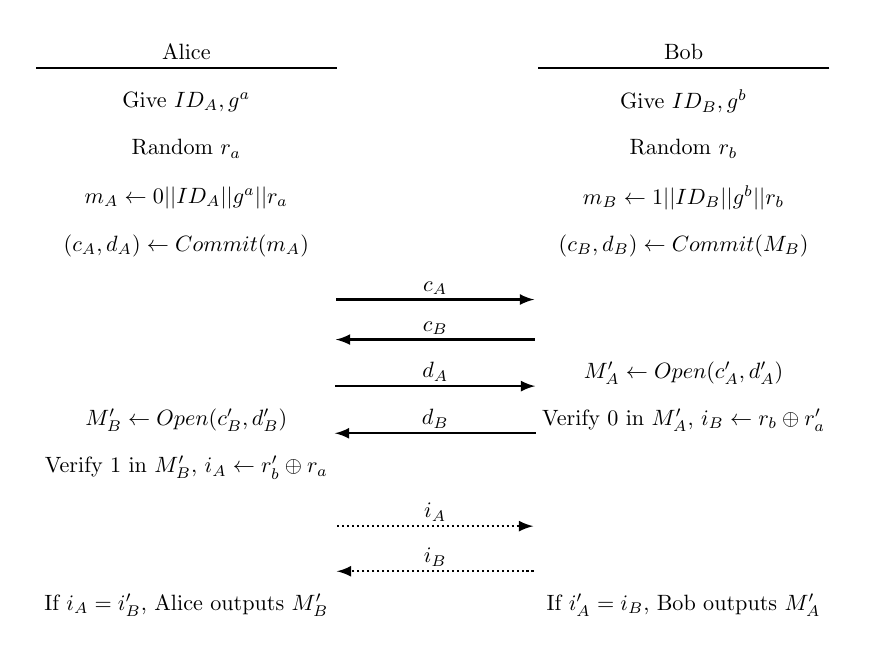
\begin{tikzpicture}[thick,scale=0.8, every node/.style={scale=0.8}]
\matrix (m)[matrix of nodes, column sep=1cm,row sep=6mm, nodes={draw=none, anchor=center,text depth=0pt} ]{
Alice & & Bob\\[-4mm]
Give $ID_A,g^a$		 & & Give $ID_B,g^b$ \\[-4mm]
Random $r_a $		 & & Random $r_b $ \\[-4mm]
$m_A \leftarrow 0||ID_A||g^a||r_a$ & & $m_B \leftarrow 1||ID_B||g^b||r_b$ \\[- 4mm]
$(c_A,d_A) \leftarrow Commit(m_A)$ & & $(c_B,d_B) \leftarrow Commit(M_B)$ \\[- 4mm]
						& $c_A$ & \\[- 4mm]
						& $c_B$ & \\[- 4mm]
						& $d_A$ & $M'_A \leftarrow Open(c'_A,d'_A)$\\[- 4mm]
$M'_B \leftarrow Open(c'_B,d'_B)$ & $d_B$ & Verify 0 in $M'_A$, $i_B \leftarrow r_b \oplus r'_a$\\[- 4mm]
Verify 1 in $M'_B$, $i_A \leftarrow r'_b \oplus r_a$	& & \\[-4mm]
						& $i_A$ & \\[-4mm]
						& $i_B$ & \\[-4mm]
If $i_A = i'_B$, Alice outputs $M'_B$ & & If $i'_A = i_B$, Bob outputs $M'_A$ \\ [-4mm] 
};

\draw[shorten <=-1.5cm,shorten >=-1.5cm] (m-1-1.south east)--(m-1-1.south west);
\draw[shorten <=-1.5cm,shorten >=-1.5cm] (m-1-3.south east)--(m-1-3.south west);

\draw[shorten <=-1cm,shorten >=-1cm,-latex] (m-6-2.south west)--(m-6-2.south east);
\draw[shorten <=-1cm,shorten >=-1cm,-latex] (m-7-2.south east)--(m-7-2.south west);
\draw[shorten <=-1cm,shorten >=-1cm,-latex] (m-8-2.south west)--(m-8-2.south east);
\draw[shorten <=-1cm,shorten >=-1cm,-latex] (m-9-2.south east)--(m-9-2.south west);
\draw[shorten <=-1cm,shorten >=-1cm,-latex,densely dotted] (m-11-2.south west)--(m-11-2.south east);
\draw[shorten <=-1cm,shorten >=-1cm,-latex,densely dotted] (m-12-2.south east)--(m-12-2.south west);
\end{tikzpicture}
\end{center}
\subsubsection*{Diffie-Hellman key agreement protocol with Distance Bounding}

Distance bounding protocol allows both devices to verify the distance between them. Hence, this protocol can act as a secure channel. 

Protocol DH-DB is mainly built on the DH-SC. Upon reception of commitment $d_A,d_B$, both devices execute distance bounding protocol to exchange $r_a,r_b, i_A, i_B$. According to time-flight estimation, each device can extract upper bound distance of the other devices. 

Finally, both devices exchange $y_A$, and $y_B$ to open the commitment $x_A, x_B$ respectively. At the last step, each device check if $i'_A,i'_B$ and $i_A,i_B$ equal or not.  Note that, this last step is done by device itself, whereas in DH-SC the comparison is performed by the users. 

\begin{center}
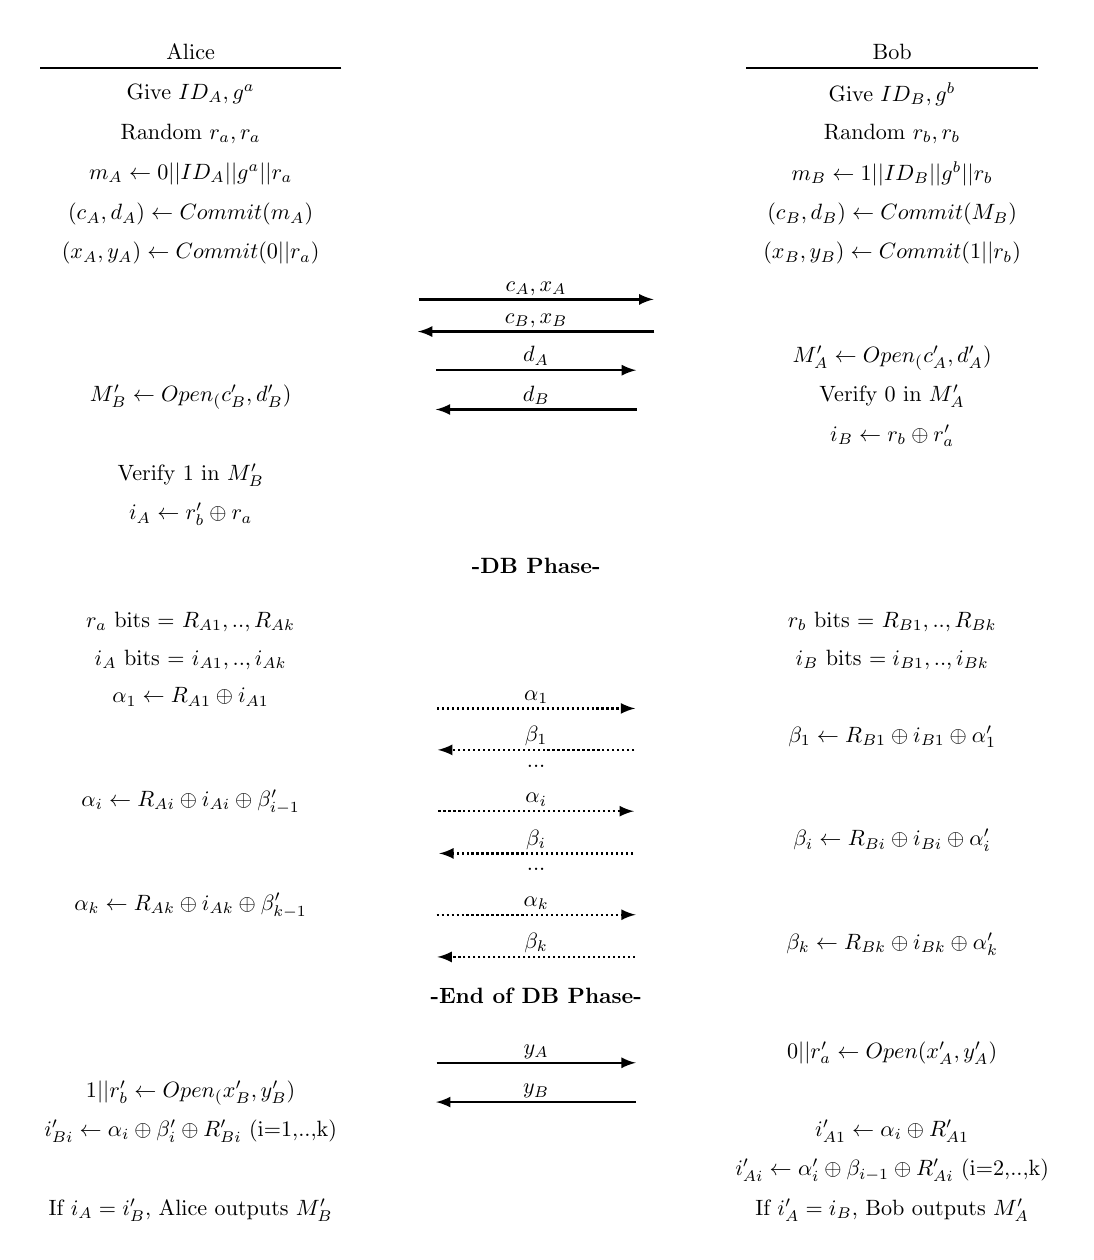
\begin{tikzpicture}[thick,scale=0.8, every node/.style={scale=0.8}]
\matrix (m)[matrix of nodes, column sep=1cm,row sep=5mm, nodes={draw=none, anchor=center,text depth=0pt} ]{

Alice & & Bob\\[-4mm]
Give $ID_A,g^a$		 & & Give $ID_B,g^b$ \\[- 4mm]
Random $r_a,r_a $		 & & Random $r_b,r_b $ \\[- 4mm]
$m_A \leftarrow 0||ID_A||g^a||r_a$ & & $m_B \leftarrow 1||ID_B||g^b||r_b$ \\[- 4mm]
$(c_A,d_A) \leftarrow Commit(m_A)$ & & $(c_B,d_B) \leftarrow Commit(M_B)$ \\[- 4mm]
$(x_A,y_A) \leftarrow Commit(0||r_a)$ & & $(x_B,y_B) \leftarrow Commit(1||r_b)$ \\[- 4mm]
						& $c_A,x_A$ & \\[-4mm]
						& $c_B,x_B$ & \\[-4mm]
						& $d_A$ & $M'_A \leftarrow Open_(c'_A,d'_A)$\\[-4mm]
$M'_B \leftarrow Open_(c'_B,d'_B)$ & $d_B$ & Verify 0 in $M'_A$\\[-4mm]
						& &	$i_B \leftarrow r_b \oplus r'_a$\\[-4mm]
Verify 1 in $M'_B$ 	& & \\[-4mm]
$i_A \leftarrow r'_b \oplus r_a$	& & \\[-2mm]
					& \textbf{-DB Phase-} & \\[-2mm]
$r_a$ bits = $R_{A1},..,R_{Ak}$ & & $r_b$ bits = $R_{B1},..,R_{Bk}$ \\[-4mm]
$i_A$ bits = $i_{A1},..,i_{Ak}$ & & $i_B$ bits $= i_{B1},..,i_{Bk}$	\\[-4mm]
$\alpha_1 \leftarrow R_{A1} \oplus i_{A1}$ & $\alpha_1$ & \\[-4mm]
					& $\beta_1$ & 	$\beta_1 \leftarrow R_{B1} \oplus i_{B1} \oplus \alpha'_1$ \\[-4mm]
					& ... & \\[-4mm]
$\alpha_i \leftarrow R_{Ai} \oplus i_{Ai} \oplus \beta'_{i-1}$ & $\alpha_i$ & \\[-4mm]
					& $\beta_i$ & 	$\beta_i \leftarrow R_{Bi} \oplus i_{Bi} \oplus \alpha'_i$ \\[-4mm]
					& ... & \\[-4mm]
$\alpha_k \leftarrow R_{Ak} \oplus i_{Ak} \oplus \beta'_{k-1}$ & $\alpha_k$ & \\[-4mm]
					& $\beta_k$ & 	$\beta_k \leftarrow R_{Bk} \oplus i_{Bk} \oplus \alpha'_k$ \\[-2mm]
					& \textbf{-End of DB Phase-} & \\[-2mm]
					& $y_A$ & $0||r'_a \leftarrow Open(x'_A,y'_A)$ \\[-4mm]
$1||r'_b \leftarrow Open_(x'_B,y'_B)$ & $y_B$ & \\[-4mm]
$i'_{Bi} \leftarrow \alpha_i \oplus \beta'_i \oplus R'_{Bi}$ (i=1,..,k) & & $i'_{A1} \leftarrow \alpha_i \oplus R'_{A1}$ \\[-4mm] 
& & $i'_{Ai} \leftarrow \alpha'_i \oplus \beta_{i-1} \oplus R'_{Ai}$ (i=2,..,k) \\[-4mm]
If $i_A = i'_B$, Alice outputs $M'_B$ & & If $i'_A = i_B$, Bob outputs $M'_A$ \\ [-4mm] 
};
\draw[shorten <=-1.5cm,shorten >=-1.5cm] (m-1-1.south east)--(m-1-1.south west);
\draw[shorten <=-1.5cm,shorten >=-1.5cm] (m-1-3.south east)--(m-1-3.south west);

\draw[shorten <=-1cm,shorten >=-1cm,-latex] (m-7-2.south west)--(m-7-2.south east);
\draw[shorten <=-1cm,shorten >=-1cm,-latex] (m-8-2.south east)--(m-8-2.south west);
\draw[shorten <=-1cm,shorten >=-1cm,-latex] (m-9-2.south west)--(m-9-2.south east);
\draw[shorten <=-1cm,shorten >=-1cm,-latex] (m-10-2.south east)--(m-10-2.south west);

\draw[shorten <=-1cm,shorten >=-1cm,-latex,densely dotted] (m-17-2.south west)--(m-17-2.south east);
\draw[shorten <=-1cm,shorten >=-1cm,-latex,densely dotted] (m-18-2.south east)--(m-18-2.south west);
\draw[shorten <=-1cm,shorten >=-1cm,-latex,densely dotted] (m-20-2.south west)--(m-20-2.south east);
\draw[shorten <=-1cm,shorten >=-1cm,-latex,densely dotted] (m-21-2.south east)--(m-21-2.south west);
\draw[shorten <=-1cm,shorten >=-1cm,-latex,densely dotted] (m-23-2.south west)--(m-23-2.south east);
\draw[shorten <=-1cm,shorten >=-1cm,-latex,densely dotted] (m-24-2.south east)--(m-24-2.south west);

\draw[shorten <=-1cm,shorten >=-1cm,-latex] (m-26-2.south west)--(m-26-2.south east);
\draw[shorten <=-1cm,shorten >=-1cm,-latex] (m-27-2.south east)--(m-27-2.south west);

\end{tikzpicture}
\end{center}

\subsubsection*{Diffie-Hellman key agreement protocol with Integrity Codes}

Integrity codes (I-codes) are used with communication channel such that that they are not possible to block signal without being detected. An integrity code is a seven-tuple $(\mathcal{S},\mathcal{M},\mathcal{E},\mathcal{P},l,t,e_c)$ where:
\begin{enumerate}
\item $\mathcal{S}$ is possible of source states. 
\item $\mathcal{M}$ is a set of binary of sequence $t$ 1's and $l-t$ 0's. 
\item $\mathcal{E}$ is a set of source encoding rules $e_s: \mathcal{S} \rightarrow \mathcal{M}$, where $e_s \in \mathcal{E}$ is an injective function. 
\item $\mathcal{P}$ is a set consisting of two power levels 0 and $p$ with $p > 0$.
\item $e_c:\mathcal{M} \rightarrow \mathcal{P^l}$ is a channel modulation function satisfying rules: (i) symbol "1" is transmitted using power level $p$, symbol "0" is transmitted using power level 0. 
\end{enumerate} 

Based on a concept of I-codes, its application on DH-SC is straightforward. Bob and Alice complete four steps of DH-SC protocol at beginning. Alice encoded authentication value $i_A$ into $I-code$, then transmits it in an out-of-band channel to Bob. After reception of $I-code$, Bob probably ensures that this $I-code$ is sent from Alice, and verifies if authenticated value $i'_A$ is equal to $i_B$ or not. 
 
\begin{center}
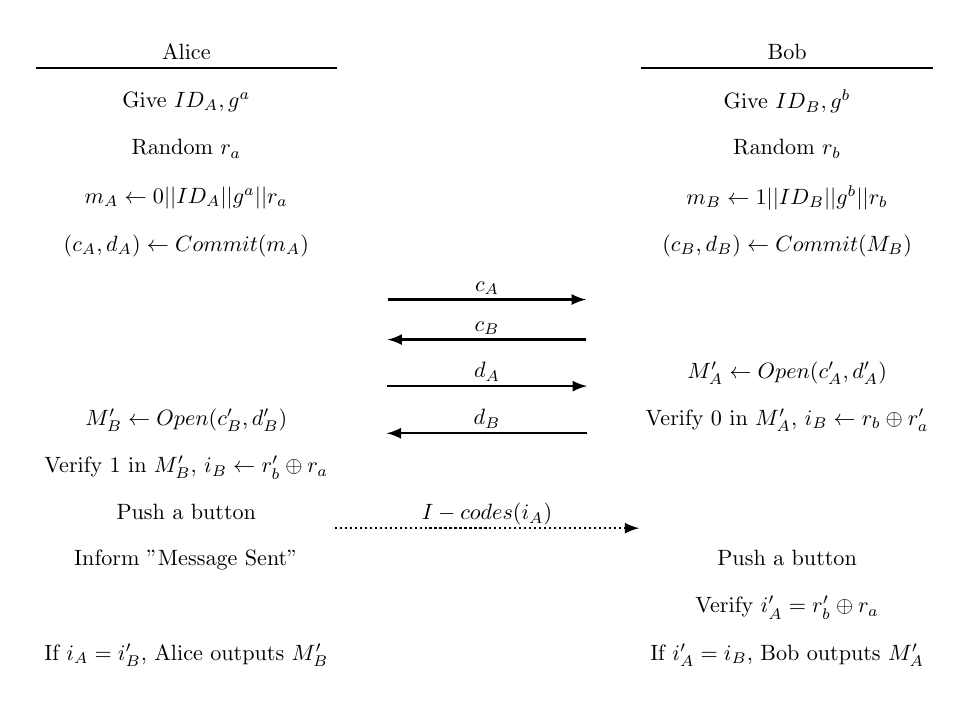
\begin{tikzpicture}[thick,scale=0.8, every node/.style={scale=0.8}]
\matrix (m)[matrix of nodes, column sep=1cm,row sep=6mm, nodes={draw=none, anchor=center,text depth=0pt} ]{
Alice & & Bob\\[-4mm]
Give $ID_A,g^a$		 & & Give $ID_B,g^b$ \\[-4mm]
Random $r_a $		 & & Random $r_b $ \\[-4mm]
$m_A \leftarrow 0||ID_A||g^a||r_a$ & & $m_B \leftarrow 1||ID_B||g^b||r_b$ \\[- 4mm]
$(c_A,d_A) \leftarrow Commit(m_A)$ & & $(c_B,d_B) \leftarrow Commit(M_B)$ \\[- 4mm]
						& $c_A$ & \\[- 4mm]
						& $c_B$ & \\[- 4mm]
						& $d_A$ & $M'_A \leftarrow Open(c'_A,d'_A)$\\[- 4mm]
$M'_B \leftarrow Open(c'_B,d'_B)$ & $d_B$ & Verify 0 in $M'_A$, $i_B \leftarrow r_b \oplus r'_a$\\[- 4mm]
Verify 1 in $M'_B$, $i_B \leftarrow r'_b \oplus r_a$	& & \\[-4mm]
Push a button			& $I-codes(i_A)$ & \\[-4mm]
Inform "Message Sent" & & Push a button \\[-4mm]
					& & Verify $i'_A = r'_b \oplus r_a$ \\[-4mm]
If $i_A = i'_B$, Alice outputs $M'_B$ & & If $i'_A = i_B$, Bob outputs $M'_A$ \\ [-4mm] 
};

\draw[shorten <=-1.5cm,shorten >=-1.5cm] (m-1-1.south east)--(m-1-1.south west);
\draw[shorten <=-1.5cm,shorten >=-1.5cm] (m-1-3.south east)--(m-1-3.south west);

\draw[shorten <=-1cm,shorten >=-1cm,-latex] (m-6-2.south west)--(m-6-2.south east);
\draw[shorten <=-1cm,shorten >=-1cm,-latex] (m-7-2.south east)--(m-7-2.south west);
\draw[shorten <=-1cm,shorten >=-1cm,-latex] (m-8-2.south west)--(m-8-2.south east);
\draw[shorten <=-1cm,shorten >=-1cm,-latex] (m-9-2.south east)--(m-9-2.south west);
\draw[shorten <=-1cm,shorten >=-1cm,-latex,densely dotted] (m-11-2.south west)--(m-11-2.south east);
\end{tikzpicture}
\end{center}

\subsubsection{Short Random String-Based Key Agreement Protocol}

Authors in~\cite{5678019} claimed that SAS-based AKA methods strongly required assistance from users. Therefore, they proposed a scheme, namely Short Random String (SRS)-based key agreement protocol, automatically pairing two devices using an audio channel. The proposed scheme was claimed more advantage than SAS-based scheme in term of bandwidth utilisation. 

The 3-move protocol between $Alice$ and $Bob$ is as follow.
\begin{enumerate}
\item A device $A$ sends A's public key $PK_A$ to device $B$.
\item A device $B$ generates two random strings, $r$ and $SRS$. Then $B$ calculates a hashed value using $PK_A$, $PK_B$, $SRS$ and $r$ and sends this value to $A$.
\item $B$ sends $SRS$ to $A$ over an out-of-band channel. 
\item $B$ sends $r$ to $A$.
\item $A$ verifies the hashed value received in step 2 using $PK_A$, $PK_B$, $SRS$ and $R$. If it is successful, $A$ generates agreed key using authenticated B's public key. 
\end{enumerate}

In the protocol, the verification process is only decided by $A$, then attackers easily impersonate A's public key. However, this attack can be prevented by human monitoring or confirming from $A$to $B$. 

\begin{center}
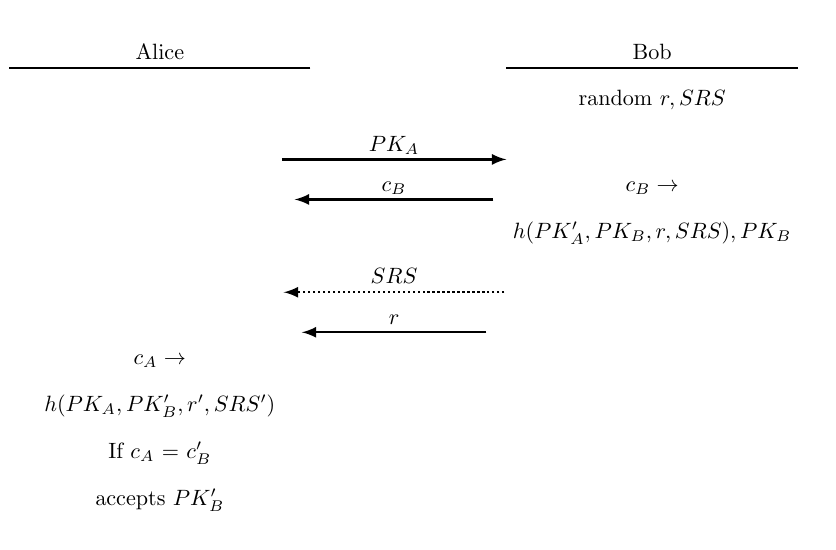
\begin{tikzpicture}[thick,scale=0.8, every node/.style={scale=0.8}]
\matrix (m)[matrix of nodes, column sep=1cm,row sep=6mm, nodes={draw=none, anchor=center,text depth=0pt} ]{
Alice & & Bob\\[-4mm]
						 & & random $r, SRS$ \\[-4mm]
						 & $PK_A$ & \\[- 4mm]
						& $c_B$ & $ c_B\rightarrow$ \\ [- 4mm]
						& & $h(PK'_A,PK_B,r,SRS),PK_B$\\[- 4mm]
									& $SRS$ & \\[-4mm]
								 & $r$ & \\[-4mm]
$c_A \rightarrow $ & & \\[-4mm]
$h(PK_A,PK'_B,r',SRS')$ & & \\[-4mm]
If $c_A$ = $c'_B$ & & \\ [-4mm]
 accepts $PK'_B$		 	 & & \\ [-4mm] 
};

\draw[shorten <=-1.5cm,shorten >=-1.5cm] (m-1-1.south east)--(m-1-1.south west);
\draw[shorten <=-1.5cm,shorten >=-1.5cm] (m-1-3.south east)--(m-1-3.south west);
\draw[shorten <=-1cm,shorten >=-1cm,-latex] (m-3-2.south west)--(m-3-2.south east);
\draw[shorten <=-1cm,shorten >=-1cm,-latex] (m-4-2.south east)--(m-4-2.south west);
\draw[shorten <=-1cm,shorten >=-1cm,-latex,densely dotted] (m-6-2.south east)--(m-6-2.south west);
\draw[shorten <=-1cm,shorten >=-1cm,-latex] (m-7-2.south east)--(m-7-2.south west);
\end{tikzpicture}
\end{center} 

Strength of the protocol completely lies on length of SRS string. If the length of SRS message is $p$, then success probability of attack is less than or equal $2^{-p}$. 

Summing up this part is presented at the table \ref{paircom}.

\begin{table}[ht] 
\centering
\caption{\textsc{Paring Method Comparision}}
\label{paircom}
{\scriptsize
\begin{tabular}{ | p{2cm} | p{1.4cm} | p{1.4cm} | p{2cm} | p{2.2cm} | p{2cm} | p{2cm}| }
\hline
\textbf{Approach} &\multicolumn{2}{c}{ \textbf{Number of Message}} & \textbf{Computation} & \textbf{Communication} & \textbf{Required Cryptographic} & \textbf{Comment}\\ 
 & \textbf{Wireless Channel} & \textbf{OOB Channel} & \textbf{Cost per Sid} & \textbf{Cost over OOB} & \textbf{Primitives} & \\ \hline \hline

Maher Manual Authentication & 2 & 2 & 1 CF & 2* 80 bits & CF & Long OOB message \\ \hline

Talking to Strangers & 2 &	 2	& 1 HASH &	 2 ID + 2 HASH	& HF	& Not specific HASH output length, long OOB message \\ \hline 

VIC & 3	& 1	& 1 HASH 	 & 20 bits HASH	& HF & Long OOB message \\ \hline 

MANA I	& 0	& 1	& 1 CF & 20 bits K + 20bits CV	& CF & \\ \hline 

MANA II	& 1	& 1 & 1 CF & 20 bits K + 20bits CV	& CF & \\ \hline 

MANA III	& 4	& 1 & 2 * HASH	& 16-20bits K & MAC & \\ \hline 

Wong-Stajano MANA III & 6 & 2	& 1 MAC	& 2 *(20 bits N) & HF & \\ \hline 

Wong-Stajano Bidirectional Out-of-band Channel & 4	 & 2	& 1 MAC & 2 *(20 bits N) 	 & HF	 & \\ \hline 

Wong-Stajano Unidirectional Out-of-band Channel & 3 &	 1	& 1 MAC	 & 20 bits N &	 HF & \\ \hline 

Improved Wong-Stajano & 4	& 1	& 1 HASH + 1 XOR	 & 1* (20 bits N) &	 HF + XOR & \\ \hline 

Hoepman AKA & 4	& 2 &	 1 L\_HASH + 1 S\_HASH & 	2* (n bits S\_HASH) &	 Short(S\_) and Long(L\_) HF & n is unclear, fresh random DH public keys \\ \hline 

Improved	Ephemeral Pairing & 3 &	 1 &	 1 L\_HASH + 1 S\_HASH &	80 bits S\_HASH & Short(S\_) and Long(L\_) HF & fresh random DH public keys \\ \hline 
 
4-move SAS Vaudenay & 4	& 2 & 1 CS + 1 XOR & 15bits SAS	& CS + XOR & \\ \hline 

3-move SAS Vaudenay & 3	& 1 & 1 CS + 1 XOR & 15bits SAS	& CS + XOR & \\ \hline 
 																				
SAS Cros AKA Pasini-Vaudenay &	3 &	2 &	1 CS + 1 XOR + 1 HASH & 2 * (15-20bits SAS) & CS + XOR + HF & \\ \hline 

MANA IV & 3 & 1 & 1 CS + 1 HASH & 14bits SAS & CS + HF & \\ \hline 

MA-DH & 3 &	1 &	1 CS + 1 HASH & 14bits SAS & CS + HF & \\ \hline 

 SRS-based AK & 3 & 1 &	1 CS &	 15 bits SRS &	 CS & \\ \hline 

DH-SC & 4 &	2 &	2 CS + 1 XOR & 15bits SAS & CS +XOR & \\ \hline 

DH-DB & 6 &	2 &	1 CS + 1 XOR & 15bits SAS & CS +XOR & \\ \hline \hline 

\textbf{ID} &\multicolumn{2}{c}{Identification} & & & & \\
\textbf{CS} &\multicolumn{2}{c}{Commitment Scheme} & & & & \\
\textbf{XOR} &\multicolumn{2}{c}{XOR operation} & & & & \\
\textbf{CV} &\multicolumn{2}{c}{Check Value} & & & & \\
\textbf{CF} &\multicolumn{2}{c}{Check Function} & & & & \\
\textbf{HF} &\multicolumn{2}{c}{Hash Function} & & & & \\
\textbf{N} &\multicolumn{2}{c}{Nonce} & & & & \\
\textbf{S\_HASH} &\multicolumn{2}{c}{Short Hash} & & & & \\
\textbf{L\_HASH} &\multicolumn{2}{c}{Long Hash} & & & & \\ \hline
\end{tabular}
}
\end{table}

\section{2-Move Secure Device Pairing Protocol}\label{chap42move}

In this section, we propose a novel pairing protocol. This proposal is relatively efficient in sense that it only requires 2 messages on a wireless channel plus one message on a unidirectional public OOB channel. In spite of this, we will see in section~\ref{proof-computational-model} that it still preserves an attack success probability of $2^{-k}$, where $k$ is length of random numbers. The picture~\ref{improved-wong-stajano-protocol} describes how the protocol works. 

The protocol is depicted in Figure ~\ref{improved-wong-stajano-protocol}. It runs between the initiator Alice (A) and the responder Bob (B), who intend to securely exchange their public keys denoted as $g^a$ and $g^b$ respectively. The protocol is presented as below.

\begin{enumerate}
\item Alice picks a random value $r_a$. Bob picks a random value $r_b$
\item Alice sends $(g^a,h(g^a,r_a))$ to Bob.
\item Bob sends $(g^b,r_b)$ to Alice.
\item Alice sends $(r_a \oplus h_{r_b}(g^a,g^b) )$ to Bob over a public channel. 
\item Bob verifies received value and announces the result to Alice. 
\item Alice confirms by pushing an Accept button. 
\end{enumerate}

\begin{figure}[b]
\begin{center}
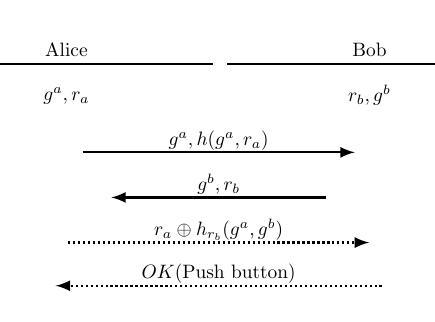
\begin{tikzpicture}[thick,scale=0.7, every node/.style={scale=0.7}]
\matrix (m)[matrix of nodes, column sep=0.5cm,row sep=6mm, nodes={draw=none, anchor=center,text depth=0pt} ]{
Alice & & Bob\\[-4mm]
$g^a,r_a$ & & $r_b,g^b$ \\[-4mm]
					 &$g^a,h(g^a,r_a)$ & \\[- 4mm]
						& $g^b,r_b$ & \\[- 4mm]
						& $r_a \oplus h_{r_b}(g^a,g^b)$ & \\[- 4mm]
& $OK$(Push button) & \\[-4mm]
};

\draw[shorten <=-1.5cm,shorten >=-1.5cm] (m-1-1.south east)--(m-1-1.south west);
\draw[shorten <=-1.5cm,shorten >=-1.5cm] (m-1-3.south east)--(m-1-3.south west);

\draw[shorten <=-1cm,shorten >=-1cm,-latex] (m-3-2.south west)--(m-3-2.south east);
\draw[shorten <=-1cm,shorten >=-1cm,-latex] (m-4-2.south east)--(m-4-2.south west);
\draw[shorten <=-1cm,shorten >=-1cm,-latex,densely dotted] (m-5-2.south west)--(m-5-2.south east);
\draw[shorten <=-1cm,shorten >=-1cm,-latex,densely dotted] (m-6-2.south east)--(m-6-2.south west);

\end{tikzpicture}
\end{center}
\caption{New 2-move Authenticated Key Agreement Protocol} 
\label{improved-wong-stajano-protocol}
\end{figure}

Random values $r_a, r_b$ and use of hash function in the protocol work as an instance of a commitment scheme whose design has strong results on minimising attack probability as we will see in section~\ref{proof-computational-model}. 

This protocol achieves strong security even with a low-bandwidth OOB channel. Alice and Bob are assumed to be honest or uncompromised. After receiving the third message Bob can perform verification and then securely notify Alice of an outcome with the human user's help. 

Table~\ref{devcom} summarises a comparison of our protocol with main existing protocols exploiting a public out-of-band channel. We took into account a number of messages on wireless channel, a number of messages on OOB channel, computation cost, and existence of a formal proof of security (either in the Dolev-Yao model or computational model). In the table, $H$ (resp. $MAC$, $XOR$, $C$) denotes an application of a hash function (resp. a message authentication code, an exclusive-or, a commitment scheme).

In term of computation complexity, our protocol can catch up with other competitors since one exclusive-or operation on a short string does not significantly impact the total cost. Concerning communication cost, our protocol uses the least number of messages. Furthermore, a security 
analysis has been performed both in Dolev-Yao and computational models.

\begin{table}[ht] 
\centering
\caption{\textsc{Device Pairing Protocol Comparison}}
\label{devcom}
{\scriptsize
\begin{tabular}{ p{5cm} l l l l l p{1cm} l p{1cm} l }
\hline
Protocol & Wireless & OOB & Computation Cost & Formal Proof \\
  & Message & Message & & \\
\hline\hline
Bidirectional Wong-Stajano ~\cite{10.1109/MPRV.2007.76} & 4 & 2 & 2*MAC & FAIL \\ \hline
Unidirectional Wong-Stajano ~\cite{10.1109/MPRV.2007.76} & 3 & 2 & 1*MAC & FAIL \\ \hline
Improved Wong-Stajano ~\cite{Nguyen09authenticationprotocols} & 4 & 1 & 2*H + 1*XOR & $\O$ \\ \hline
DH-SC ~\cite{1580514} & 4 & 1 & 2*C + 1*XOR & $\surd$ \\ \hline
4-Move SAS ~\cite{Vaudenay:2005qa} & 4 & 1 & 2*C + 1*XOR & $\surd$ \\ \hline
3-Move SAS ~\cite{Vaudenay:2005qa} & 3 & 1 & 1*C +1H + 1*XOR & $\surd$ \\ \hline
MANA IV ~\cite{Laur:2006kl} & 3 & 1 & 1*C +1*H & $\surd$ \\ \hline
MA-DH ~\cite{Laur:2006kl} & 3 & 1 & 1*C +1*H & $\surd$ \\ \hline
SRS~\cite{5678019} &3 & 1 & 1*H &FAIL \\ \hline 
Our Proposal & 2 & 1 & 1*H +1*MAC + 1*XOR & $\surd$ \\ \hline
\end{tabular}
}
\end{table}

\subsection{Analysis In Computational Model}\label{proof-computational-model}

We give a sketch of proof of our protocol in a computational model. Our goal is to evaluate the successful attacking probability against the protocol. Similarly to~\cite{1580514} we conduct an analysis based on the model presented in~\cite{Bellare:1994aa}. 

We refer to the security definition in~\cite{1580514} which is presented as follows. 

\begin{Definition}
We say that a protocol is a secure protocol enabling authentication of DH public parameter between $A$ and $B$ if attacker cannot succeed in deceiving $A$ and $B$ into accepting DH public parameters different then $g^{xa}$ and $g^{xb}$, except with a satisfactorily small probability $\mathcal{O}(2^{-k})$.
\end{Definition}

\begin{Lemma}\label{lemme5.1}

For any interaction between strand $st$ and $st'$, and attacker $X$, attack success probability of $X$ is lower or equal to $n.\gamma.2^{-k}$, 
where $n$ is the number of participants on the network, $\gamma$ is the maximum number of sessions for each participant, $k$ is the length of short authenticated string. 
\end{Lemma}

\begin{proof}
For a normal run, the responder uses value of $r_a$ extracted from messages received on OOB channel to open the commitment $h(g^a, r_a)$. If the responder opens successfully, an Accept statue is notified. So, to win the game, attacker $X$ has to deliver $h(m)$ in the first message such that $h(m) = h(g^{xa}, (r_a \oplus h_{r_{xb}}(g^a,g^{xb})) \oplus (h_{r_b}(g^{xa},g^b)))$ (1) for some $m$. Due to our assumption on MAC function equation (1) can be rewritten in $h(m) = h(g^{xa}, (r_a \oplus r_{xb} \oplus r_b \oplus h(g^a,g^{xb}) \oplus h(g^{xa},g^b)))$ (2). 

In the simplest case where attacker $X$ is able to find a pair $(g^{xa},g^{xb})$ such that $h(g^{xa},g^b) = h(g^a,g^{xb})$, we can deduce from (2) to $r_{xa} = r_a \oplus r_{xb} \oplus r_b$ or $r_{xa} \oplus r_b = r_a \oplus r_{xb}$ (3).

Observe that $X$ has to submit $r_{xb}$ before actually knowing $r_a$. Similarly, $X$ has to submit $r_{xa}$ before actually seeing $r_b$. Thus irrespectively, the attacking strategy taken by $X$, $r_a$ and $r_b$ will be revealed after $r_{xa}$ and $r_{xb}$ have been generated and submitted. If it happens that both $r_a$ and $r_b$ are revealed in the same time, then we can pick an arbitrary one. 

Assume that $r_a$ is revealed after $r_b$, we have:
\begin{description}
 \item [(i)] $r_a$ and $r_b$ are independently and uniformly distributed random variables, 
 \item [(ii)] $r_{xa}$ and $r_{xb}$ must be generated and submitted before either $r_a$ is revealed, 
 \item [(iii)] each principal can open at most $\gamma$ sessions. 
\end{description}
The same holds for a case where $r_b$ is revealed after $r_a$. Therefore, $Pr[r_{xa} \oplus r_b = r_a \oplus r_{xb}] \leq n.\gamma.2^{-k}$.

In a normal case where $X$ cannot find collision, let $t= h(g^a,g^{xb}) \oplus h(g^{xa},g^b)$ since $g^a$ and $g^b$ are not changed over sessions. We have (i)$r_{xa} \oplus r_b = r_a \oplus r_{xb} \oplus t $, (ii) $t$ could be constant, hence, $Pr[r_{xa} \oplus r_b = r_a \oplus r_{xb} \oplus t ] \leq n.\gamma.2^{-k}$. 
\end{proof}

\subsection{An Implemetation on An Embedded System} 

We produce a prototype of our device pairing protocol using two Arduino boards. Because of lacking WIFI shields, two Ethernet shields are used instead to provide a network connect between two boards. The testing system includes:
\begin{itemize}
\item An Arduino Uno equips with an Ethernet shield, and a LED light.
\item An Arduino Mega equips with an Ethernet shield, and a light sensor.
\item Two boards connect via an Ethernet cable. 
\end{itemize}

The testbed is presented at the figure~\ref{imp}. A visual light communication served as an out-of-band communication channel is intuitively established via a LED and a light sensor. Data transmitting in this channel are encoded by a sequence of blinking light. In particular, while the LED hitting the highest brightness represents for a bit "1", the LED dims to represent for a bit "0". Furthermore, distance between the LED and the light sensor is short enough so that the sensor can correctly recognise bits from the LED. The accuracy of OOB transmission strongly depends on this distance and noise of environment apparently. 

All tests have been done in normal lab environment. We ran 10 times, and in each time 32-bits OOB message was transmitted between two boards. Under 3 centimetres, we get 100\% successful rate. The rate reduces to 75\% in 5 centimetres, and dramatically drops at further distance. However, in low noise environment, the results are remarkably improved. The result of executing time of some functions is presented in the table~\ref{evaluation}. With these results, we believe that our solution is practical.

\begin{figure}
  \centering
  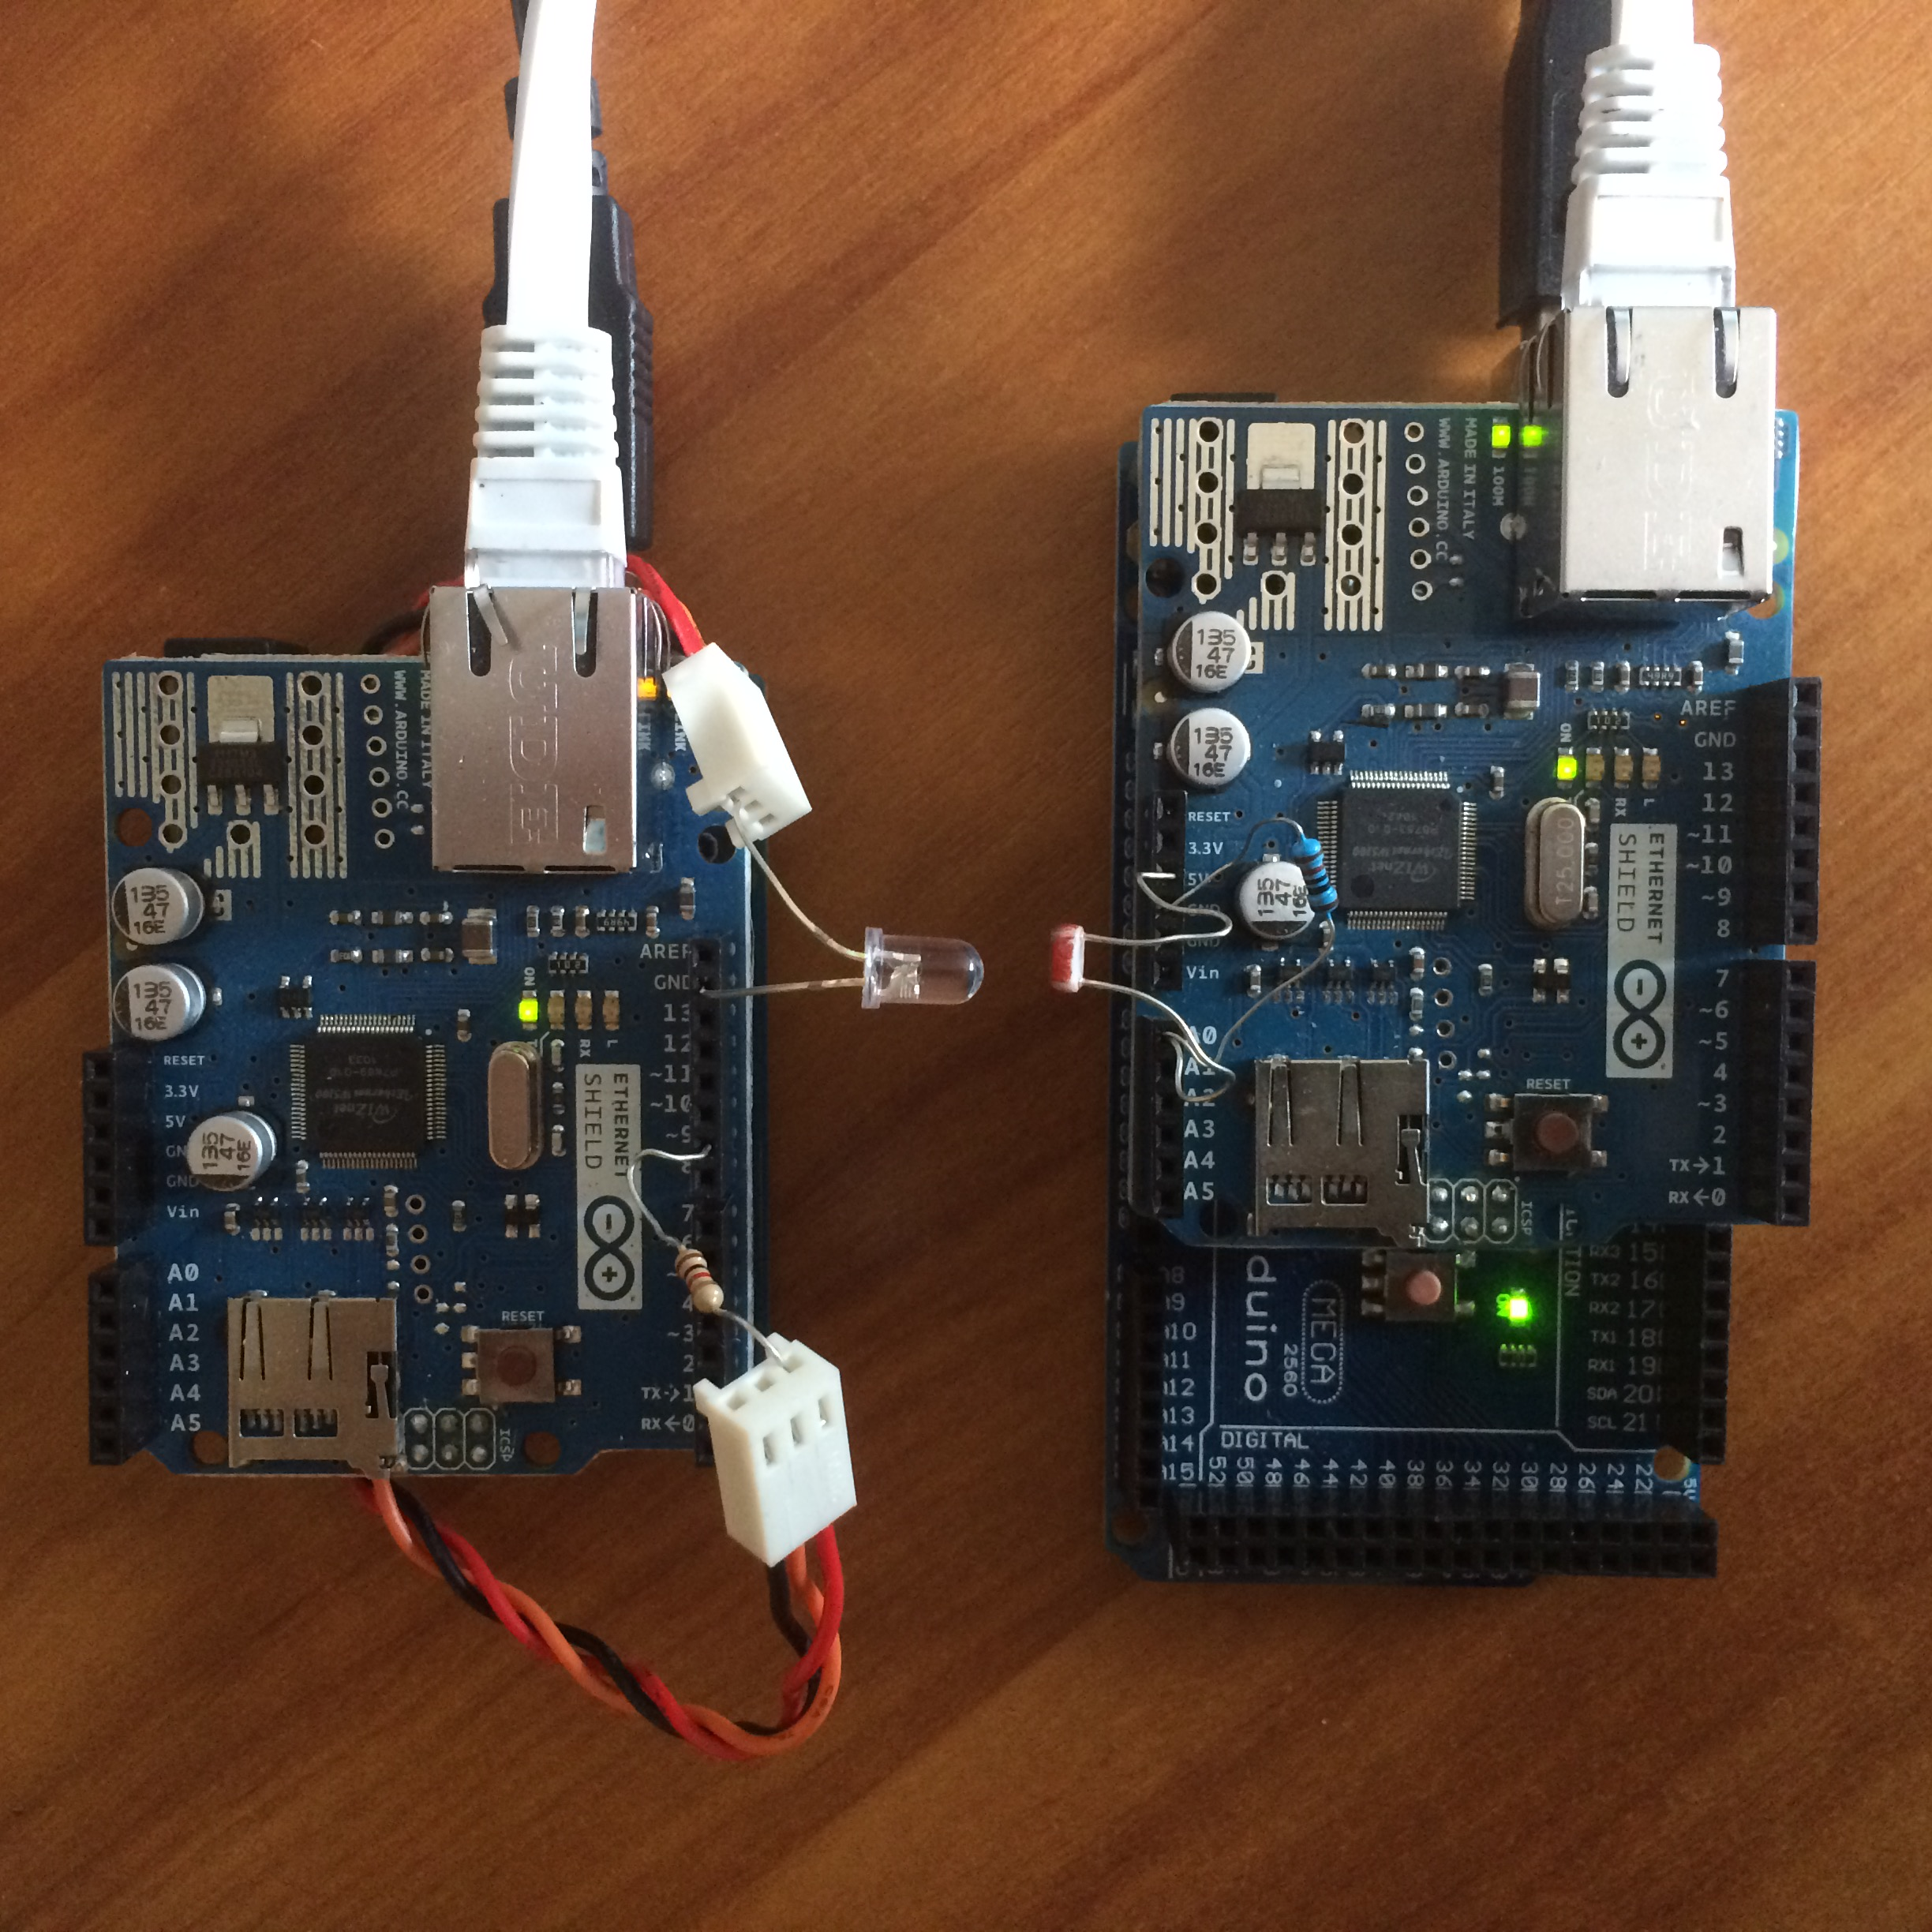
\includegraphics[width=0.5\textwidth]{imp}
  \caption{Prototypes}
  \label{imp}
\end{figure}

\begin{table}[t]
\centering
\caption{\textsc{Performance Evaluation of Device Pairing Protocol}}
\label{evaluation}
{\small
\begin{tabular}{| p{5cm} | p{3cm} |}
 \hline
\textbf{Function} & \textbf{Time(ms)} \\ \hline \hline
Generating Keys & 3898 \\ \hline
Commitment Calculation & 15 \\ \hline
Commitment Validation & 15 \\ \hline
Transferring OOB message & 3201 \\ \hline
Complete Protocol & 21760 \\ \hline
\end{tabular}
}
\end{table}

\section{Flaws Found in Some Pairing Protocols}

In this section, we are going present flaws that we have found in some pairing protocols. These flaws have not revealed in any publication before. 

We will explain clearly how come we can discover these attack in the next chapter. Briefly speaking, we constructed a formal model to analyse our protocol, and adapted it to do other existing device pairing ones introduced in this chapter. As a result of that, some flaws have been discovered. 

To begin with, we would like to take some assumptions on channels, attacker capabilities, and user actions as below. 
\begin{itemize}
\item Two participants don't play the protocol concurrently.
\item The protocol replays when it accidentally gets an error. 
\item Attacker knows OOB message content before the message is delivered.
\item Attacker can delay user's actions. 
\end{itemize}

Furthermore, protocols are considered in theoretical perspective where OOB channels are classified in our category. In particular, these following protocols are assumed to use long-range public out-of-band channels which only provide channel origin authentication.  

\subsection{Attack on Wong-Stajano Protocol using Bidirectional Channel}

The Wong-Stajano protocol using bidirectional channel was presented at~\ref{WS} in this chapter. The protocol aims to provide a key agreement between two participants. However, we found a counterexample in which the protocol goal does not hold for the initiator. The counterexample is illustrated in the figure~\ref{WSbiattack}, and is precisely detailed in table~\ref{WSbiattacktable}. 

\begin{table}[t]
\centering
\caption{\textsc{Attack Scenario Against Initiator's Guarantee in Wong-Stajano Protocol with Bidirectional Channel}}
\label{WSbiattacktable}
{\small
\begin{tabular}{| l | p{11cm} |}
 \hline
 Step 1.1 & Attacker suspends the $r_b$ sent by Bob on OOB channel\\ \hline
 Step 1.2 & Attacker drops the $KB$ sent by Bob. \\ \hline
 Step 1.3 & Attacker starts a new session with Alice\\ \hline \hline
 Step 2.1 & Alice sends $(A, g^{a}, MAC_{KA2}(A,g^{a},R_{A2}))$ to the Attacker on wireless channel\\ \hline
 Step 2.2 & Attacker sends $(B, g^{x}, MAC_{KX}(B,g^{x},R_{B}))$ on wireless channel\\ \hline
 Step 2.3 & Attacker drops $R_{A2}$ sent by Alice on OOB channel\\ \hline
 Step 2.4 & Attacker releases $r_b$ at Step 1.1 on OOB channel \\ \hline
 Step 2.5 & Attacker sends $KX$ to Alice on wireless channel\\ \hline
 Step 2.6 & At the end of the execution, Alice believes she shares a fresh session key with Bob, known actually by the Attacker\\ \hline
\end{tabular}
}
\end{table}

\begin{figure}
  \centering
  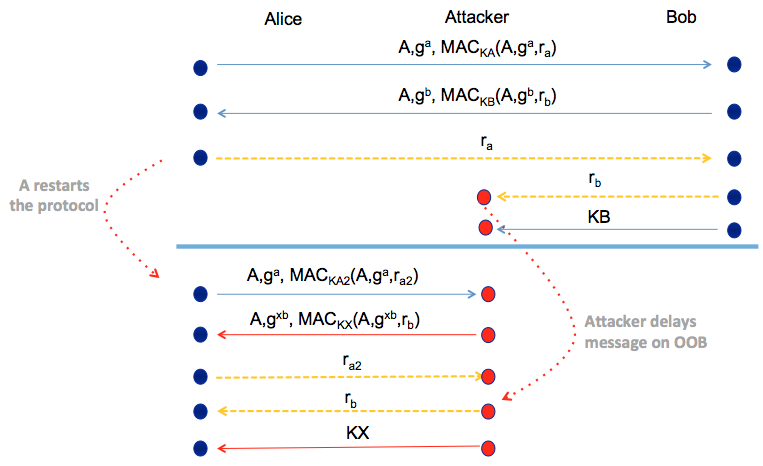
\includegraphics[width=0.9\textwidth]{WSbi}
  \caption{Attack on Wong-Stajano Protocol using Bidirectional Channel with Unidirectional Channel}
  \label{WSbiattack}
\end{figure}

Additionally, we found the protocol is being used in the Pico system of the authors~\cite{Stajano:2014aa}. 
 
\subsection{Attack on Wong-Stajano Protocol using Unidirectional Channel}

The counterexample of Wong-Stajano protocol using unidirectional channel is illustrated in the figure~\ref{WSuniattack}, and is precisely detailed in table~\ref{WSuniattack}. 

\begin{table}[t]
\centering
\caption{\textsc{Attack Scenario Against Initiator's Guarantee in Wong-Stajano Protocol with Unidirectional Channel}}
\label{WSuniattack}
{\small
\begin{tabular}{| l | p{11cm} |}
 \hline
 Step 1.1 & Attacker intercepts $g^{a}$ sent by Alice on wireless channel\\ \hline
 Step 1.2 & Attacker replies with $(B, g^{x}, h_{k_X}(B,g^{x},g^a,r_x))$ to Alice on wireless channel\\ \hline
 Step 1.3 & Attacker suspends $r_b$ sent by Bob on OOB channel, and starts a new session with Alice\\ \hline \hline
 Step 2.1 & Alice sends $g^{a'}$ on wireless channel\\ \hline
 Step 2.2 & Attacker responds $(B, g^{x}, h_{k_X}(B,g^{a'},g^{x'},r_b))$ on wireless channel\\ \hline
 Step 2.3 & Attacker drops $ACK$ sent by Alice on OOB channel\\ \hline
 Step 2.4 & Attacker release $r_b$ sent by Bob on OOB channel at Step 1.3\\ \hline
 Step 2.5 & Attacker sends $k_X$ to Alice on Wireless channel\\ \hline
 Step 2.6 & At the end of the execution, Alice believes she shares a fresh session key with Bob, known actually by the Attacker\\ \hline
\end{tabular}
}
\end{table}

\begin{figure}
  \centering
  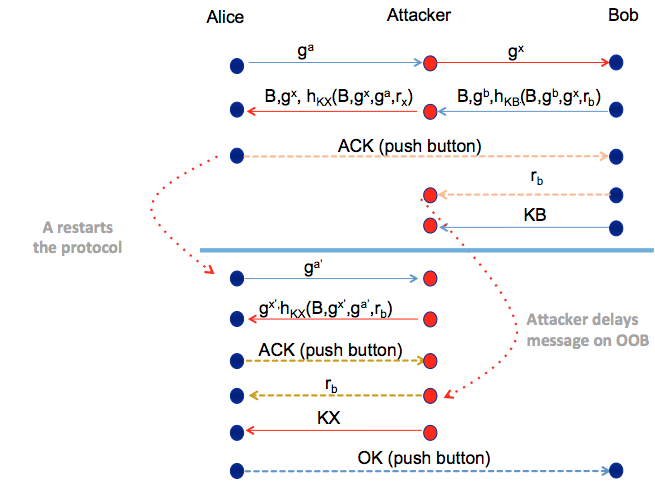
\includegraphics[width=0.8\textwidth]{WSuni}
  \caption{Attack on Wong-Stajano Protocol using Unidirectional Channel}
  \label{WSuniattack}
\end{figure}

\subsection{Attack on SRS-AKA Protocol}

Attack against SRS-AKA is closely identified with one in Wong-Stajano protocol using unidirectional channels. The attack scenario is illustrated in figure~\ref{SRSattack} and detailed at table~\ref{SRSattacktable}.

\begin{table}[t]
\centering
\caption{\textsc{Attack Scenario Against Initiator's Guarantee in SRS-AKA Protocol}}
\label{SRSattacktable}
{\small
\begin{tabular}{| l | p{11cm} |}
 \hline
 Step 1.1 & Attacker intercepts $PK_A$ sent by Alice on wireless channel\\ \hline
 Step 1.2 & Attacker replies with $h(PK_A,PK_X,r_x,SRS_X), PK_X$ to Alice on wireless channel\\ \hline
 Step 1.3 & Attacker suspends $SRS$ sent by Bob on OOB channel, and starts a new session with Alice\\ \hline \hline
 Step 2.1 & Alice sends $PK_A$ on wireless channel\\ \hline
 Step 2.2 & Attacker responds $h(PK_A,PK_X,r_x,SRS), PK_X$  on wireless channel\\ \hline
 Step 2.4 & Attacker release $SRS$ sent by Bob on OOB channel at Step 1.3\\ \hline
 Step 2.5 & Attacker sends $r_x$ to Alice on Wireless channel\\ \hline
 Step 2.6 & At the end of the execution, Alice believes she shares a fresh session key with Bob, known actually by the Attacker\\ \hline
\end{tabular}
}
\end{table}

\begin{figure}
  \centering
  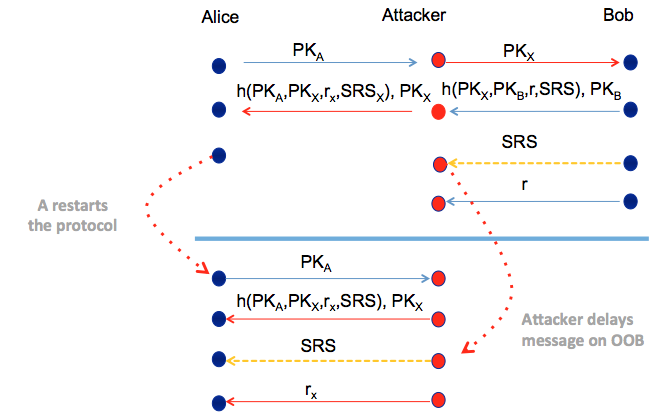
\includegraphics[width=0.8\textwidth]{SRS}
  \caption{Attack Against SRS-AKA Protocol}
  \label{SRSattack}
\end{figure}


\subsection{Attack on Hoepman AKA Protocol}

Since the Hoepman protocol is quite similar to Wong-Stajano protocol with bidirectional channel, the attack found on Wong-Stajano protocol might be used against Hoepman one. But, the difference between two protocols is while two random numbers are exchanged over OOB channel in Wong-Stajano, two short short-hashing values are used in Hoepman version. This apparently lets the attacker a big challenge to break the Hoepman protocol. Nevertheless, due to the less strong hash function, if the attack can find a collision of the short hash function in polynomial time, it is definitely able to launch MITM attack. We take this assumption and present the attack scenario in figure~\ref{Hoepman}, and table~\ref{Hoepmantable}. 
   
\begin{figure}
  \centering
  \includegraphics[width=0.9\textwidth]{Hoepman}
  \caption{Attack Against Hoepman-AKA Protocol}
  \label{Hoepman}
\end{figure}

\begin{table}[t]
\centering
\caption{\textsc{Attack Scenario Against Initiator's Guarantee in Hoepman Protocol}}
\label{Hoepmantable}
{\small
\begin{tabular}{| l | p{11cm} |}
 \hline
 Step 1.1 & Attacker suspends the $S\_h(g^b)$ sent by Bob on OOB channel\\ \hline
 Step 1.2 & Attacker finds $g^x$ so that $S\_h(g^x) = S\_h(g^b)$. It does not necessary to find $h(g^x) = h(g^b)$  \\ \hline
 Step 1.3 & Attacker starts a new session with Alice\\ \hline \hline
 Step 2.1 & Alice sends $h(g^{a2})$ to the Attacker on wireless channel\\ \hline
 Step 2.2 & Attacker sends $h(g^{x})$ to Alice on wireless channel\\ \hline
 Step 2.3 & Attacker drops $S\_h(g_{a2})$ sent by Alice on OOB channel\\ \hline
 Step 2.4 & Attacker releases $S\_h(g^b)$ at Step 1.1 on OOB channel \\ \hline
 Step 2.5 & Alice sends $g^{a2}$ to Attacker on wireless channel \\ \hline
 Step 2.6 & Attacker sends $g^{x}$ to Alice on wireless channel\\ \hline
 Step 2.7 & At the end of the execution, Alice believes she shares a fresh session key with Bob, known actually by the Attacker\\ \hline
\end{tabular}
}
\end{table}

\section{Conclusion}

In this chapter, we have conducted a deep survey on out-of-band channel types and secure device pairing protocols. Moreover, we have provided a novel solution to the fundamental issues of key agreement over a radio links. To our knowledge, our proposal requiring only 2 wireless radio messages and one out-of-band message is more economic than existing protocols in term of communication cost. Yet it still provides a security level equivalent to one of existing protocols. We also gave a sketch of proof in a computational model. Additionally, an implement of our protocol has been conducted and tested in an embedded system to show that it is practical via our benchmark. In mean while, we found some flaws of Wong-Stajano protocols, Hoepman protocol, and SRS-AKA protocol, this has not introduced before. 




 
%% Chapter Template

\chapter{Analysis of Secure Device Pairing Protocols} % Main chapter title

\label{Analysis of Secure Device Pairing Protocols} % Change X to a consecutive number; for referencing this chapter elsewhere, use \ref{ChapterX}

\lhead{Chapter 3. \emph{Analysis of Secure Device Pairing Protocols}} % Change X to a consecutive number; this is for the header on each page - perhaps a shortened title

%----------------------------------------------------------------------------------------
%	SECTION 1
%----------------------------------------------------------------------------------------
Our objective in this chapter is to propose a formalism which models device pairing protocols 
in a natural manner, and permits verification of security properties relevant to these protocols.
We conceive such a formalism as an adaptation of Strand Spaces~\cite{674832}. The model of Strand Spaces is a flexible formalism which represents protocols as a set of local views of participants in a run of a protocol. Taking advantage of this flexibility, our model extends Strand Spaces to deal with OOB channels. Moreover, the attacker model must be refined to take into account the different types of channels, i.e. unsecured channels and OOB channels.

Thank to our improved model, a device pairing protocol with unidirectional out-of-band channel proposed by Wong \& Stajano~\cite{10.1109/MPRV.2007.76} is discovered with a flaw which has not introduced before. More seriously, this protocol is using in current their products such as ~\cite{Stajano:2011aa} and~\cite{Stajano:2014aa}. Ultimately, we produce a procedure which transforms a model of an initial protocol in our extended Strand Spaces to equivalent model of translating protocol without any out-of-band channel in original Strand Spaces model

The chapter 3 begins with some related work. Then we conduct our improved Strand Space to deal with secure channels and device pairing problems. A Wong-Stajano flaw is presented later. Additionally, a proof of our proposed protocol in previous chapter is also offered. At the end of this chapter, our out-of-band translation is presented. 

\section{Related Work}
Whereas a great deal of work tackles problems of formal verification of classical authentication protocols (see for instance~\cite{Ryan:2000:MAS:1407727} for an introduction to the topic), to our knowledge few address problems in cases of multichannel protocols.

Presented in~\cite{jisis11-1-1-07}, a question arises: are auxiliary channels necessary to provide authentication without pre-shared knowledge? Using BAN logic~\cite{Burrows90alogic}, they prove that device authentication using a single channel is not possible . From this analysis, they propose an extension of BAN logic taking into account OOB channels, and using this extension the \textit{Talking to Strangers} protocol from~\cite{Smetters02talkingto} and a simplified version of Wong-Stajano protocol~\cite{10.1109/MPRV.2007.76} were shown to be correct. However, as we will see in subsection~\ref{wong-stajano-protocol}, the Wong-Stajano protocol is vulnerable to an attack. In fact, the proposed formalism does not offer enough expressivity to correctly model the Wong-Stajano protocol.
 
Formal verification of specific versions of Bluetooth protocols has received a lot of attention in literature. Several proposals were introduced to take into account Bluetooth security weaknesses from a version 2.0 to a brand new version 4.0. Some verification tools have been applied such as ProVerif in\cite{Chang_formalanalysis}, and PRISM probabilistic model checker in \cite{Duflot:2006rm}. These work are a first steps towards an automated analysis of formal model of human-assisted protocols. 

\section{Extended Strand Spaces with Out-of-Band Channels}\label{extended-strand}

Due to lack of place, we do not recall here the whole theory of Strand Spaces, but focus on the extensions necessary to examine secure pairing protocols based on Diffie-Hellman scheme. For a complete background on Strand Spaces the reader can consult~\cite{674832},~\cite{Guttman:2002:ATS:568264.568267}, and~\cite{1212716}( we recap the Strand Spaces theory in the appendix~\ref{AppexA}). The extensions mainly concern the algebra and the penetrator model.

Before presenting our extension of Strand Spaces, we formulate some supplementary assumptions concerning the execution of device pairing procedures, that we will have to take into account.
 
\subsection{Model Assumptions}

We now make several practical assumptions in our model as follows: 
\begin{itemize}
\item The hash functions used in the secure device pairing protocol are perfect, that is the attacker cannot perform with success the following attacks: collision attack, pre-image attack, and second-image attack.
\item There is no more than one instance of a particular role uses an OOB channel on each side at a given time.
\item When one device sends the Accept/Reject information, the other device confirms this decision.
\item After a device pairing procedure, the communication session will start later. But in case of no evidence of exchanging procedure, the device pairing procedure replays again with a new session. 
\end{itemize} 

\subsection{Extension to the Algebra}

In the thesis, we will use the term \emph{regular strand} to refer to a run of some legitimate role of a protocol. In the same way, we will use \emph{regular node} to refer to a send or receive event occurring on a regular strand. Additionally, we use \emph{regular behavior} to refer to all regular nodes in a particular run of the protocol.

Our definition of Strand Space algebra is based on the definition from~\cite{1212716}, which adds to model the possibility to deal with DH operation, hash functions, and signatures. To take into account device pairing protocols, we do not need  to consider signatures (neither asymmetric encryption), but must add keyed hash function, or MAC function. We thus redefine the set of terms as follows:

\begin{Definition}
The set of \emph{terms} $\mathcal{A}$ is assumed to be freely generated from four disjoint sets: predictable texts $\mathcal{T}$, unpredictable texts $\mathcal{R}$,  keys $\mathcal{K}$, and Diffie-Hellman values $\mathcal{D}$.

The set of keys $\mathcal{K}$ is divided into two disjoint sets: verification keys $\mathcal{K}_{Ver}$, and keys for symmetric encryption $\mathcal{K}_{Sym}$.

\emph{Compound terms} are built by these operations:
\begin{itemize} 
\item join: $\mathcal{A} \times \mathcal{A} \rightarrow \mathcal{A}$, which represents concatenation of terms. 
\item encr: $\mathcal{K}_{Sym} \times \mathcal{A} \rightarrow \mathcal{A}$, which represents encryption. 
\item DH: $\mathcal{D} \times \mathcal{D} \rightarrow \mathcal{D}$, which represents the Diffie-Hellman operation. We denote the range of DH by $\mathcal{D}_{DH}$.
\item hash: $\mathcal{A} \rightarrow \mathcal{K}_{Sym}$, representing hashing into keys. We denote the range of hash by $\mathcal{K}_{hash}$. 
\item MAC: $\mathcal{K}_{Sym} \times \mathcal{A}  \rightarrow \mathcal{K}_{Sym}$, representing MAC operation with a key into keys.
\end{itemize}
\end{Definition} 

Terms will be denoted by $t, t'$ possibly indexed by an integer. 
The elements from the set of unpredictable or random texts $\mathcal{R}$ are used to play the role of nonces in protocols and will be denoted by $r$ possibly indexed with the identifier of an agent. The elements of $\mathcal{K}$ (resp. $\mathcal{D}$) will be denoted by $k$ (resp. $d$) possibly indexed by an identifier (resp. integer). In the following, $encr(k,t)$, $hash(t)$ and $MAC(k,t)$ will be respectively noted ${\{t\}}_k$, $h(t)$ and $h_k(t)$. The term $join(t,t')$ will be noted $t,t'$. 

In our extension, we will need to explicitly distinguish between different channels. We thus need to define what is a channel.

\begin{Definition}[Channel] A \emph{channel} is a group of strands which can exchange messages in the same region.
\end{Definition} 

One strand may use more than one channel.
For example, given two channels $ch_1$ and $ch_2$ and 3 strands: $A$, $B$, $C$, the strand $A$ and $B$ may use $ch_1$, whereas $B$ and $C$ use $ch_2$. 

If no supplementary assumption is declared, a channel is by default an unsecured public wireless channel. Any specific assumption on a channel, must be specified before formalising the protocol. Since a protocol may use several channels, when sending or receiving a term, the used channel must be specified. The definition of signed term is modified in consequence. 

Since a protocol may use several channels, when sending or receiving a term, the used channel must be specified. The definition of signed term is modified in consequence. 

\begin{Definition}[Signed term]
A \emph{signed term} is a triplet $\langle \delta, t, ch  \rangle$ , noted $\delta_{ch} t$, where $\delta$ is $+$ (sending) or $-$ (reception), $t$ a term, and $ch$ the channel on which $t$ is sent or received.
\end{Definition}

Actually, we will see in subsection~\ref{penetrator_model} that the terms manipulated by a penetrator may receive another sign.
By convention, we will specify the channel only when using an OOB Channel: $-_{ch}t$ means that the term $t$ is received on the OOB channel $ch$, and $-t$ will denote the reception of $t$ on the public wireless channel.

Based on this new definition of signed terms, the definitions of \textit{strand space}, \textit{node}, \textit{edge}, \textit{originating term}, \textit{uniquely originating term}, and \textit{bundle}, \textit{height of a strand} are the same than in~\cite{674832}. 

We refine the notions of \textit{subterm} and \textit{component} from previous works on Strand Spaces as follows.

\begin{Definition}[Subterm]
We say that $t$ is a \emph{subterm} of $t'$, written $t \sqsubseteq t'$ if:
\begin{itemize}
\item $t=t'$ or
\item $t'= (t'_1,t'_2)$ then $t \sqsubseteq t'_1$ or $t \sqsubseteq t'_2$,
\item if $t'={\{t''\}}_k$, then $t \sqsubseteq t''$,
\item if $t'=h(t'')$, then $t \sqsubseteq t''$,
\item if $t'=h_k(t'')$, then $t \sqsubseteq t''$,
\item if $t'=DH(d_1,d_2)$, then $t \sqsubseteq d_1$ or $t \sqsubseteq d_2$
\end{itemize}
\end{Definition}

\begin{Definition}[Component]
We say that a term $t$ is a \emph{component} of term $t'$, written $t \sqsubseteq_c t'$, if $t'$ can be obtained by concatenating $t$ with others terms.
\end{Definition}

For example, the term $(A,g^a,h(A,g^a))$, where $g^a$ denotes a Diffie-Hellman value, contains three components: $A$, $g^a$, and $h(A,g^a)$.

At last, we introduce the notion of boxed term.

\begin{Definition}[Boxed term] 
For a given bundle, we say that a term $t$ is \emph{boxed} at node $n$, if there exists terms $t'$ and $t''$ such that $t \sqsubseteq t'$, $t' \sqsubseteq term(n)$, and $t'$ has one of the following forms: ${\{t''\}}_k$, $h(t'')$, $h_k(t'')$.
\end{Definition}

\subsection{Extended Penetrator Model}\label{penetrator_model}

The new penetrator model must take into account the different kind of channels used in the secure device pairing protocols. Concerning wireless channels, the original Dolev-Yao model~\cite{dolev-yao} is broadened with DH, hash and MAC operations as following:
\begin{itemize}
\item \textbf{F}. Fresh DH value: $\langle +d   \rangle$  where $d \in \mathcal{D}_P$ with $\mathcal{D}_P \subset \mathcal{D}$.
\item \textbf{H}. Hashing: $\langle -t,+h(t)   \rangle$  
\item \textbf{MAC}. MAC: $\langle -t,-k, h_k(t)   \rangle$ where $k$ is a key generated by the attackers. 
\end{itemize} 

As described above, OOB channels intentionally limit penetrator's capacities in term of message manipulation. He is prevented from performing actions on private OOB channels, however, he is still able to realise some actions on public or protected OOB channels. We therefore need specific strands to model actions of penetrators on various types of OOB channels. To do so, we extend signed terms with a new event, $\#_ot$, meaning that penetrators suspend the message $t$ on OOB channel $o$. This brand new event is only adopted for public or protected OOB. Consequently, we extend the penetrator model with following two penetrator traces on OOB channels:

\begin{itemize}
\item \textbf{OVH}. Overhearing : $\langle -_om, +m \rangle$ where $o$ is an OOB channel of type public.
\item \textbf{DRP}. Dropping : $\langle -_om \rangle$.
\item \textbf{SUS}. Suspending : $\langle -_om,\#_om \rangle$ where $o$ is a OOB channel of type long-range public or protected. 
\item \textbf{REL}. Releasing : $\langle \#_om,+_om  \rangle$ where $o$ is a OOB channel of type long-range public or protected.
\item \textbf{RPL}. Replaying : $\langle -_om,+_om,+_om  \rangle$ where $o$ is a OOB channel of type long-range public.
\end{itemize} 

The dropping attack can be modeled by $SUS$ strand without the $REL$ strand. Moreover, $REL$ strand only works for a term $t$ over a public OOB channel $o$ when there exists a $SUS$ strand for $t$ over $o$.  

Having defined the penetrator model, we can now define the notion of revealed term.

\begin{Definition}[Revealed term]
For a given bundle, a term $t$ is called to be $revealed$ at node $n$ if:
\begin{itemize}
    \item $t \sqsubseteq term(n)$, and $t$ can be obtained by the penetrator using his knowledge at node $n$, and
    \item for any $n'$ that precedes $n$ ($n' \preceq n$) such that $t \sqsubseteq term(n')$ the penetrator cannot obtain the $t$ using his knowledge at node $n'$. 
\end{itemize} 
\end{Definition}

\subsection{Pairing Agreement}

Straightforwardly, a goal of secure pairing device protocols is to ensure that two devices with no prior shared knowledge and sharing a common OOB channel, receive the same agreement dataset after acceptance notification. To formalise corresponding security property, we adapt the definition of \textit{agreement property} from~\cite{596782} to our situation.

\begin{Definition}[Agreement Property] We say that a protocol ensures an initiator $A$ \textit{agreement} with a responder $B$ on a set of data items $ds$, if whenever $A$ (acting as initiator) completes a run of a protocol, apparently with responder $B$, then $B$ has previously been running the protocol acting as a responder apparently with A, and each such run of A corresponds to a unique run of B. Furthermore the two agents received the same $ds$ at the end of a run. 
\end{Definition}

A penetrator can attack the protocol if at the end of its run, both devices reach to Accept state, yet having a different agreement dataset. 

\section{Vulnerabilities of Wong-Stajano Protocol}\label{analysisWSP}

This section applies our model to analyse Wong-Stajano Protocol with Unidirectional Channel. Wong and Stajano proposed in~\cite{10.1109/MPRV.2007.76} new mutual authentication and key agreement protocol over bidirectional and unidirectional out-of-band channels. The out-of-band channels ensure data origin authenticity but does not provide confidentiality. Their protocols exploited a short authenticated string over visual channels which provides integrity and data origin authenticity. The Wong-Stajano (WS) Protocol with unidirectional public out-of-band channel is presented in figure~\ref{wong-stajano-protocol}. Its model in our extension of Strand Spaces is defined below.

\begin{figure}[b]
\begin{center}
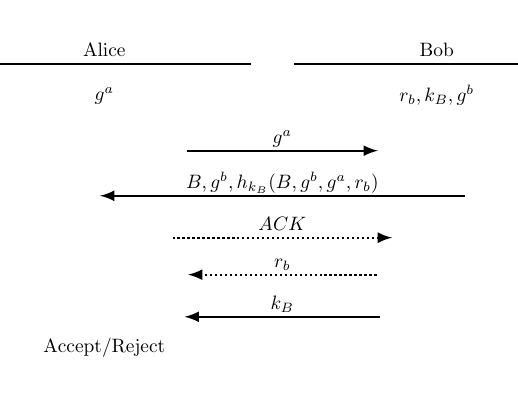
\begin{tikzpicture}[thick,scale=0.7, every node/.style={scale=0.7}]
\matrix (m)[matrix of nodes, column sep=0.1cm,row sep=6mm, nodes={draw=none, anchor=center,text depth=0pt} ]{
Alice & & Bob\\[-4mm]
$g^a$ & & $r_b,k_B,g^b$ \\[-4mm]
& $g^a$ & \\[-4mm]
& $B, g^b, h_{k_B}(B,g^b,g^a,r_b)$ & \\[-4mm]
& $ACK$ & \\[-4mm]
& $r_b$ & \\[-4mm]
& $k_B$ & \\[-4mm]
Accept/Reject & & \\[-4mm]
};

\draw[shorten <=-1.5cm,shorten >=-1.5cm] (m-1-1.south east)--(m-1-1.south west);
\draw[shorten <=-1.5cm,shorten >=-1.5cm] (m-1-3.south east)--(m-1-3.south west);

\draw[shorten <=-1cm,shorten >=-1cm,-latex] (m-3-2.south west)--(m-3-2.south east);
\draw[shorten <=-1cm,shorten >=-1cm,-latex] (m-4-2.south east)--(m-4-2.south west);
\draw[shorten <=-1cm,shorten >=-1cm,-latex,densely dotted] (m-5-2.south west)--(m-5-2.south east);
\draw[shorten <=-1cm,shorten >=-1cm,-latex,densely dotted] (m-6-2.south east)--(m-6-2.south west);
\draw[shorten <=-1cm,shorten >=-1cm,-latex] (m-7-2.south east)--(m-7-2.south west);
 
\end{tikzpicture}
\end{center}
\caption{Wong-Stajano Protocol with Unidirectional Channel} 
\label{wong-stajano-protocol}
\end{figure}

\begin{Definition}
An infiltrated Strand Spaces $(\Sigma,\mathcal{B})$ is a Wong-Stajano protocol space if $\Sigma$ is a union of three kinds of strands:
\begin{itemize}
\item Penetrator strands $s_p \in \mathcal{B}$,
\item "Initiator strand'' with trace $Init[r_b, k_B,g^a,g^b]$ defined to be: \\ 
{\footnotesize $\langle +g^a,-(B, g^b, h_{k_B}(B,g^b,g^a,r_b),+_o ACK,-_{o1}r_b,-k_B \rangle$, where $B \in \mathcal{T}_{name}$, $ACK \in \mathcal{T}$, and $g^a,g^b \in \mathcal{D} \backslash \mathcal{D}_{P}$,}
\item "Responder strand" with traces $Resp[r_b, k_B,g^a,g^b]$ defined to be: \\ {\footnotesize $\langle -g^a,+(B, g^b, h_{k_B}(B,g^b,g^a,r_b)),-_o ACK,+_{o1} r_b,+k_B \rangle$, where $B \in \mathcal{T}_{name}$, $ACK \in \mathcal{T}$, and $g^a,g^b \in \mathcal{D} \backslash \mathcal{D}_{P}$,}
\end{itemize}
with $o$ a short-range public channel and $o1$ a long-range public OOB channel.
\end{Definition}

Unfortunately, agreement property does not hold for the Wong-Stajano protocol. 

\subsection{Responder's Guarantee for Wong-Stajano protocol} 

Responder's guarantee for Wong-Stajano protocol is stated as follows:\\
\textit{Let $\mathcal{B}$ be a bundle containing a strand $st'$ in $Resp[r_b, k_B,g^a,g^b]$ of height 5. If $st'$ uses the channel $o$ in $\langle st',3 \rangle$ and $o1$ in $\langle st',4 \rangle$ , and $r_b, g^b, k_B$ are uniquely originating on $st'$, then $\mathcal{B}$ contains a unique strand $st$ in $Init[r_b, k_B,g^a,g^b]$ of height 5 that also uses channel $o$ and $o1$. Moreover, both strands agree on $g^a,g^b$.}

Proving the responder's guarantee requires to prove following lemmas. Furthermore, these lemmas try to show existing regular( or trusted) nodes in the initiator strand.  

\begin{Lemma}
$r_b$ uniquely originates on $\langle st',2 \rangle$ 
\end{Lemma}
\begin{proof}
Providing that $r_b$ is uniquely originating on $\Sigma$, node $\langle st',2 \rangle $ is a positive node, and $r_b \not\in K$, thus only possibility is that $r_b$ uniquely originates at $\langle st',2 \rangle$ .
\end{proof}

\begin{Lemma}
There exists a regular node $n_4$ in an initiator strand such that $term(n_4) = -_{o1} r_b$.
\end{Lemma}
\begin{proof}
Since the responder strand receives an acknowledgment from Initiator, the initiator apparently has a regular node with term $-_{o1} r_b$. Attacker cannot forge this acknowledgment because it is transmitted on an OOB channel. 
\end{proof}

\begin{Lemma}
There exists a regular node $n_3$ in an initiator strand such that $term(n_3) = -_o ACK$.
\end{Lemma}
\begin{proof}
Because the term of node $\langle st',3 \rangle$ is $-_o ACK$, there is some initiator strand which has a node $n_3$ which term is term $+_o ACK$. The node $n_3$ exploits the same OOB channel $o$ than $\langle st',3 \rangle$.
\end{proof}

Then, to complete the proof of responder's guarantee property, we should prove that:
 
\textit{There exists a regular node $n_2$ in an initiator strand such that} \begin{center}$term(n_2) = -(B, g^b, h_{k_B}(B,g^b,g^a,r_b)$.\end{center}

To prove this, we should show that the term of node $n_2$ cannot be sent from a penetrator strand. It is easy to check for one of following strands: \textit{M, R, S, K, E, D, F, H, MAC}. However we cannot conclude with the \textit{C} strand.

Indeed, using the \textit{C} strand, an attacker may send $(B, g^{x}, h_{k_B}(B,g^{x},g^a,r_b))$ to the initiator strand. 
It supposes that he used before the \textit{MAC} strand by that he knows $k_B$, and $r_b$ which are normally sent after node $\langle st',4 \rangle$. The attacker may have learnt these values in a previous session. Let suppose that in a previous session, the attacker applies the strand $SUS = \langle -_{o1} r_b,\#_{o1} r_b \rangle$ to delay delivery of message to the initiator strand, and then receive $k_B$. If the initiator does not receive the value $r_b$ before expiration time, he will restart a session according to the assumption. In current session, after sending $(B, g^{x}, h_{k_B}(B,g^{x},g^a,r_b))$, the attacker can use $DRP = \langle -_o ACK \rangle$ to drop the ACK message on the OOB channel sent by the initiator. The attacker then executes $REL= \langle \#_{o1} r_b,+_{o1} r_b \rangle$ to deliver the message $r_b$ to the initiator strand. Consequently, the responder's guarantee for Wong-Stajano protocol is not satisfied. Finally, after receiving the $r_b$ message, the new initiator strand verifies MAC value in node $n_2$, then sends the Accept. The attack is successful. Finally, the responder cannot ensure for a regular initiator strand. 


\subsection{Initiator's Guarantee for Wong-Stajano protocol}

Initiator's guarantee for Wong-Stajano protocol is stated as follows:\\
\textit{
Let $\mathcal{B}$ be a bundle containing a strand $st$ in $Init[r_b, k_B,g^a,g^b]$ of height 5. If $st$ uses a public the channel $o$ in $\langle st,3 \rangle$ and $o1$ in $\langle st,4 \rangle$ , and $g^a$ is uniquely originated on $st$, then $\mathcal{B}$ contains a unique strand $st'$ in $Resp[r_b, k_B,g^a,g^b]$ of height 5 that also uses channel $o$ and $o1$. Moreover, both strands agree on $g^a$ and $g^b$.
}

As for the responder's guarantee, the initiator's guarantee does not hold for Wong-Stajano protocol. Trying to prove it leads to the attack scenario detailed in table~\ref{attack-initiator}. 

\begin{table}[t]
\centering
\caption{\textsc{Attack Scenario Against Initiator's Guarantee in Wong-Stajano Protocol with Unidirectional Channel}}
\label{attack-initiator}
{\small
\begin{tabular}{| l | p{11cm} |}
 \hline
 Step 1.1 & Attacker intercepts $g^{a}$ sent by Alice on wireless channel\\ \hline
 Step 1.2 & Attacker replies with $(B, g^{x}, h_{k_X}(B,g^{x},g^a,r_x))$ to Alice on wireless channel\\ \hline
 Step 1.3 & Attacker suspends $r_b$ sent by Bob on OOB channel, and starts a new session with Alice\\ \hline \hline
 Step 2.1 & Alice sends $g^{a'}$ on wireless channel\\ \hline
 Step 2.2 & Attacker responds $(B, g^{x}, h_{k_X}(B,g^{a'},g^{x'},r_b))$ on wireless channel\\ \hline
 Step 2.3 & Attacker drops $ACK$ sent by Alice on OOB channel\\ \hline
 Step 2.4 & Attacker release $r_b$ sent by Bob on OOB channel at Step 1.3\\ \hline
 Step 2.5 & Attacker sends $k_X$ to Alice on Wireless channel\\ \hline
 Step 2.6 & At the end of the execution, Alice believes she shares a fresh session key with Bob, known actually by the Attacker\\ \hline
\end{tabular}
}
\end{table}


\section{Analysic of 2-Move Secure Device Pairing Protocol}\label{chap42move}

We assume that:
\begin{itemize}
\item Participants reuse their public keys across protocol sessions. 
\item Hash function using in the first A's message is perfect. 
\item Keyed hash function is simplified as a generic hash function exclusive-or with a key. And it is considered as a weaker version than the generic version used in the first message. 
We light this assumption since length of output of keyed hashed functions is usually short over authentic channels. Therefore, attackers could exploit this weakness. 
\end{itemize}

Our protocol is modelled as follows. 

\begin{Definition}
An infiltrated Strand Spaces $(\Sigma,\mathcal{B})$ is the protocol space if $\Sigma$ is a union of three kinds of strands:
\begin{enumerate}
\item Penetrator strand $s_p \in \mathcal{P}$,
\item "Initiator strand'' with trace {\small $Init[g^a,g^b,r_a,r_b]$} defined to be: \\ 
 {\small $\langle +(g^a,h(g^a,r_a)),-(g^b,r_b),+_o(r_a \otimes h_{r_b}(g^a,g^b))$, \\ where $g^a,g^b \in \mathcal{B} \backslash \mathcal{P}$,}
\item "Responder strand'' with trace\\
 {\small $Resp[g^a,g^b,r_a,r_b]$} defined to be: \\ 
 {\small $\langle -\{g^a,h(g^a,r_a)\},+\{g^b,r_b\}, -_o(r_a \otimes h_{r_b}(g^a,g^b))$, \\ where $g^a,g^b \in \mathcal{B} \backslash \mathcal{P}$,}
\end{enumerate}
with $o$ a long-range public OOB channel.
\end{Definition}

We now proceed with showing correctness of our protocol by both proving initiator and responder guarantees.

\subsubsection{Initiator's Guarantee}

\begin{Proposition}
Let $\Sigma$ be a Strand Spaces of the protocol, and $\mathcal{B}$ a bundle containing an initiator's strand $st$ with trace $Init[g^a,g^b,r_b,r_a]$ of height 3. If
 \begin{itemize}
 \item $g^a,g^b \not\in D_P$, and $g^a \not= g^b$, and
 \item $r_a,r_b$ uniquely originate in $\Sigma$, and $r_a \not= r_b$,
 \end{itemize}
then $\mathcal{B}$ contains a responder strand $st'$ with trace $Resp[g^a,g^b,r_a,r_b]$. Both strands agree on $g^a$ and $g^b$.
\end{Proposition}

\begin{proof}
Basically, a proof proceeds according to following steps: at first we locate where $r_a$ originates, and after that, we need to guarantee that all nodes in unique Responder's strand are regular.
 If any single node cannot be proved, the proof will fail. 
These steps are detailed in lemmas \ref{lemme4.2} to \ref{lemme4.6} below.
\end{proof}

\begin{Lemma}\label{lemme4.2}
$r_a$ uniquely originate at $\langle st,1 \rangle$ 
\end{Lemma}

\begin{proof}
Since $r_a$ uniquely originates in $\Sigma$, and node $\langle st,1 \rangle$ is a positive node and the first node of strand $st$, then no strand other than $st$, can emit these terms. Therefore, $r_a$ must originate at $\langle st,1 \rangle$.
\end{proof}

\begin{Lemma}\label{lemme4.3}
There is a regular node $n_3$ such that $term(n_3)= -_o(r_a \otimes h_{r_b}(g^a,g^b))$ on a responder strand. 
\end{Lemma}

\begin{proof}
Since $term(\langle st,3 \rangle) = +_o(r_a \otimes h_{r_b}(g^a,g^b))$, only a regular responder strand can use the channel $o$ to receive this message. Let call $n_3$ the node which receives $(r_a \otimes h_{r_b}(g^a,g^b))$, and $n_3$ belongs to some $Resp[*,g^b,*,r_b]$.
\end{proof}

Note that, $g^b$ and $r_b$ could be sent from the attacker, hence let assume that B receives $(r_a \otimes h_{r_{xb}}(g^a,g^{xb}))$ in which $r_{xb}$ and $g^{xb}$ are sent from the attacker. Moreover, in case $n_3 \in SUS$, then the attacker would get $r_a$ and $r_b$ at this step. We will check them in following lemmas. 

\begin{Lemma}\label{lemme4.4}
There is a regular node $n_1$ such that $term(n_1)= -(g^a,h(g^a,r_a))$ on a responder strand. 
\end{Lemma}

\begin{proof}
Following the proof of lemma~\ref{lemme4.3}, the responder verifies the committed value at $n_1$ using $r_a$ extracted in $n_3$. If the verification fails, the responder shows a Reject status immediately. 

The responder calculates $r'_{a} = (r_a \otimes h_{r_{xb}}(g^a,g^{xb})) \otimes (h_{r_b}(g^{xa},g^b))$ where $r_{xa},r_{xb}$ and $g^{xa},g^{xb}$ are created by some attackers. 
From the assumption on keyed hash functions, $r'_{a} = (r_a \otimes r_b \otimes r_{xb} \otimes h(g^a,g^{xb}) \otimes h(g^{xa},g^b))$ (1).

From following facts,
\begin{description} 
 \item [(i)] $r_a$ is revealed after seeing $r_{xb}$, 
 \item [(ii)] $r_{xb}$ is committed in $\langle st,2 \rangle$ just after $\langle st,1 \rangle$, and $r_{xa}$ is committed before knowing $r_b$, 
 \item[(iii)] $r_a$ and $r_b$ uniquely originate in $\Sigma$, 
 \item [(iv)] hash functions are perfect,
\end{description}
we can deduce that attackers have not ability to generate such $r'_{a}$ in (1) before $n_1$. 
Since $n_1$ maps to the first node of some responder strand $st'$ in which $r_b$ belongs, $n_1$ must be a regular node. 
\end{proof}

\begin{Lemma}\label{lemme4.5}
There is a regular node $n_2$ such that $term(n_2)= + (g^b,r_b))$ on a responder strand. Moreover, $n_1 \preceq n_2 \preceq n_3$.
\end{Lemma}

\begin{proof}
Using results of lemmas ~\ref{lemme4.3} and ~\ref{lemme4.4}, we have two regular nodes $n_1$ and $n_3$ in some responder strands $Resp[*,g^b,*,r_b]$. In fact, there is a regular node $n_2$ with $term(n_2)= + (g^b,r_b))$ such that $n_1 \preceq n_2 \preceq n_3$. 
\end{proof}

\begin{Lemma}\label{lemme4.6}
Both participants agree on $g^a$ and $g^b$. 
\end{Lemma}

\begin{proof}
For arbitrary Alice, Bob and $r_a$, if strand $st' \in Resp[g^a,g^b,r_a,r_b]$, then sign of $\langle st',2 \rangle$ is positive. Moreover, according to two previous lemmas, there is a relationship $n_1 \preceq n_2 \preceq n_3$. When $r_b \sqsubseteq term(\langle st',2 \rangle )$, there is at most one such $st'$.

Now, let check if $g^a$ actually originates on $st$ or not. Since $g^a$ stays in the same box with $r_a$ at $\langle st,1 \rangle$, the attacker cannot produce a term corresponding to $term(\langle st,1 \rangle )$ with a fake $g^{x}$. Therefore, $g^a$ must originate on $st$. 

Using the same argument, since $g^b$ and $r_b$ stay in the same box at $n_3$, and $r_b$ uniquely originates in $\Sigma$, the initiator receives the correct $g^b$.
\end{proof}

So the protocol satisfies injective agreement for the initiator~A. 


\subsection{Responder's Guarantee }

\begin{Proposition}
Let $\Sigma$ be a Strand Spaces of the protocol, and $\mathcal{B}$ be a bundle containing a responder's strand $st'$ with trace $Resp[g^a,g^b,r_a,r_b]$ of height 3. If
\begin{itemize}
\item $g^a,g^b \not\in D_P$, and $g^a \not= g^b$, and
\item $r_a,r_b$ uniquely originate in $\Sigma$, and $r_a \not= r_b$.
\end{itemize}
Then $\mathcal{B}$ contains an initiator strand $st$ with trace $Init[g^a,g^b,r_a,r_b]$. Both strands agree on $g^a$ and $g^b$.
\end{Proposition}

\begin{proof}
The proof of Responder's guarantee is nearly identical to Initiator's guarantee proof. We need to verify that all nodes in a unique $Init[g^a,g^b,r_a,r_b]$ are regular. Firstly, we need to locate $r_b$. These steps are detailed in lemmas \ref{lemme4.9} to \ref{lemme4.13} below.
\end{proof}

\begin{Lemma}\label{lemme4.9}
$r_b$ originates at node $\langle st',2 \rangle$ .
\end{Lemma} 

\begin{proof}
$r_b$ is a subterm of the positive node $\langle st',2 \rangle$, thus it could lie on $\langle st',1 \rangle$. However, according to the assumption, $r_b$ is neither $g^a$ nor $h(r_a,g^a)$, and $r_b$ uniquely originates in $\Sigma$, then $r_b$ must originate at $\langle st',2 \rangle$.
\end{proof}
 
\begin{Lemma}\label{4.10}
There is a regular node $n_3$ such that $term(n_3)= +_o(r_a \otimes h_{r_b}(g^a,g^b))$ 
\end{Lemma}

\begin{proof}
Since the responder must receive an authenticated message over $o$ before notifying an Accept/Reject status, it means that some initiator has sent a message on a channel $o$. Therefore, let call $n_3$ with $term(n_3)= +_o(r_a \otimes h_{r_b}(g^a,g^b))$. Even if $n_3$ is on a $SUS$ or $REL$ strand, its value is not modified due to the reception on OOB channel. Consequently, there is a regular initiator strand $st \in Init[g^a,*, r_a,*]$ such that $n_3 \in st$. 
\end{proof}

We note that $r_b$ and $g^b$ could be generated by some penetrator strands. Suppose that the responder receives $r_{xb}$ instead of $r_b$, and $g^{xb}$ instead of $g^b$. So the $term(n_3)$ could be $+_o(r_a \otimes h_{r_{xb}}(g^a,g^{xb}))$.

\begin{Lemma}\label{4.11}
There is a regular node $n_1$ such that $term(n_1)= +(g^a,h(g^a,r_a))$.
\end{Lemma}

\begin{proof}
Assume that $n_1$ resides on some attackers, and $term(n_1) = +(g^{xa},h(g^{xa},r_{xa}))$ where $g^{xa}$ and $r_{xa}$ are generated by an attacker. According to last analysis in lemma ~\ref{4.10}, $n_3$ could lay on $SUS$ and be reused in another session against the responder. 

Now the responder calculates $r'_{a} = (r_a \otimes h_{r_{xb}}(g^a,g^{xb}) \otimes (h_{r_b}(g^{xa},g^b))$, then checks if $h(g^{xa},r'_{a})$ equals $h(g^{xa},r_{xa})$ or not. 

We have,
\begin{description} 
 \item [(i)] $r_a, r_b$ uniquely originate on $\Sigma$, 
 \item [(ii)] $r_{xa}$ is submitted before $\langle st',2\rangle$, 
 \item [(iii)] $r_{a}$ is revealed only in $\langle st',3 \rangle$, 
 \item [(iv)] hash functions are perfect, 
\end{description}
hence the attacker has no way to create such $r_{xa}$ before $\langle st',2 \rangle$ where $r_b$ originates. Therefore, $n_1$ is regular node. 
 \end{proof}

\begin{Lemma}\label{4.12}
There is a regular node $n_2$ such that $term(n_2)= -(g^b,r_b))$, and $n_1 \preceq n_2 \preceq n_3$.
\end{Lemma}

\begin{proof}
According to the lemmas ~\ref{4.10} and~\ref{4.11}, we have some regular strands $st \in Init[g^a,*, r_a,*]$ such that $n_1, n_3 \in st$. 
Hence, $st$ must contain $\langle st,2 \rangle$ labeled as $n_2$ with $term(n_2)= -(g^b,r_b))$. Finally, we have $n_1 \preceq n_2 \preceq n_3$.
\end{proof}

\begin{Lemma}\label{lemme4.13}
Both participants agree on $g^a$ and $g^b$. 
\end{Lemma}

\begin{proof}
For arbitrary Alice, Bob and $r_b$, if strand $st \in Init[g^a,g^b,r_a,r_b]$, then signs of $\langle st,1 \rangle$ and $\langle st,3 \rangle$ are positive. Moreover, according to previous lemmas, relationship $n_1 \preceq n_2 \preceq n_3$ holds. When $r_a \sqsubseteq term(\langle st,1 \rangle )$, there is at most one such $st$.

Now, let check if $g^a$ actually originates on $st$ or not. Since $g^a$ stays in the same box with $r_a$ at $\langle st,1 \rangle$, the attacker cannot produce a term corresponding to $term(\langle st,1 \rangle )$ with a fake $g^{x}$. Therefore, $g^a$ must originate on $st$. 

Using the same argument, since $g^b$ and $r_b$ stay in the same box at $n_3$, and $r_b$ uniquely originates in $\Sigma$, the initiator receives the correct $g^b$.
\end{proof}

So the protocol satisfies injective agreement for the responder~B. 

\section{Analysis of Commitment Schemes}

As introduced chapter 2, modern secure device pairing protocols usually take advantage of commitment schemes to provide provable security. Hence, we generalise and model commitment schemes in our formalisation to offer a useful tool to process commitment-based device pairing protocols quickly. To do that, we at first define a commitment scheme such that when it is recognised in a protocol, it straightforwardly results two regular strands. 

\subsection{Formalism of Commitment Schemes}

To begin with, we define a commitment scheme as follows. 
 
\begin{Definition}[Commitment Scheme]
A commitment scheme $CS(r_a,r_b)$ for a random pair $(r_a,r_b)$ in which $r_a \not= r_b$ contains one of these strands:
\begin{itemize}
\item \emph{3-Move strand}: $+c(r_a) \Rightarrow -(r_b) \Rightarrow +d(r_a)$;
\item \emph{4-Move strand}: $+c(r_a) \Rightarrow -c(r_b) \Rightarrow+d(r_a) \Rightarrow -d(r_b) $ .
\end{itemize}
\end{Definition}

The generic device pairing protocol is modelled as follows. 

\begin{Definition}
An infiltrated Strand Spaces $(\Sigma,\mathcal{B})$ is the device protocol space if $\Sigma$ is a union of three kinds of strands:
\begin{enumerate}
\item Penetrator strand $s_p \in \mathcal{B}$,
\item "Initiator strand'' with trace {\small $Init[r_a,r_b]$},
\item "Responder strand'' with trace {\small $Resp[r_a,r_b]$},
\end{enumerate}
with a public OOB channel $o$, $r_a$ and $r_b$ are random numbers. 
\end{Definition}

\begin{Proposition}[Provable Bundle]\label{provablebundle}
Let $\mathcal{B}$ be a bundle of a secure pairing protocol using an out-of-band channel $o$ in which:
\begin{itemize}
\item a regular random pair $(r_a,r_b)$ uniquely originates in $\mathcal{B}$, and $r_a \not= r_b$;
\item a commitment scheme $CS(r_a,r_b)$ is found in $\mathcal{B}$;
\item a function $f(r_a,r_b)$ is second-preimage resistant;
\end{itemize}
If the output of $f$ is transferred over an out-of-band channel $o$ between two regular principals, there exist two unique regular strands $st$ and $st'$ in $\mathcal{B}$ using $f$ such that $r_a \in st$ and $r_b \in st'$. Moreover, both strands agree on $(r_a,r_b)$. 
\end{Proposition}

\begin{proof}

Since $o \in \mathcal{B}$, there exist at least two different strands sharing $o$. Let call two strands be $st$ and $st'$, and $term(\langle st,i\rangle )=+_o(f)$, and $term(\langle st',j\rangle ) = -_o(f)$. Generally, we can assume that $st$ is Initiator and $r_a \in st$, $st'$ is Responder and $r_b \in st'$. 

\emph{Initiator Guaranty}: As described above, a regular node $\langle st',j\rangle $ associates to $o$ such that $term(\langle st',j\rangle ) = -_o(f)$. We assume that when the protocol finishes, $st$ gets $f(r_a,r_{x2})$, $st'$ gets $f(r_{x1},r_b)$ where $r_{x1}$ and $r_{x2}$ could be generated by attackers. Then, $f(r_a,r_{x2})$ must equal $f(r_{x1},r_b)$ since they are transfered via $o$. 

Observing that $X$ has to submit $r_{x2}$ before actually knowing $r_a$. Similarly, $X$ has to submit $r_{x1}$ before actually seeing $r_b$. Thus irrespectively of the attacking strategy taken by $X$, $r_a$ and $r_b$ will be revealed after $r_{x1}$ and $r_{x2}$ have been generated and submitted. If it happens that both $r_a$ and $r_b$ are revealed in the same time, then we can pick an arbitrary one. 

Assume that $r_a$ is revealed after $r_b$, we have:
\begin{description}
 \item [(i)] $r_a$ and $r_b$ are independently and uniformly distributed random variables, 
 \item [(ii)] $r_{x1}$ and $r_{x2}$ must be generated and submitted before either $r_b$ or $r_a$ are revealed, 
 \item [(iii)] each principal can open at most $\gamma$ sessions. 
 \item [(iv)] there are $n$ participants in the network. 
 \item [(v)] $m_{x1}$ and $m_{x2}$ are possibly unchanged.
 \item [(vi)] $f$ is second-preimage resistant. 
\end{description}
The same holds for the case where $r_b$ is revealed after $r_a$. Therefore, $Pr[f(r_a,r_{x2}) = f(r_{x1},r_b)] \leq n.\gamma.2^{-k}$, where $k$ is the length of $r_a$ or $r_b$. When $k$ is sufficiently large, the attack is impossible. 

As consequence, the protocol satisfies the agreement on $(r_a,r_b)$ for the Initiator. 

\emph{Responder Guaranty} is quite identical to Initiator guaranty. 

Finally, $\mathcal{B}$ is provable. 
\end{proof}

\subsection{An Example}
Let's take a simple example. The protocol presented at the figure~\ref{dataagreel} aims to provide a data agreement between two participants. The protocol happens as follows.
\begin{enumerate}
\item Alice picks a random value $r_a$. Bob picks a random value $r_b$
\item Alice sends $m,h(m,r_a)$ to Bob.
\item Bob sends $r_b$ to Alice.
\item Alice sends $r_a$ to Bob.
\item Alice sends $h(r_a,r_b,m)$ to Bob over a long-range public out-of-band channel. 
\item Bob verifies the received value and announces the result to Alice. 
\item Alice confirms by pushing an Accept button. 
\end{enumerate}

\begin{figure}[b]
\begin{center}
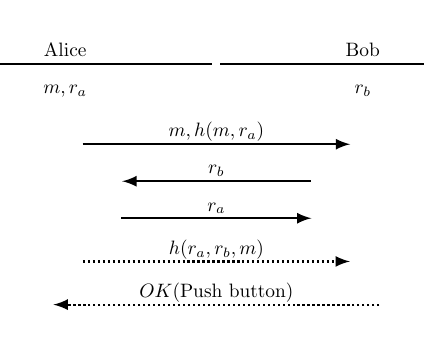
\begin{tikzpicture}[thick,scale=0.7, every node/.style={scale=0.7}]
\matrix (m)[matrix of nodes, column sep=0.5cm,row sep=6mm, nodes={draw=none, anchor=center,text depth=0pt} ]{
Alice & & Bob\\[-4mm]
$m,r_a$ & & $r_b$ \\[-4mm]
					 &$m,h(m,r_a)$ & \\[- 4mm]
						& $r_b$ & \\[- 4mm]
						& $r_a$ & \\[- 4mm]
						& $h(r_a,r_b,m)$ & \\[- 4mm]
& $OK$(Push button) & \\[-4mm]
};

\draw[shorten <=-1.5cm,shorten >=-1.5cm] (m-1-1.south east)--(m-1-1.south west);
\draw[shorten <=-1.5cm,shorten >=-1.5cm] (m-1-3.south east)--(m-1-3.south west);

\draw[shorten <=-1cm,shorten >=-1cm,-latex] (m-3-2.south west)--(m-3-2.south east);
\draw[shorten <=-1cm,shorten >=-1cm,-latex] (m-4-2.south east)--(m-4-2.south west);
\draw[shorten <=-1cm,shorten >=-1cm,-latex] (m-5-2.south west)--(m-5-2.south east);

\draw[shorten <=-1cm,shorten >=-1cm,-latex,densely dotted] (m-6-2.south west)--(m-6-2.south east);
\draw[shorten <=-1cm,shorten >=-1cm,-latex,densely dotted] (m-7-2.south east)--(m-7-2.south west);

\end{tikzpicture}
\end{center}
\caption{A Simple Data Agreement Protocol} 
\label{dataagreel}
\end{figure}

The protocol is modelled as follows. 

\begin{Definition}
An infiltrated Strand Spaces $(\Sigma,\mathcal{B})$ is the protocol space if $\Sigma$ is a union of three kinds of strands:
\begin{enumerate}
\item Penetrator strand $s \in \mathcal{P}$,
\item "Initiator strand'' with trace {\small $Init[r_a,r_b,m]$} defined to be: \\ 
 {\small $\langle +(m,h(m,r_a)),-r_b,+r_a,+_o(h(r_a,r_b,m))$}
\item "Responder strand'' with trace {\small $Resp[r_a,r_b,m]$} defined to be: \\ 
 {\small $\langle -(m,h(m,r_a)),+r_b,-r_a,-_o(h(r_a,r_b,m))$}
\end{enumerate}
with a long-range public OOB channel $o$ and a second-preimage resistance function $h$. 
\end{Definition}

\begin{Proposition}
Let $\Sigma$ be a Strand Spaces of the protocol, and $\mathcal{B}$ a bundle containing an initiator's strand $st$ with trace $Init[r_a,r_b,m]$ of height 4. If $r_a,r_b$ uniquely originate in $\Sigma$, and $r_a \not= r_b$, then $\mathcal{B}$ contains a responder strand $st'$ with trace $Resp[r_a,r_b,m]$. Moreover, both strands agree on $r_a$, $r_b$ and $m$.
\end{Proposition}

\begin{proof}
Intuitively, $\mathcal{B}$ contains a $3-Move$ commitment scheme $CS(r_a,r_b)$ with a function $h(r_a,r_b,m)$. According to the proposition~\ref{provablebundle}, $\mathcal{B}$ is a provable bundle in which there are two unique regular strand $st$ and $st'$ such that $r_a \in st$, and $r_b \in st'$. Furthermore, due to well partial-ordered relationship in $st'$, $st'$ has a height 4. 

Since $m \sqsubseteq term( \langle st,4 \rangle) = h(r_a,r_b,m)$, $m$ is ensured for data origin authentication. As a result, $st'$ receives a correct $m$ after the protocol. Finally, $st$ and $st'$ agree on $m$.
\end{proof}

\section{Out-of-band Channel Transformation}

We aim in this section to propose a translation procedure that transforms a model in our previous formalism of an initial protocol with OOB channels into a model in original Strand Spaces of a protocol that does not use any OOB channel while preserves security properties of initial protocol: if there is no attack against a transformed model there is no attack against an initial model. As a result, a protocol using OOB channels can now be verified using a security protocol analyzer such as~\cite{596779} or~\cite{BlanchetCSFW01}.

\subsection{Related Work}
To our knowledge, out-of-band security property is only partially addressed in existing work. Most of existing methods only deal with private or protected channels and simulate use of these out-of-band channels via a set of pre-shared or public keys, for example in \cite{Diaz2014149}, \cite{Han:2014:SPM:2627393.2627400}, and \cite{Bella:2003aa}.

Our approach is similar to Gavin Lowe and al. approach in~\cite{cdilloway2007spec} and \cite{Kamil:2011aa}. In these studies, they specified specifications of secure channels that are provided when using secure transport protocols. Properties include confidentiality, no faking, no hijacking, and no redirecting. Then, the authors illustrated them via some cryptographic protocols using a set of private and public keys, but did not prove security of these protocols. This work are implemented in Casper/FDR verification tool\cite{596779}. Basically, the differences between this work and ours are (i) they only consider transport layer while we can take into account both physical layer and transport layer, (ii) we provide a specific model of penetrator's abilities on OOB channel while they limit penetrator's abilities on secure channels, and (iii) we provide some method to prove security of a protocol.

Another security protocol verification tool, Proverif \cite{BlanchetCSFW01}, integrates out-of-band channels.
There are two kinds of channels formalised in Proverif: \emph{public} and \emph{private}. Attacker can overhear on a public channel, whereas they cannot do anything on a private channel. Penetrator's capabilities are thus more limited than in our model.

\subsection{Channel Property Transformation}\label{OOB-transform}
The idea of the translation is simulating all security properties offered by each out-of-band channel by equivalent ones fully constructed by cryptographic primitives. Firstly we state underlying assumptions:

\begin{description}
\item [(A1)] All regular participants are honest. 
\item [(A2] All regular participants have pre-shared their identities, public keys, or pre-shared secret keys. 
\item [(A3)] All regular keys are not known by any penetrator. 
\item [(A4)] Each honest participant runs one instance of the protocol at a time. 
\end{description}

We adopt following notations: 
\begin{itemize}
\item $m$ is a desired sharing data. 
\item $r_a$, $r_b$ are nonces (pseudo-random numbers) respectively generated by $A$ and $B$. 
\item $Pr_I$ is a private key of entity $I$, $Pb_I$ is a public key of entity $I$. 
\item $i$ is an integer number corresponding to an index of an out-of-band message in an original protocol. 
\item $h$ is a hash function. 
\item $A,B$ are names of participants. 
\item $\mathcal{B}^{SP}_o(m,i)$ is a shape modelled in original Strand Spaces providing an agreement property for data $m$. 
\item $sk^r_o(m,i)$ is a Initiator skeleton, and $sk^r_o(m)$ is a Responder skeleton in $\mathcal{B}(m,i)$. 
\end{itemize}

To implement this idea, we introduce four specific cryptographic shapes~\footnote{Definitions of shape and skeleton are defined at~\cite{Doghmi:2007:SHS:1230146.1230260}}, or sub-bundle $\mathcal{B}^{SP}_{o}(m,i)$ containing a sending skeleton $sk^e_o(m)$, and a receiving skeleton $sk^r_o(m)$, offering the same security quality as $*_o()$ does.

In these shapes, Alice ($A$) and Bob ($B$) wish to agree on a message $m$. Attackers win if one of two participants gets different $m$. 

To provide data origin authentication, a hash of $m$ is encrypted by a public or private key. Data confidentiality is offered by a pair of public and private keys. Keys are apparently assumed to not belong to any attacker. 

Following definition allows characterising a fact that a principal receiving a message is able to access to a given subterm of this message. In particular, if this subterm is encrypted the principal own requires keys to decrypt, and this subterm is not masked by a non-inversible function (hash or keyed-hask function). 

\begin{Definition}[Extractable]
$m$ is called \emph{extractable} from $m'$, presented as $m \sqsubseteq^K_{ex} m'$, if $m \sqsubseteq m'$, and $m$ is obtained by applying a limited number of operations of splitting and decryption with a set of keys $K$ into $m'$.
\end{Definition}

%Model of a long-range public channel
\subsubsection*{Model of a long-range public channel in original Strand Spaces}\label{longrange}

Let $\mathcal{B}^{SP}_{lrp}(m,i)$ be a shape in the classical Strand Spaces pictured in figure~\ref{protocol1} . $\mathcal{B}^{SP}_{lrp}(m,i)$ provides data origin authentication on $m$ for Responder as a long-range public channel does. In this scheme, $\{h(m)\}_{Pr_a}$ protected under $Pb_B$ will ensure integrity of the message. Hence, Responder can ensure the the origin of message by using the corresponding Initiator public key. 

\begin{figure}
\begin{center}
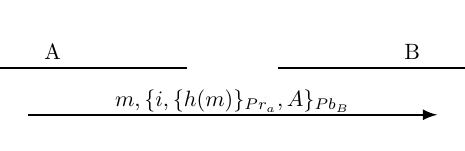
\begin{tikzpicture}[thick,scale=0.8, every node/.style={scale=0.8}]
\matrix (m)[matrix of nodes, column sep=0.5cm,row sep=6mm, nodes={draw=none, anchor=center,text depth=0pt} ]{
A & & B \\[-4mm]
 & $m, \{i,\{h(m)\}_{Pr_a},A\}_{Pb_B}$ & \\[-4mm]
};

\draw[shorten <=-1.5cm,shorten >=-1.5cm] (m-1-1.south east)--(m-1-1.south west);
\draw[shorten <=-1.5cm,shorten >=-1.5cm] (m-1-3.south east)--(m-1-3.south west);
\draw[shorten <=-1cm,shorten >=-1cm,-latex] (m-2-2.south west)--(m-2-2.south east);
\end{tikzpicture}
\end{center}
\caption{Shape 1} 
\label{protocol1}
\end{figure}

\begin{Proposition}
Considering assumptions (A1) to (A4), the shape $\mathcal{B}^{SP}_{lrp}(m,i)$ containing two skeletons $sk^e_{lrp}(m,i)$ and $sk^r_{lrp}(m,i)$ holds data origin authentication for $m$. 
\end{Proposition}

\begin{proof}

\emph{Initator's guarantee}: Since the initiator’s keys are not owned by any attacker, Initiator's messages cannot be forged. Additionally, $m$ signed by the initiator's private key, and extractable by a responder's private key. Therefore, initiator skeleton $sk^e_{lrp}(m,i)$ hold data origin authentication for Initiator. Note that, attackers can drop messages, but Initiator goals are still satisfied. 

\emph{Receiver's guaranty}: Using the unsolicited test~\cite{Guttman:2002:ATS:568264.568267} for uncompromised keys, the receiver skeleton is able to verify existence of the regular node on the initiator skeleton. Data origin authentication of $m$ is obtained in the hash value covered by the initiator's private key. $m$ is apparently extractable. Finally, the responder skeleton $sk^r_{lrp}(m,i)$ holds its goals. 
 \end{proof}

%Model of a short-range public channel
\subsubsection*{Model of a short-range public channel in original Strand Spaces}\label{shortrange}

We simulate a non-suspend channel by a unique instance of a initiator and a corresponding receiver for each specific out-of-band message. Precisely, in our proposed scheme, each side can ensure the unique execution of the other side. As the result of that, when a message is revealed, an attacker cannot reuse it in other sessions. 

Let $\mathcal{B}^{SP}_{srp}(m,i)$ the shape displayed at figure~\ref{protocol2} modelling in the original Strand Spaces. $\mathcal{B}^{SP}_{srp}(m,i)$ offers data origin authentication, non-replaying attack against Responder, and unique execution of each participant in each protocol session. As a consequence, $\mathcal{B}^{SP}_{srp}(m,i)$ provides all security properties as a short-range public out-of-band channel does. Additionally, we let $r_a$ visible to attackers purposely, because we allow dropping attack. By this way, attackers can produce the second message to obtain $m$, but definitely cannot reuse it. 

We use a commitment scheme to keep away replaying attack. $A$ firstly commits a value $h(m,r_a)$, then releases $m$ after receiving a random challenge $r_b$ from $B$. Although an attacker may produce a fake second message to obtain $m$, $B$ is still able to verify the fresh of $m$ by checking the value of $r_b$ and $r_a$ used in current session with $A$. $r_b$ apparently is known only by $A$ as encrypted by the $A$'s public key. Meanwhile, the last message like one in $\mathcal{B}^{SP}_{lrp}(m,i)$ offers data origin authentication. 


\begin{figure}
\begin{center}
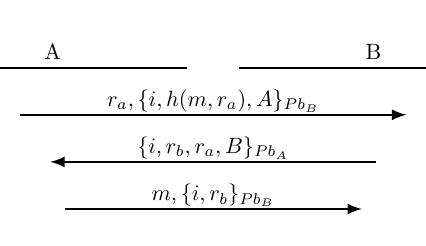
\begin{tikzpicture}[thick,scale=0.8, every node/.style={scale=0.8}]
\matrix (m)[matrix of nodes, column sep=0.4cm,row sep=6mm, nodes={draw=none, anchor=center,text depth=0pt} ]{
A & & B\\[-4mm]
 & $r_a,\{i,h(m,r_a),A\}_{Pb_B}$ & \\[-4mm]
 & $\{i,r_b,r_a,B\}_{Pb_A}$ & \\[-4mm]
 & $m,\{i, r_b\}_{Pb_B}$ & \\[-4mm]
};

\draw[shorten <=-1.5cm,shorten >=-1.5cm] (m-1-1.south east)--(m-1-1.south west);
\draw[shorten <=-1.5cm,shorten >=-1.5cm] (m-1-3.south east)--(m-1-3.south west);
\draw[shorten <=-1cm,shorten >=-1cm,-latex] (m-2-2.south west)--(m-2-2.south east);
\draw[shorten <=-1cm,shorten >=-1cm,-latex] (m-3-2.south east)--(m-3-2.south west);
\draw[shorten <=-1cm,shorten >=-1cm,-latex] (m-4-2.south west)--(m-4-2.south east);
\end{tikzpicture}
\end{center}
\caption{Shape 2} 
\label{protocol2}
\end{figure}

\begin{Proposition}
Considering assumptions (A1) to (A4), $\mathcal{B}^{SP}_{srp}(m,i)$ containing two skeletons $sk^e_{srp}(m,i)$ and $sk^r_{srp}(m,i)$ holds data origin authentication, and unique execution of each sides. 
\end{Proposition}

\begin{proof}

\emph{Initator's guarantee}: Since the initiator’s keys are not owned by any attacker, the third message cannot be forged. Hence, data origin authentication of $m$ is ensured in the message received by the responder. Moreover, $m$ is clearly extractable by the responder's private key. 
We also obviously have a outgoing test edge $\langle sk^e_{srp}(m,i),1 \rangle \Rightarrow \langle sk^e_{srp}(m,i),2 \rangle$ for a nonce $r_a$. Initiator ensures the existence of the responder, but it could be an attacker. Nevertheless, according to our assumption on uncompromised keys, and unique origination of $r_b$, Initiator knows attackers cannot forge or reuse the third message. Finally, the initiator skeleton holds the unique execution of Responder and data origin authentication.

\emph{Responder's guarantee}: Firstly, $m$ is extractable in third message by the responder's private key. Since the private key $Pr_a$ does not belong to attacker’s keys, attacker cannot generate the third message. 

According to following reasons: 
\begin{enumerate}
\item[(i)] Using the authentication test 2~\cite{Guttman:2002:ATS:568264.568267} for $r_b$, the responder is able to verify existence of the two last regular nodes of an initiator skeleton.
\item[(ii)] Additionally, uniquely origination of $r_a$ allows $B$ to ensure for the unique initiator.
\item [(iii)] Data origin authentication of $m$ is secured by the hash value signed by the initiator's private key. 
\end{enumerate}

Responder skeleton $sk^r_{srp}(m,i)$ holds unique execution of Initiator and data origin authentication.
 \end{proof}

%Model of a protected public channel
\subsubsection*{Model of a protected channel in original Strand Spaces}\label{protect}

Let be $\mathcal{B}^{SP}_{pro}(m,i)$ a shape described at figure~\ref{protocol3} which offers data confidentiality of $m$ and prevents Responder from replaying attack. 

Clearly, due to uncompromised keys assumption, $B$ ensures that $m$ is confidential as encrypted by $B$'s public key. Meanwhile, $r_b$ plays as a challenge to offer non-replaying attack on $m$. Additionally, only $A$ can open the first message, $B$ ensures the origin of $m$.  

\begin{figure}
\begin{center}
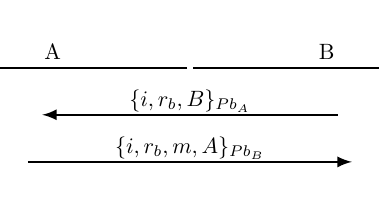
\begin{tikzpicture}[thick,scale=0.8, every node/.style={scale=0.8}]
\matrix (m)[matrix of nodes, column sep=0.5cm,row sep=6mm, nodes={draw=none, anchor=center,text depth=0pt} ]{
A & & B\\[-4mm]
 & $\{i,r_b,B\}_{Pb_A}$& \\[-4mm]
 & $\{i,r_b,m,A\}_{Pb_B}$ & \\[-4mm]
};

\draw[shorten <=-1.5cm,shorten >=-1.5cm] (m-1-1.south east)--(m-1-1.south west);
\draw[shorten <=-1.5cm,shorten >=-1.5cm] (m-1-3.south east)--(m-1-3.south west);
\draw[shorten <=-1cm,shorten >=-1cm,-latex] (m-2-2.south east)--(m-2-2.south west);
\draw[shorten <=-1cm,shorten >=-1cm,-latex] (m-3-2.south west)--(m-3-2.south east);
\end{tikzpicture}
\end{center}
\caption{Shape 3} 
\label{protocol3}
\end{figure}

\begin{Proposition}
Considering assumptions (A1) to (A4), the bundle $\mathcal{B}^{SP}_{pro}(m,i)$ containing two skeleton $st^e_{pro}(m,i)$ and $st^r_{pro}(m,i)$ offers data confidentiality for $m$ and prevents Responder from replaying attack. 
\end{Proposition}

\begin{proof}
\emph{Initator's guarantee}: Firstly, $m$ is extractable in second message by the responder's private key. Moreover, $m$ is secured and integrity by the responder's public key. Assume that $r_b$ uniquely originates in $\mathcal{B}^{SP}_{pro}(m,i)$, initiator can ensure for the unique responder skeleton in $\mathcal{B}^{SP}_{pro}(m,i)$. Finally, the initiator skeleton $st^e_{pro}(m,i)$ holds properties as data confidentiality, data origin authentication and non-replaying attack.

\emph{Responder's guarantee}: Firstly, $m$ is extractable in second message by the responder's private key. Moreover, $m$ is secured and integrity by the responder's public key. When $r_b$ uniquely originates in $\mathcal{B}^{SP}_{pro}(m,i)$, the responder ensures the existence of regular initiator skeleton in $\mathcal{B}^{SP}_{pro}(m,i)$. Finally, the responder skeleton $st^r_{pro}(m,i)$ holds properties as data confidentiality and non-replaying attack.
 \end{proof}

%Model of a private public channel
\subsubsection*{Model of a private channel in original Strand Spaces}\label{private}

Let $\mathcal{B}^{SP}_{pri}(m,i)$ be the shape described at figure~\ref{protocol4} which offers data confidentiality, data origin authentication, and prevents replaying attack, suspending attack and dropping attack.

We simulate non-dropping channel by that whenever attackers drop an out-of-band message, the protocol will be stop at that point. Actually, $\mathcal{B}^{SP}_{pri}(m,i)$ is a variant of $NS$ protocol~\cite{674832} which holds injective agreement and secrecy on $(r_a,r_b)$ between two participants. Injective agreement means that there are unique run of both participants in this protocol. As a result, replaying attacks are clearly avoided. Suspending attack apparently is useless as well. Meanwhile, $m$ in encrypted by $B$'s public key, so $m$ is ensured data confidentiality. 

\begin{figure}
\begin{center}
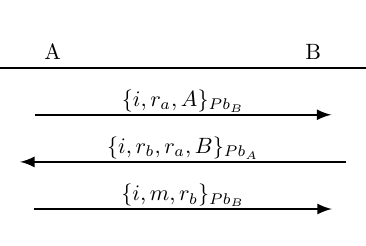
\begin{tikzpicture}[thick,scale=0.8, every node/.style={scale=0.8}]
\matrix (m)[matrix of nodes, column sep=0.4cm,row sep=6mm, nodes={draw=none, anchor=center,text depth=0pt} ]{
A & & B\\[-4mm]
 & $\{i,r_a,A\}_{Pb_B}$ & \\[-4mm]
 & $\{i,r_b,r_a,B\}_{Pb_A}$ & \\[-4mm]
 & $\{i, m,r_b\}_{Pb_B}$ & \\[-4mm]
};

\draw[shorten <=-1.5cm,shorten >=-1.5cm] (m-1-1.south east)--(m-1-1.south west);
\draw[shorten <=-1.5cm,shorten >=-1.5cm] (m-1-3.south east)--(m-1-3.south west);
\draw[shorten <=-1cm,shorten >=-1cm,-latex] (m-2-2.south west)--(m-2-2.south east);
\draw[shorten <=-1cm,shorten >=-1cm,-latex] (m-3-2.south east)--(m-3-2.south west);
\draw[shorten <=-1cm,shorten >=-1cm,-latex] (m-4-2.south west)--(m-4-2.south east);
\end{tikzpicture}
\end{center}
\caption{Protocol 4} 
\label{protocol4}
\end{figure}

\begin{Proposition}
Considering assumptions (A1) to (A4), the shape $\mathcal{B}^{SP}_{pri}(m,i)$ containing two unique skeletons $sk^e_{pri}(m,i)$ and $sk^r_{pri}(m,i)$ offer data origin authentication, data confidentiality for $m$.   
\end{Proposition}

\begin{proof}
The protocol was proved in~\cite{674832} to hold the injective agreement between Initiator and Responder on $r_a$ and $r_b$. Since $m$ is protected under $Pb_B$, attackers cannot overhear $m$. Hence, both skeletons holds properties as data origin authentication and data confidentiality.
\end{proof}

\subsubsection*{Out-of-band Channel Translation}

As can be seen above, four schemes could offers the same security properties as out-of-band channels do. Therefore, they can be used to model a out-of-band channels based protocol in the original Strand Spaces. Let's present how it works. 

Let $st = \langle n_1,...,n_{k-1},n_k,n_{k+1},... \rangle$. We say that if a skeleton $sk$ hooks into a strand $st$ at the node $n_k$ , then $st = \langle n_1,...,n_{k-1},sk,n_{k+1},... \rangle$

\begin{Definition}[OOB Replacement]\label{eos}
The \emph{oob replacement} replaces a message $_o\{m\}$ at node $n=\langle st,j \rangle$ in a strand $st$ by corresponding sending or receiving skeleton that hooks into $st$ at $n$. Precisely, 

\begin{enumerate}
\item [(i)] $+_{lrp}(m)$ and $-_{lrp}(m)$ are replaced by $st^e_{lrp}(m,i)$ and $st^r_{lrp}(m,i)$ respectively;
\item [(ii)] $+_{srp}(m)$ and $-o_{srp}(m)$ are replaced by $st^e_{srp}(m,i)$ and $st^r_{srp}(m,i)$ respectively;
\item [(iii)] $+_{pro}(m)$ and $-_{pro}(m)$ are replaced by $st^e_{pro}(m,i)$ and $st^r_{pro}(m,i)$ respectively;
\item [(vi)] $+_{pri}(m)$ and $-_{pri}(m,i)$ are replaced by $st^e_{pri}(m,i)$ and $st^r_{pri}(m,i)$ respectively;\end{enumerate}
\end{Definition}

\begin{Definition}[OOB Equivalent Strand] Let $st^{ESP}$ be a strand of a protocol modelled in extended Strand Spaces. The strand $st^{SP}$ is called be an \emph{OOB equivalent strand} modelled in original Strand Spaces model for $st^{ESP}$ if $st^{SP}$ is the strand after applying the OOB replacement to all out-of-band messages in $st^{ESP}$.
\end{Definition}

By extension to the bundle, we have an OOB equivalent bundle as follows. 

\begin{Definition}[OOB Equivalent Bundle]\label{iopmf} A bundle $\mathcal{B}^{SP}$ is called an \emph{OOB equivalent bundle} for a bundle $\mathcal{B}^{ESP}$ modelled in extend Strand Spaces if $\mathcal{B}^{SP}$ consists of corresponding OOB equivalent strands of all strands in $\mathcal{B}^{ESP}$. 
\end{Definition}

\subsection{Attack Transformation}\label{attacktransform}

We simulate the suspending event by a storing penetrator strand which receives any message, and reuses it later. 

\begin{Definition}[Storing Penetrator Strand]
$st^s_p$ is a \emph{storing penetrator strand} if 
\begin{itemize}
\item $\forall m \in \mathcal{M}$ in $st^s_p$, then $\exists n \in st^s_p, sign(n) = -, term(n) = m$;
\item $\forall n' \in st^s_p, sign(n') = +,$ then $\exists n \in st^s_p, sign(n)= -, term(n)= term(n')$.
\end{itemize}
\end{Definition}

Let $t_1$, $t_2$, $t_3$ respectively denote terms of first message, second message (if existing) and third message (if existing) in the four shapes defined in previous section. Let $r_b'$ denote a nonce generated by penetrator. Let $st^s_p$ be a storing penetrator strand. $h, h1\in st^s_p$ such that $term(h) = term(t1)$, $term(h1) = term(h)$, and $term(h_2) = term(t_2)$. The table~\ref{attacktrans} depicts attacker's capabilities on each $\mathcal{B}^{SP}_o(m,i)$. The set of these strands is noted as $\mathcal{X}^{SP}$.  

\begin{table}[b]
\centering
\caption{\textsc{Attack Transformation from Extended Strand Spaces to Original Strand Spaces}}
\label{attacktrans}
{\scriptsize
\begin{tabular}{ l l l l l l l }
\hline
\multicolumn{1}{c}{Attack} & \multicolumn{4}{c}{Type of Channel} \\
\hline
\hline
 & Long-range Public & Short-range Public & Protected & Private \\
\hline\hline
$OVH^{SP}$ & $\langle -t1,+t1,+m \rangle$ & $ \langle -t3,+t3,+m \rangle$ & \O & \O \\ \hline
$SUS^{SP}$ & $ \langle -t1, +h \rangle$ & \O & $ \langle -t2,+h \rangle$ & \O \\ \hline
$REL^{SP}$ & $\langle -h, +h1 \rangle$ & \O & $ \langle -h,+h2 \rangle$ & \O \\ \hline
$DRP^{SP}$ & $ \langle -t1 \rangle$ & $ \langle -t1,$ & $\langle -t2 \rangle$ & \O \\
  &  & $+(\{i,r_b',r_a,$ & \\
  &  & $"BtoA"\}_{Pb_A}),$ & \\
  &  & $-t3 \rangle$ & \\ \hline
$REP^{SP}$ & $ \langle -t1, $ & \O & \O & \O \\
 	& $+t1,+t1 \rangle$& & &\\ \hline
\end{tabular}
}
\end{table}

We summarise attack transformation in each type of out-of-band channels in table~\ref{attacktrans}.

A natural question arising is: if there an attack against a transformed protocol in original Strand Spaces is found, is there a corresponding attack on the initial protocol in extended Strand Spaces? This problem is discussed in the subsection~\ref{reverse}. 

\subsection{Proofs}\label{proof}

The proof we will obtain in this paper follows a simple concept to establish the desired results: \emph{A protocol bundle is secure in extended Strand Spaces model if its equivalent OOB bundle is secured}. Or, \emph{whenever there is an attack on extended Strand Spaces model, there is an attack on the equivalent OOB bundle}. Formally presenting, we state this concept into a theorem as follows. 

\begin{Proposition}
Let $\mathcal{B}^{ESP}$ be a normal execution of a protocol $\mathcal{P}$ modeled in the extended Strand Spaces, and $\mathcal{B}^{SP}$ be an OOB equivalent bundle of $\mathcal{B}^{ESP}$. Whenever there is an attack against $\mathcal{B}^{ESP}$, then there is an attack against $\mathcal{B}^{SP}$. 
\end{Proposition}

This proposition is proved by lemmas from~\ref{lemma511} to \ref{lemma514}. 

\begin{Lemma}\label{lemma511}
Let $\mathcal{A}^{ESP}$ be a set of all terms in $\mathcal{B}^{ESP}$, and $\mathcal{A}^{SP}$ be a set of all terms in $\mathcal{B}^{SP}$ . For all $t \in \mathcal{A}^{ESP}$, then $t \in \mathcal{A}^{SP}$. 
\end{Lemma}
\begin{proof}
According to the sub-sections~\ref{OOB-transform}, term $m$ in all of four shapes $\mathcal{B}^{SP}_o(m,i)$ has the same structure and direction as one in $_o(m)$. For instance, message $_{lrp}(m,i)$ from $A$ to $B$ is presented as $(m, \{i,\{h(m)\}_{Pr_a},A\}_{Pb_B})$ in $\mathcal{B}^{SP}_{lrp}(m,i)$. Moreover, defined in the definition~\ref{eos}, the replacement only happens on out-of-band terms. As a consequence, $\forall t \in \mathcal{A}^{ESP}, t \in \mathcal{A}^{SP}$.
\end{proof}

\begin{Lemma}\label{lemma512}
$\mathcal{B}^{SP}$ preserves partial ordering $\lesssim$ in $\mathcal{B}^{ESP}$.    
\end{Lemma}

\begin{proof}
Assume that $n \lesssim n' \in \mathcal{B}^{ESP}$, and $t \sqsubseteq term(n) = +_o(m), t' \sqsubseteq term(n')$,  there exists nodes $n_{sp},n'_{sp} \in \mathcal{B}^{SP}$ so that $t \sqsubset term(n_{sp}), t' \sqsubseteq term(n'_{sp})$, and $n_{sp} \lesssim n'_{sp} $. This is obtained by following facts. 
\begin{itemize}
\item According to lemma~\ref{lemma511}, $\forall t,t' \in \mathcal{A}^{ESP}$, then $t,t' \in \mathcal{A}^{SP}$; and directions of $t$ and $t'$ in $\mathcal{B}^{ESP}$ are preserved $\mathcal{B}^{SP}$.
\item After the replacement, $sk^e_o(m,i)$ is positioned before $n'_{sp}$ in $\mathcal{B}^{SP}$ where term $term(n'_{sp})$ = $term(n')$;
\item $\exists n_{sp} \in sk^e_o(m,i)$ so that $t \sqsubseteq term(n_{sp})$. 
\end{itemize}

As the result of these, $n_{sp} \lesssim n'_{sp}$. Likewise, we have the same proof if $term(n)=-_o(m)$, or $term(n')= _o(m)$.
\end{proof}

\begin{Lemma}\label{sameattack}
Attacker's knowledge and capabilities in $\mathcal{X}^{ESP}$ on $_o(m)$ are similar to ones in $\mathcal{X}^{SP}$ on $\mathcal{B}^{SP}_o(m,i)$. 
\end{Lemma}
\begin{proof}
We are going to give a proof of a long-range public out-of-band channel. The proofs of other channels can be obtained in the same way. Assume that, the message $_{lrp}(m)$ is transmitted over a long-range public channels. Intuitively, attackers can overhear, suspend, release, drop, and replay the message. 

According to the table~\ref{attacktrans}, for the message $(m, \{i,\{h(m)\}_{Pr_a},A\}_{Pb_B})$:
\begin{itemize}
\item $m$ is extracted by $OVH^{SP}$ and $S$;
\item the message is received and held in a storing penetrator strand $st^s_p$ by $SUS^{SP}$;
\item the message is sent from $st^s_p$ by $REL^{SP}$;
\item the message is copied and replayed by $REP^{SP}$;
\item the message is dropped by $DRP^{SP}$
\end{itemize}

The attacker obviously cannot modify the message $(m, \{i,\{h(m)\}_{Pr_a},A\}_{Pb_B})$ since the keys are pre-authenticated. Finally, what the attacker can do with $_{lrp}(m)$ is similar to what he does with $(m, \{i,\{h(m)\}_{Pr_a},A\}_{Pb_B})$.
\end{proof}

\begin{Lemma}\label{lemma514}
If $\mathcal{B'}^{ESP}$ is an execution of $\mathcal{P}$ in which a attacker strand violates goals of $\mathcal{B}^{ESP}$, then $\mathcal{B'}^{SP}$, another shape of $\mathcal{B}^{SP}$, has an attacker strand violates $\mathcal{B}^{SP}$'s goals (similar to $\mathcal{B}^{ESP}$'s).
\end{Lemma}

\begin{proof}
In general, we can assume that the goals of $\mathcal{B}^{ESP}$ are agreement and secrecy on a data set $ds$ between participants $A$ and $B$.  Attackers win the game if $A$ and $B$ receive different $ds$. We assume that $\mathcal{B'}^{ESP}$ contains a attacker strand so that the attacker wins this game. Apparently, $A$ has $ds_A$ while $B$ has $ds_B$, and $ds_A \not= ds_B$. 

Mechanically, $ds_A$ or $ds_B$ are constructed by a sequence of events based on attacker's knowledge about terms, the protocol structure and his capabilities (precisely on Dolev-Yao strands, and $\mathcal{X}^{ESP})$. For example, to produce $\{m,A\}_k$, the attacker uses $OVH$ on $+_o(m)$ from $A$ to $B$ somewhere in the protocol, $SUS$ to suspend the message $+_o(m)$ , $REL$ to release the message, $K$ to generate $k$, and $E$ to produce $\{m,A\}_k$. 

Provided in the lemma~\ref{sameattack}, attacker's capabilities in $\mathcal{X}^{ESP}$ on any term $t \in \mathcal{A}^{ESP}$ are similar ones in $\mathcal{X}^{SP}$ on $t \in \mathcal{A}^{SP}$. For instance, an attacker's sequence in $\mathcal{B'}^{ESP}$ such as ($OVH$, $SUS$, $REL$, $K$, $E$) can be interpreted as ($OVH^{SP}$,$SUS^{SP}$, $REL^{SP}$, $K$, $E$) to produce $\{m,A\}_k$ when $+_o(m)$ is translated into $sk^e_o(m,i)$. 

Therefore, regarding to lemma~\ref{lemma512}, and in the same way the attack constructs $ds_A$ or $ds_B$ in $\mathcal{B'}^{ESP}$, the attacker can produce a sequence of events to construct $ds_A$ or $ds_B$ against goals of $\mathcal{B}^{SP}$. Finally, $\mathcal{B'}^{SP}$ is another execution of $\mathcal{B}^{SP}$ which contains this sequence.
\end{proof}

\subsection{Reversed Attack}\label{reverse}

The problem is when an attack against the transformed protocol is found in $\mathcal{B}^{SP}$, does a corresponding attack exist $\mathcal{B}^{ESP}$? If it is the case, is it possible to figure it out? 

For the long-range public, we easily replace the $\langle -t1, +h \rangle $ by $SUS$ strand, $\langle -t1,+t1,+m \rangle$ by $OVH$ strand, and $ \langle -h,+h1\rangle$ by $REL$ strand, and $ \langle -h_1, +t1,+t1 \rangle$ by $REP$ strand. Then we remove other related messages using the index number $i$, and remove related messages. The protected channels can proceed by the same way. 

However, the case of a short-range public channel is more complicated. We have to search for patterns corresponding to short-range public channel in attack bundle. Whenever we find a negative node having a third message form, we must look for previous nodes using the index $i$. If they exist, then we remove them and replace the third one with $DRP$ strand. Otherwise, if they do not exist, we replace the third message with $OVH$ message, then remove related nodes in attack bundle using the $i$ index, and remove $sk^r_p$.

Eventually, by this manual way, we can reverse an attack on original Strand Spaces into an attack on Strand Spaces. However, we note that if the protocol features messages sent on insecure channels similar to messages obtained when transforming bundles using OOB channels, we cannot conclude. 

\subsection{Example}

In this part, we analyse Wong and Stajano protocol~\cite{10.1109/MPRV.2007.76} using the out-of-band translation. The transformation of the protocol in original Strand Spaces, displayed in~\ref{twong-stajano-protocol}, is formally defined below. 

\begin{figure}[b]
\begin{center}
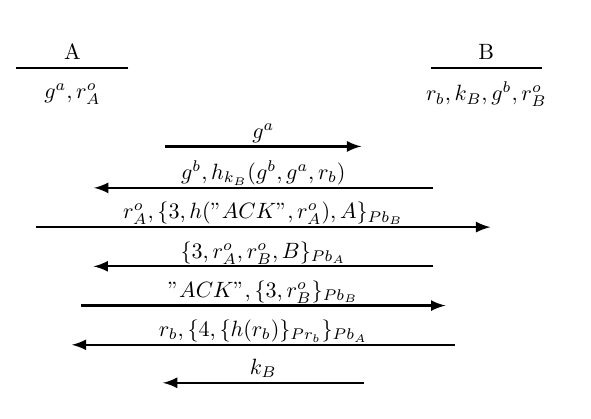
\begin{tikzpicture}[thick,scale=0.8, every node/.style={scale=0.8}]
\matrix (m)[matrix of nodes, column sep=0.1cm,row sep=5mm, nodes={draw=none, anchor=center,text depth=0pt} ]{
A & & B\\[-4mm]
$g^a,r^o_A$ & & $r_b,k_B,g^b,r^o_B$ \\[-4mm]
& $g^a$ & \\[-4mm]
& $g^b, h_{k_B}(g^b,g^a,r_b)$ & \\[-4mm]

 & $r^o_A,\{3, h("ACK",r^o_A),A\}_{Pb_B}$ & \\[-4mm]
 & $\{3,r^o_A,r^o_B,B\}_{Pb_A}$ & \\[-4mm]
 & $"ACK",\{3,r^o_B\}_{Pb_B}$ & \\[-4mm]

 & $r_b, \{4,\{h(r_b)\}_{Pr_b}\}_{Pb_A}$ & \\[-4mm]

& $k_B$ & \\[-4mm]
};

\draw[shorten <=-0.5cm,shorten >=-0.5cm] (m-1-1.south east)--(m-1-1.south west);
\draw[shorten <=-0.5cm,shorten >=-0.5cm] (m-1-3.south east)--(m-1-3.south west);

\draw[shorten <=-1cm,shorten >=-1cm,-latex] (m-3-2.south west)--(m-3-2.south east);
\draw[shorten <=-1cm,shorten >=-1cm,-latex] (m-4-2.south east)--(m-4-2.south west);

\draw[shorten <=-1cm,shorten >=-1cm,-latex] (m-5-2.south west)--(m-5-2.south east);
\draw[shorten <=-1cm,shorten >=-1cm,-latex] (m-6-2.south east)--(m-6-2.south west);
\draw[shorten <=-1cm,shorten >=-1cm,-latex] (m-7-2.south west)--(m-7-2.south east);

\draw[shorten <=-1cm,shorten >=-1cm,-latex] (m-8-2.south east)--(m-8-2.south west);

\draw[shorten <=-1cm,shorten >=-1cm,-latex] (m-9-2.south east)--(m-9-2.south west);
\end{tikzpicture}
\end{center}
\caption{Transformed Wong-Stajano Protocol with Unidirectional Channel} 
\label{twong-stajano-protocol}
\end{figure}



\begin{Definition}
An infiltrated Strand Spaces $(\Sigma,\mathcal{B})$ is a model of Wong-Stajano protocol if $\Sigma$ is the union of the three following kind of strands:
\begin{itemize}
\item \emph{Penetrator strands} $s \in \mathcal{B}$,
\item \emph{Initiator strand} with strand: {\footnotesize $Init[r_b,k_B,g^a,g^b,r^o_A,r^o_A,Pk_A,Pr_a,Pk_B,Pr_b]$}.
\item \emph{Responder strand} with strand: {\footnotesize $Resp[r_b,k_B,g^a,g^b,r^o_A,r^o_B,Pk_A,Pr_a,Pk_B,Pr_b]$}.
\end{itemize}
\end{Definition}

Initiator's guarantee for transformed Wong-Stajano protocol is stated as follows:

\textit{Let $\mathcal{B}$ be a bundle containing a strand $st'$ in \\ {\footnotesize $Init[r_b,k_B,g^a,g^b,r^o_A,r^o_B,Pk_A,Pr_a,Pk_B,Pr_b]$} of height 7. \\ If $r^o_A$ is uniquely originating on $st$, then $\mathcal{B}$ contains a unique strand $st'$ in\\ {\footnotesize $Resp[r_b,k_B,g^a,g^b,r^o_A,r^o_A,Pk_A,Pr_a,Pk_B,Pr_b]$} of height 7. \\ Moreover, both strands agree on $g^a,g^b$.}

\begin{Proposition}
Initiator's guarantee does not hold for transformed Wong Stajano Protocol. 
\end{Proposition}

\begin{proof}
To prove the initiator's guarantee, we must ensure that all of nodes of the responder strand are regular. Let analyse them below.
Since $st$ receives a term \begin{center}$(r_b, \{4,\{h(r_b)\}_{Pr_b}\}_{Pb_A})$\end{center}, we are sure that that a regular node, called $\langle n',6\rangle $, owes this term. This node $\langle n',6\rangle $ belongs to a regular strand $st'$ in $Resp[r_b,k_B,*,g^b,*,r^o_B,Pk_A,Pr_a,Pk_B,Pr_b]$.

Now, let analyse other positive nodes in $st'$ including $\langle st',2\rangle ,\langle st',4\rangle ,\langle st',7\rangle $. Observing that these nodes do not correspond to any authentication tests, they could be on some penetrator strands. 

Looking at node $\langle st',2\rangle $, despite of the origination of $r_b$ in this node, $r_b$ cannot be seen by current initiator strand. Then, when $r_b$ is received in $\langle st,6\rangle$, it could be sent from other previous sections other than the current section. 

As a matter of fact, if an attacker $X$ obtains $r_b$ in a previous Initiator session with a regular responder strand, attackers can reopen a session as a fake responder, and later use $r_b$ to reproduce $term(\langle st',2\rangle )$. Formally saying, the penetrator strand is the following:\begin{center} $\langle-r_b,-k_X,-g^a,-g^{x}, +\{B, g^{x}, h_{k_X}(B,g^{x},g^a,r_b)\}\rangle$\end{center} 
Intuitively, reusing $\{r_b, \{4,\{h(r_b)\}_{Pr_b}\}_{Pb_A}\}$ of previous section, and generating term$(\langle st',4 \rangle)$and term$(\langle st',7 \rangle)$, attackers easily reproduce a fake responder strand $st'$ in order to finish a proper protocol run with current Initiator. 

Finally, initiator's guarantee does not hold.  

\end{proof}

From the counter-example found above for the transformed Wong Stajano protocol, it is possible to rebuild the attack found in~\cite{ttnguyen} against original Wong Stajano protocol by proceeding a reverse analysis as presented in subsection~\ref{reverse}. 

Additionally, when we analyse the transformed Wong Stajano protocol in AVISPA~\cite{Armando:2005:ATA:2153230.2153265}, we get the same result as we did in Strand Spaces model. Through this result, we strongly believe that our implementation can work on other automatic security verification tools. 

\section{Conclusion}

In this chapter, we extended the original Strand Spaces model to be able to analyse secure device pairing protocols. To achieve this, we modified the model so that it becomes possible to take into account protocols using several kind of channels, including OOB channels. The penetrator model has been adapted in consequence. This extension was used to formalise and analyse the Wong-Stajano mutual authentication protocol with unidirectional OOB channel. It successfully pointed us some flaws in the Wong-Stajano protocol that have never been noticed before to our knowledge. 
 
Aforementioned works on this topic, mainly apply existing verification tools initially. We rather chosen to define a dedicated formalism able to model the specificities of device pairing protocols in a natural manner, and the results obtained so far seems  promising. 

In last contribution of this chapter, we gave an interpretation of these properties into cryptographic schemes by defining out-of-band equivalent strand and out-of-band equivalent bundle that describes a protocol modelling in our extended Strand Spaces into original theory. We also presented results that show how protocol's goals and attacks are translated. 

In close future, we continue studying more out-of-band channel-based protocols using our mapping function. We will also analyse them using automatic security verification tools like AVISPA~\cite{Armando:2005:ATA:2153230.2153265}, Casper/FDR~\cite{596779}, and Proverif~\cite{Diaz2014149}. 

%% Chapter Template

\chapter{Secure Neighbour Discovery Protocols} % Main chapter title

\label{Chapter4} % Change X to a consecutive number; for referencing this chapter elsewhere, use \ref{ChapterX}

\lhead{Chapter 4. \emph{Secure Neighbour Discovery Protocols}} % Change X to a consecutive number; this is for the header on each page - perhaps a shortened title

%----------------------------------------------------------------------------------------
%	SECTION 3
%----------------------------------------------------------------------------------------

We have already presented a set of device pairing protocols and formally analysed them at the previous chapters. Basically, by adapting human assistance, wireless devices can establish secure connections among them. Before this stage, each device, indeed, must know existence of its partners. Certainly, ability to determine the existence of participants within physical range in many systems from cellular infrastructure-based networks, wireless local area network to sensor networks, and short range wireless technologies is fundamental problem. Moreover, security mechanisms for it should be seriously considered. 

One potential threat is that due to different wireless interfaces with different signal power, false results from distance calculation in many neighbour discovery mechanisms might appear. The threat is an old-school problem in traditional wireless networks, but it becomes a serious in distributed systems with heterogeneous devices. Attackers can take advantage to generate false connections, that significantly reduces stability of the systems. This has not mentioned before. 

We put ourselves deeply between these problems, and find that some particular neighbour discovery protocols using time-based, or location-based mechanisms are vulnerable. Meanwhile, current formal verification reasoning about security neighbour discovery protocols cannot resolve the problems. This motivates us to study more secure neighbour discovery mechanisms in context of Internet of Things where a huge amount of heterogeneous devices are interoperating. 

Contributions of this chapter are following:
\begin{enumerate}
\item We present existing neighbour discovery protocols, address their limitations, and present some incorrect existing protocols.  
\item We adapt our formalisation on Strand Spaces with some extensions on physical characteristics and some helpful propositions to deal with statuses of links among principals. 
\item Our model allows us obtain a notable result. We prove that time-based or distance-based neighbour discovery schemes cannot confidentially achieve their goals due to difference of physical signal power of principals. 
\end{enumerate}

Chapter 4 begins with a comprehensive survey of current proposals of neighbour discovery techniques, and vulnerabilities. We then present some incorrect protocols and conduct correct ones. We conduct formalisation based on Strand Space in the next part.  
 
 \section{Overview on Neighbour Discovery Protocols}

<<<<<<< HEAD
To begin with, we introduce a definition of a neighbour discovery protocol (NDP) referred at ~\cite{ndp}:
\begin{Definition}
A neighbour discovery protocol is a protocol that operates in link layer of Internet model. It is responsible for auto-configurating nodes, discovery of other nodes on network, determining link-layer addresses of other nodes, and maintaining reachability information about paths to other active neighbour nodes as well. 
\end{Definition}

For instance, in perfect environment with no obstacle and noise, a device can determine its honest neighbours using flying time measurement. A device, called $A$, broadcasts a greeting message to a potential device, called $B$, then $B$ replies to $A$ quickly after receiving this message. Afterward, when completely observing the feed-back message, $A$ measures the time-of-flight, and multiplies it by signal propagation speed in current medium to obtain the distance. If the distance is lower than a pre-defined threshold, $A$ concludes that $B$ is its neighbour.

Above protocol is definitely insecure in environment with existence of attackers. But, it is so important to be fortified. We state the goal of secure neighbour discovery protocol (or SEND) as follows: 

\begin{Definition}[SEND Goal]
Whenever A declares that B is A’s neighbour after A’s SEND process, B apparently runs the protocol and is a desired neighbour of A. Moreover, both sides are closer than their signal ranges.
\end{Definition}

In this session, we explain why neighbour discovery protocols are vital parts in current systems. Then after presenting their threats and vulnerabilities, we sum up existing approaches in categories.
=======
Neighbour discovery is the process by which a node in a network determines the number and identity of other nodes in its vicinity. In wireless context, neighbours are usually defined as nodes that lie within radio range of each other. Nodes considered as neighbours may cooperate in the performance of various tasks such as communications, sensing, and localisation. For instance, in perfect environment with no obstacle and noise, a device can determine its honest neighbours using flying time measurement. A device, called $A$, broadcasts a greeting message to a potential device, called $B$, then $B$ replies to $A$ quickly after receiving this message. Afterward, when completely observing the feed-back message, $A$ measures the time-of-flight, and multiplies it by signal propagation speed in current medium to obtain the distance. If the distance is lower than a pre-defined threshold, $A$ concludes that $B$ is its neighbour.

However, the discovery process is easily abused by malicious ranging activities of attackers in wireless environments. So, there are many approaches for securely discovering neighbours in wireless network. In this session, we explain why neighbour discovery protocols are vital parts in current systems. Then after presenting their threats and vulnerabilities, we sum up existing secure approaches in categories.
>>>>>>> 3d6cc25ad869467a057daa522b35e3cad82b4604

\subsection{Neighbour Discovery Applications}

NDP is discovered under a form of a principal part of many sensitive applications such as physical authentication, network authentication , routing built-up, and localisation. This classification is referred from ~\cite{Marcinthesis}.

\subsubsection*{Physical Authentication}

In some applications, value of distance between two devices is vital to assess authentication goals. For instance, in Passive Keyless Entry and Start~\cite{waraksa1990passive}, a RFID reader can estimate a travelling message flying time to imply distance to companion tags. Similarly to RFID, NFC technology allows smartphones to communicate with other devices such as speakers, headphones or even other smartphones in very short proximity. As the fact of that, neighbour discovery enables devices to find each other. 

\subsubsection*{Network Authentication}
Wireless network demands devices to be authenticated before they access and communicate with others. For instance, when a telephone is willing to access the Internet via a WLAN access point, it must stay in the signal range of the access point. For that purpose, neighbour discovery is a primary part for wireless communications. 

\subsubsection*{Localisation}

When a device wishes to know its current location, it starts broadcasting messages to close GPS satellites, or close WLAN access points to obtain its location information. However, when GPS or WLAN signal is disabled by noise and obstacles due to weather conditions, tree cover, or surrounding buildings, or walls, neighbours' location information could help. For instance, a car cannot locate itself in a long tunnel, then it derives its own location by asking surrounding cars. Hence, these processes apparently stand on a neighbour discovery protocol.

\subsubsection*{Routing Built-up}

Before using a service in ad-hoc network, each device needs to construct a path from itself to a destination. As always, each device constructs a potential network topology by looking for many or all nodes in the network. According to the current network topology, an appropriate path will be picked up. In fact, exploring neighbours is always a primary step at the beginning. 

\subsection{Threat and Vulnerabilities}\label{threatndp}
Classification of threats and vulnerabilities in neighbour discovery protocols is really paintful due to these following reasons. (i) Attackers could be either legitimate principals or outside intruders, or both. (ii) Some attacks happen across layers from physical layer to network one. 

Therefore, we classify the attacks by two ways. The first way is differentiating internal and external attacks. 

\begin{itemize}
\item \textbf{Internal attacks} are types of attacks where intruders compromise several honest participants. Subsequently, they can imitate all honest behaviours, and intentionally generate fake information. 
\item \textbf{External attacks}, in the contrast, are types of attack where intruders are not capable of compromising honest participants and private information. However, they can overhear, reply, and jam messages. 
\end{itemize}

This way sometime makes confusion in some kinds of attacks such as wormhole, and relay attack where attacker could be both insiders and outsiders. As an alternative way, we consider three specific famous attacks on neighbour discovery protocols: \emph{spoofing attack}, \emph{relay attack}, and \emph{tunneling attack}.

\textbf{Spoofing Attack}: In wireless context, spoofing attack is a situation in which an intruder (i) successfully pretends to be someone else to gain a connection to another participant, or (ii) pretends to own a connection to another participant, but actually does not have. The first type is called identification spoofing, while the second is link spoofing attack. 

\textbf{Relay Attack}: According to observation, relay attack demonstrates a situation where messages are relayed between two honest participants by an intruder. Moreover, we consider two types of relay attack. One is store-and-forward relay where a message is completely received before relayed, while others is fast relay where a message is relayed bit-by-bit. 

\textbf{Tunneling Attack} Tunnelling attack, a special kind of replay attack, happens in a long range distance. Two internal adversarial participants tunnel ND messages so that they appear as neighbours on routes constructed by routing protocols. As a result of that, traffic of some nodes on network probably are controlled by these adversarial nodes. In literature, wormhole attack is another name of tunnelling attack. 

There are also two kinds of tunnelling attack in routing context, one is in-band tunnelling, and the other is out-of-band tunnelling. In-band tunnelling describes that messages are encapsulated at one adversarial node, routed through the network as normal packets, and opened at an adversarial companion. In turn of out-of-band tunnelling, messages are routed in a fast private channel.

\subsection{Neighbour Discovery Techniques}

We classify existing notable techniques of neighbour discovery into six primary categories. Additionally, in references to history, neighbour discovery methods assume that all protocol participants are honest, so internal malicious behaviours are not taken into account. Another speaking, traditional approaches only cope with relay attack and wormhole attack. 

\subsubsection*{Time-based Techniques}

There are two main approaches using time-based techniques: single message-scheme and challenge-respond scheme. 

In single message-schemes as ~\cite{Brands:1994aa,Hancke:2005:RDB:1128018.1128472,Capkun:2003:SST:986858.986862,Yih-ChunHu2002}, each device equipped the same synchronized clock periodically broadcasts greeting authenticated messages including its current timestamp. Thank to precisely synchronized clock, any neighbour device receiving this message easily estimates the distance from itself to the source of the message. 

To overcome clock synchronisation limitations, challenge-response schemes such as in~\cite{4110280},\cite{FaridNait-Abdesselam2008} implemented the RTS/CTS mechanism of IEEE 802.11. 

\subsubsection*{Location-based Techniques}

The neighbour information in proposals~\cite{Yih-ChunHu2002,LOUKASLAZOS,LoukasLazos2005, 4146955} is provided at deployment stage, that allows participants to determine their neighbours' location. An alternative method~\cite{1589106} is using secure localisation schemes in which a device includes its location information in its packets. 

<<<<<<< HEAD
However, the assumptions on trusted location information could be impractical. When an adversary compromises one or more honest devices, it can send counterfeit location information to its neighbours. Hence, combination of timestamps and location in ~\cite{Shokri:2009:PSN:1514274.1514302} can offer better security mechanisms.
=======
However, the assumptions on trusted location information could be impractical. When an attacker compromises one or more honest devices, it can send counterfeit location information to its neighbours. Hence, combination of timestamps and location in ~\cite{Shokri:2009:PSN:1514274.1514302} can offer better security mechanisms.
>>>>>>> 3d6cc25ad869467a057daa522b35e3cad82b4604

\subsubsection*{Device Fingerprinting Techniques}

Complicated techniques using RF signal characteristics allow a device to identify other individual devices. The techniques~ \cite{Kasper, OktayUreten2007, VladimirBrik} are based on the fact that every device with a specific wireless adapter and driver differently generates a different signal pattern. By that way, a sensitive receiver probably identifies the source of signal. More complicated techniques ~\cite{SumanJana, 5211943, 819017} used other variables such as frequency error, SYNC correlation, I/Q offset error to enhance identification accuracy. 

\subsubsection*{Channel Fingerprinting Techniques}

Channel states, presented at~\cite{4289438, LiangXiao2008,LiangXiao2009,Liu:2009:SWC:1823633}, characterized by channel impulse response (CIR) in location-specific, or in time-specific can be used to increase accuracy of detecting source of signal. For instance, a device $A$ will not observe correlated CIR from $B$ when $A$ stands outside the $B$'s RF wavelength apart.

\subsubsection*{Directional Antennas-based Techniques}

Multi-directional antennas used in~\cite{Hu04usingdirectional},~\cite{RuiZhang2010} were applied against worm hole attack. Under assumptions of a disk model, each an antenna spans a specific zone and direction. By this characteristic, when a device sends a message in a specific zone, this message is received in opposite zone of another one. 

\subsubsection*{Connectivity-based Techniques}

Connectivity-based techniques basically can detect changes of muti-hops network when any wormhole is created. Moreover, some approaches tried to identify the wormhole and to remove its effects. Two main methods in the literature are centralised schemes and decentralised schemes. 

In the centralised schemes \cite{RuiZhang2010},~\cite{WeichaoWang2007}, visualisation of connectivity graph of the network constructed from coordinates of devices for multi-scaling dimension can be monitored either manually by human operator or automatically by software to detect and localise the wormhole. 

In decentralised schemes, k-hops neighbour information used in~\cite{RiteshMaheshwari}\cite{4699583} were considered as local connectivity to detect and remove a false link in network. Some alternative methods~\cite{RiteshMaheshwari} and ~\cite{5993472} used features generalised edge-clustering coefficient to eliminate connectivity model.

\section{Vulnerabilites of Exisiting Protocols}

This section presents some notable flaws in some famous protocols. The problem in~\cite{Brands:1994aa} was introduced at ~\cite{6234408}, while the other one was found in~\cite{lin2006}. 

\subsection{Brands \& Chaum Protocol Vunerabilities}

Brands \& Chaum(BC) protocol \cite{Brands:1994aa}, the famous distance bounding protocol, enables a verifier to properly estimate the physical distance to its authenticated prover. The protocol works as follows.
\begin{enumerate}
\item Both sides generate their own random number, then rapidly exchanges bit-by-bit to together.
\item The verifier sends a message consisting of the two random numbers, and its signature to the verifier. 
\item The verifier verifies the distance, random values, and the prover's identity in order to accept the connection
\end{enumerate}

To simplify the protocol, we consider the rapid bit-exchange channel as a short-range public out-of-band channel for transmitting random values. The protocol is described below. 

\begin{center}
\begin{flushleft}
 \emph{M1}: $A \rightarrow B :\{A,B\}$ \\
\emph{M2}: $[B \rightarrow A]_o :\{N_B\}$ \\
\emph{M3}: $[A \rightarrow B]_o : \{N_A\}$\\
<<<<<<< HEAD
\emph{M4}: $B \rightarrow A :\{N_A \otimes N_B\}$ \\
=======
\emph{M4}: $B \rightarrow A :\{N_A \oplus N_B\}$ \\
<<<<<<< HEAD
\emph{M5}: $B \rightarrow A : \{|N_A,N_B|\}_{KB}$
=======
>>>>>>> leneutre/master
\emph{M5}: $B \rightarrow A : \{N_A,N_B\}_{KB}$
>>>>>>> 3d6cc25ad869467a057daa522b35e3cad82b4604
\end{flushleft}
\end{center}

To violate the SEND goal, attacker $P$ must make a device $A$ to accept him as the prover. Moreover, the authors did not cover the attack where a distant party with a secret key cooperates with a close party (without conveying secret keys) to complete a protocol. As a result, discovered in the paper~\cite{6234408}, a flaw exploits at the last phase by using an advantage of a high power antenna. The attack scenario is presented at figure~\ref{fig:hijacking_case}. 

\begin{figure}
	  \caption{BC Protocol Attack}\label{fig:hijacking_case}
	  \centering
 		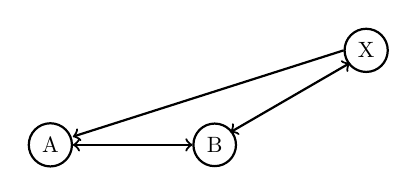
\begin{tikzpicture}[thick,scale=0.8, every node/.style={scale=0.8}]
		\draw [<->](1,1) node[anchor=east,circle,draw]{A} to (2.9,1) node[anchor=west,circle,draw]{B};
		\draw [<-](1,1.13) to (5.3,2.5) node[anchor=west,circle,draw]{X};
		\draw [<->](3.5,1.2) to (5.4,2.3);
	    \end{tikzpicture}
		
		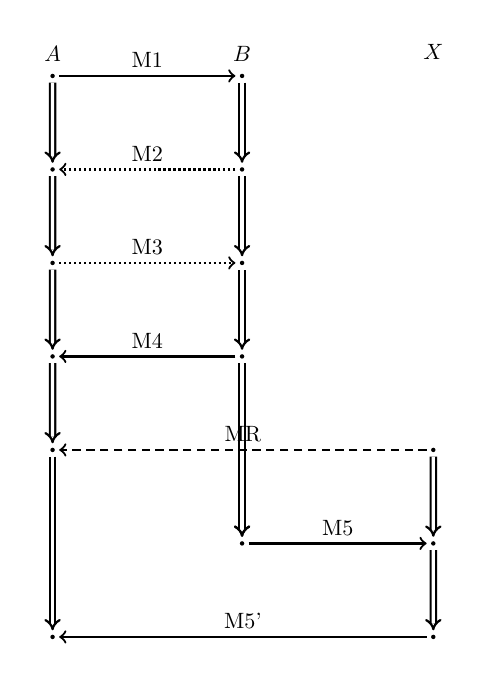
\begin{tikzpicture}[implies/.style={double,double equal sign distance,-implies},
  			 dot/.style={shape=circle,fill=black,minimum size=2pt,
             inner sep=0pt,outer sep=2pt},thick,scale=0.8, every node/.style={scale=0.8}]
		\matrix[matrix of nodes] {
  		|[dot,label=above:$A$] (A1)| {} & [2cm] |[dot,label=above:$B$] (B1)| {} & [2cm]|[label=above:$X$] (X1)| {}\\[1cm]
  		 |[dot] (A2)| {} & [2cm] |[dot] (B2)| {} & [2cm]|[] (X2)| {}\\[1cm]
	     |[dot] (A3)| {} & [2cm] |[dot] (B3)| {} & [2cm]|[] (X3)| {}\\[1cm]
		|[dot] (A4)| {} & [2cm] |[dot] (B4)| {} & [2cm]|[] (X4)| {}\\[1cm]
  		 |[dot] (A5)| {} & [2cm] |[] (B5)| {} & [2cm]|[dot] (X5)| {}\\[1cm]
 		 |[] (A6)| {} & [2cm] |[dot] (B6)| {} & [2cm]|[dot] (X6)| {}\\[1cm]
 		 |[dot] (A7)| {} & [2cm] |[] (B7)| {} & [2cm]|[dot] (X7)| {}\\[1cm] };
	
		\draw (A1) edge[->] node[above] {M1} (B1)
	      edge[implies] (A2); 
		\draw [-latex,densely dotted](B2) edge[->] node[above] {M2} (A2);
	     \draw (A2) edge[implies] (A3);
		\draw [-latex,densely dotted](A3) edge[->] node[above] {M3} (B3);
    	  \draw (B1) edge[implies] (B2);
		\draw (B4) edge[->] node[above] {M4} (A4)
    	  edge[implies,implies-] (B3);
		\draw (B2) edge[implies] (B3);
		\draw (A3) edge[implies] (A4);
		\draw (A4) edge[implies] (A5);
		\draw (B4) edge[implies] (B6);
		\draw [-latex,densely dashed](X5) edge[->] node[above] {MR} (A5);
		\draw (B6) edge[->] node[above] {M5} (X6);
		\draw (X5) edge[implies] (X6);
		\draw (X7) edge[->] node[above] {M5'} (A7);
		\draw (B5) edge[implies] (B6);
		\draw (X6) edge[implies] (X7);
		\draw (A5) edge[implies] (A7);
		\end{tikzpicture} 

\end{figure}

\subsection{ADVSIG Vulnerability}

<<<<<<< HEAD
ADVSIG proposed by INRIA group~\cite{Raffo:2004:ASS:1029102.1029106} is a kind of secure routing protocol fortifying for OLSR \cite{Clausen:2003:OLS:RFC3626}. In this protocol, a node wishes to detect neighbour nodes with a direct and bi-directional link. Any link must be checked to be considered validation. We realise that compared to OLSR specification, third message of ADVSIG changed SYMMETRIC LINK status to ASYMMETRIC LINK status. This change may affect to neighbours of A if no new message from A informs that A owns a symmetrical link A to B. The protocol is presented as below. 
\begin{flushleft}
 \emph{M1:} $A \to [B]: \{|\O, \O, t_0|\}_{KA}$\\
 \emph{M2:} $B \to [A]: \{|\{|"A:ASYM\_LINK", t_1|\}_{KB}, \O,t_1|\}_{KB}$\\
\emph{M3:} $A \to [B]: \{|\{|"B:ASYM\_LINK",t_2|\}_{KA},\O ,t_2 |\}_{KA})$\\
 \emph{M4:} $B \to [A] : \{|\{|"A:SYM\_LINK", t_3|\}_{KB} ,\{|"B:ASYM\_LINK",t_2|\}_{KA} ,t_3|\}_{KB})$
=======
ADVSIG proposed by INRIA group~\cite{Raffo:2004:ASS:1029102.1029106} is a kind of secure routing protocol fortifying for OLSR \cite{Clausen:2003:OLS:RFC3626}. In this protocol, a node wishes to detect neighbour nodes with a direct and bi-directional link. Any link must be checked to be considered validation. We realise that compared to OLSR specification, third message of ADVSIG changed SYMMETRIC LINK status to ASYMMETRIC LINK status. This change may affect to neighbours of A if no new message from A informs that A owns a bidirectional link A to B. The protocol is presented as below. 
\begin{flushleft}
 \emph{M1:} $A \to [B]: \{\O, \O, \tau_0\}_{KA}$\\
 \emph{M2:} $B \to [A]: \{\{"A:ASYM\_LINK", \tau_1\}_{KB}, \O,\tau_1\}_{KB}$\\
\emph{M3:} $A \to [B]: \{\{"B:ASYM\_LINK",\tau_2\}_{KA},\O ,\tau_2 \}_{KA})$\\
 \emph{M4:} $B \to [A] : \{\{"A:SYM\_LINK", \tau_3\}_{KB} ,\{"B:ASYM\_LINK",\tau_2\}_{KA} ,\tau_3|\}_{KB})$
>>>>>>> 3d6cc25ad869467a057daa522b35e3cad82b4604
\end{flushleft}

Moreover, every valid link state must satisfy a maximum interval $\delta_{max}$ defined by $|T_{Sender} - T_e | < \delta_{max}$ where $T_{Sender}$ is the value clock of the sender, and $T_e$ is the value clock of receiver. 

<<<<<<< HEAD
Provided that the third message does not include the proof from the second one, Responder cannot ensure if Initiator has been received the second message or not. As the result of that, internal attackers can produce the first and third messages to valid a protocol run with Responder. Additionally,  neighbours of Responder could be impacted by this attack due to two-hop sensing mechanism in the OLSR protocol.  Figure~\ref{advsigattack3} outlines an attacking scenario to ADVSIG where there only appears an asymmetric link X $\rightarrow$ B.
=======
Provided that the third message does not include the proof from the second one, Responder cannot ensure if Initiator has been received the second message or not. As the result of that, internal attackers can produce the first and third messages to valid a protocol run with Responder. Additionally,  neighbours of Responder could be impacted by this attack due to two-hop sensing mechanism in the OLSR protocol.  Figure~\ref{advsigattack3} outlines an attacking scenario to ADVSIG where there only appears an unidirectional link X $\rightarrow$ B.
>>>>>>> 3d6cc25ad869467a057daa522b35e3cad82b4604

\begin{figure}
		\caption{ADVSIG Attack }\label{advsigattack3}
        \centering
        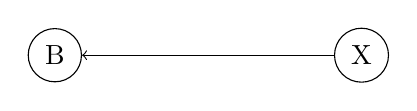
\begin{tikzpicture}
		\draw [<-](1,1) node[anchor=east,circle,draw]{B} to (4.2,1) node[anchor=west,circle,draw]{X};
		\end{tikzpicture}

	    \centering
        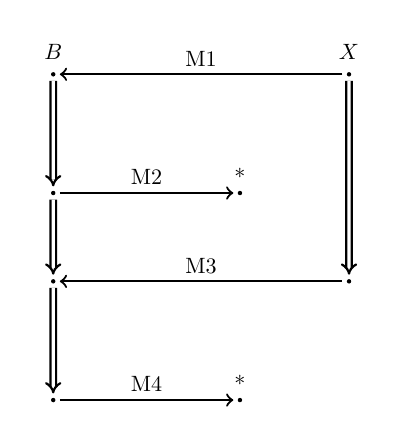
\begin{tikzpicture}[implies/.style={double,double equal sign distance,-implies},
  			dot/.style={shape=circle,fill=black,minimum size=2pt,
  		      inner sep=0pt,outer sep=2pt},thick,scale=0.8, every node/.style={scale=0.8}]
		\matrix[matrix of nodes] {
		  |[dot,label=above:$B$] (B1)| {} & [2cm]|[] (C1)| {}&[1cm] |[dot,label=above:$X$] (X1)| {}\\[1cm]
  		  |[dot] (B2)| {} & [2cm]|[dot,label=above:$*$] (C2)| {}& [1cm]|[dot] (X2)| {}\\[1cm]
  	      |[dot] (B3)| {} & [2cm]|[] (C3)| {}& [2cm]|[dot] (X3)| {}\\[1cm]
 		  |[dot] (B4)| {} & [2cm]|[dot,label=above:$*$] (C4)| {}& [1cm]|[] (X4)| {}\\
		};
		\draw (X1) edge[->] node[above] {M1} (B1)
	      edge[implies] (X3); 
		\draw (B2) edge[->] node[above] {M2} (C2)
	      edge[implies,implies-] (B1);
		\draw (B3) edge[<-] node[above] {M3} (X3)
    	  edge[implies,implies-] (B2);
		\draw (B4) edge[->] node[above] {M4} (C4)
    	  edge[implies,implies-] (B3);
		\end{tikzpicture}

\end{figure}

We found the same problem in the work~\cite{Adnane20131159}. Authors proposed a trusted-based security for OLSR protocols where all participants must trust together. However, internal attackers can successfully create a fake bidirectional link to a target as they do in ADVSIG. 

\subsection{Correctness of ADVSIG}
In this part, we would like to propose a simple correctness of ADVSIG scheme. We attach link proofs for the second and the third message. Thus, the first link proof in the second message is a hash of the first message encrypted by B's public key, while the second link proof in the third message is the link state of the previous one. 

<<<<<<< HEAD
$A$'s signature wrapped by hash function is impossible to be reproduced by any adversary. As the result of that, even the adversary incidentally receives the message of $B$, he cannot create a correct reply. An important note that, after the third message, $A$ fully indicates $B$ be its neighbour. For that reason, physical link guaranty must be done before this step. The scheme is presented as follows. 

\begin{flushleft}
 \emph{M1:} $A \to [B]: \{|\O, \O, t_0|\}_{KA}$\\
 \emph{M2:} $B \to [A]: \{|\{|"A:ASYM\_LINK", t_1|\}_{KB},$ $h(\{|\{|\O, \O, t_0|\}_{KA}|\}pub(B)),t_1|\}_{KB}$\\
\emph{M3:} $A \to [B]: \{|\{| "B:SYM\_LINK",t_2|\}_{KA},$ $\{|"A:ASYM\_LINK", t_1|\}_{KB},t_2 |\}_{KA}$\\
 \emph{M4:} $B \to [A] : \{|\{| "A:SYM\_LINK", t_3|\}_{KB},$ $\{| "B:SYM\_LINK",t_2|\}_{KA} ,t_3|\}_{KB}$
=======
$A$'s signature wrapped by hash function is impossible to be reproduced by any attacker. As the result of that, even the attacker incidentally receives the message of $B$, he cannot create a correct reply. An important note that, after the third message, $A$ fully indicates $B$ be its neighbour. For that reason, physical link guaranty must be done before this step. The scheme is presented as follows. 

\begin{flushleft}
 \emph{M1:} $A \to [B]: \{\O, \O, \tau_0|\}_{KA}$\\
 \emph{M2:} $B \to [A]: \{\{"A:ASYM\_LINK", \tau_1\}_{KB},$ $h(\{\{\O, \O, \tau_0\}_{KA}\}pub(B)),\tau_1\}_{KB}$\\
\emph{M3:} $A \to [B]: \{\{ "B:SYM\_LINK",\tau_2\}_{KA},$ $\{"A:ASYM\_LINK", \tau_1\}_{KB},\tau_2\}_{KA}$\\
 \emph{M4:} $B \to [A] : \{\{ "A:SYM\_LINK", \tau_3\}_{KB},$ $\{"B:SYM\_LINK",\tau_2\}_{KA} ,\tau_3\}_{KB}$
>>>>>>> 3d6cc25ad869467a057daa522b35e3cad82b4604
\end{flushleft}

Now, by proofs, A and B easily verify physical bidirectional links between them. 

\section{Formal Analysis of Neighbour Discovery Protocol}

%The problems in some neighbour discovery protocols introduced in previous section question why they had not discovered when the protocols were being constructed and tested. An expensive answer we say is that they have not exhaustedly analysed in formal methods. Additionally, current formal models are not ready for this problem due to strong assumptions on characteristic of physical wireless interfaces, and attackers' capabilities.   

%To tackle this problem, we construct our formalisation based on Strand Spaces theory. In our formalisation, each event is facilitated with timestamps, location information and signal power, so this allows us to formalise neighbour discovery protocols and to discover the problems we presented in the Introduction section. To begin with, we recap existing models and spot their limitations. 

Due to lack of place, we do not recall here the whole theory of Strand Spaces, but focus on the extensions necessary to examine secure neighbour discovery protocol. For a complete background on Strand Spaces the reader can consult~\cite{674832},~\cite{Guttman:2002:ATS:568264.568267}. The extensions mainly concern the physical notations and the penetrator model...
 
Before presenting our model extensions of Strand Spaces, we formulate some supplementary assumptions concerning physical characteristics of wireless interfaces and environment, that we will have to take into account. 

\subsection{Related Work}

Most current approaches formalised time as timestamps to determine key-expiration \cite{Li:2007:ESS:1338438.1338469} , and integrity of messages via round trip time-of-flight ~\cite{Poturalski:2008:TPS:1456396.1456400, RaphaelJamet}. Meanwhile, location information was considered in problems of correctness of routing protocols~\cite{5230621,Basin:2009:LGP:1616077.1616079}, or evaluating distance between two neighbours in \cite{Poturalski:2008:TPS:1456396.1456400}. Barely found in literature, signal characteristic is an interesting feature mentioned in \cite{Poturalski:2008:TPS:1456396.1456400}. However, this feature is not truly helpful to reveal attacking location and direction. 

Close to our approach, the models~\cite{Yang03modelingvulnerabilities, 4481351} extended Strand Spaces to pick up vulnerabilities in ad-hoc routing protocols while other approaches \cite{Li:2007:ESS:1338438.1338469, Sharp:2007:TTS:2391910.2391948} expressed temporal phenomena, and notably key-expiration. In addition to, metric strand proposed in \cite{Thayer:2010aa} was presented to deal with locale authentication. Nevertheless, no specified attack and proof was provided in this work. 

\subsection{Assumptions}

We explicitly declare some reasonable assumptions as follows:
\begin{itemize}
\item Every participant is equipped with: (I) \textit{various types of wireless devices with different signal powers}, (ii) \textit{precise clock devices}. To make simplicity, radiation power is assumed to stay the same during protocol execution.
\item An \textit{idealized communication environment} is regarded where wireless signal travels on non-obstacle path with speed of light \emph{c}. Following this assumption, when a participant stands on signal propagation region of others, he can listen to their exchanged messages. 
\item A \textit{secure key distribution function} is enabled on all participants. 
\end{itemize}

Furthermore, our current work only focuses on \textit{a static wireless network model} where objects do not change their position due to complexity of modelling dynamic networks. Dynamic network, hence, could be extended and considered in our future work. 

\subsection{Wireless Strand Spaces}

<<<<<<< HEAD
Actually, original Strand Spaces was designed for cryptographic protocols, so it apparently cannot deal with neighbour discovery protocols. To tackle this limitation, we facilitate Strand Spaces model with our extensions to account for wireless context, then we call the \textit{wireless Strand Spaces}. In particular, a node in our model is equipped with \textit{location, timestamp, signal range} values. Location shows where the node is standing, timestamp indicates when a node happens, and signal range refers to how far the wireless signal of the node can reach. As consequence, the definition of a wireless node is presented as belows.

\begin{Definition}[Wireless Node] A \emph{wireless node} $n$ is a tuple of $(t, l_n, t_n, R_n)$ where $t$ is a signed term, $l_n$ is location, $t_n$ is a timestamp, and $R_n$ is signal range.\end{Definition}

Note that, $l_n$, \textit{location of a node n}, is extensible to any Euclidean space. \textit{Distance between nodes} $n$ and $n'$ is noted $dist(l_n,l_n')$ or $dist(n,n')$. \textit{Timestamp}, $t_n$, appears in a node to check freshness property, and it is a value of local clock when an event begins. \textit{Signal range of a node n}, $R_n$, is a positive real number. 
=======

Obviously, original Strand Spaces was designed for cryptographic protocols, so it apparently cannot deal with neighbour discovery protocols. To tackle this limitation, we facilitate Strand Spaces model with our extensions to account for wireless context, then we call the \textit{wireless Strand Spaces}. In particular, a node in our model is equipped with \textit{location, timestamp, signal range} values. Location shows where the node is standing, timestamp indicates when a node happens, and signal range refers to how far the wireless signal of the node can reach. As consequence, the definition of a wireless node is presented as below.

\begin{Definition}[Wireless Node] A \emph{wireless node} $n$ is a tuple of $(t, l_n, \tau_{n}, R_n)$ where $t$ is a signed term, $l_n$ is location, $\tau_{n}$ is a timestamp, and $R_n$ is signal range.\end{Definition}

Note that, $l_n$, \textit{location of a node n}, is extensible to any Euclidean space. \textit{Distance between nodes} $n$ and $n'$ is noted as $dist(n,n')$. \textit{Timestamp}, $\tau_{n}$, appears in a node to check freshness property, and it is a value of local clock when an event begins. \textit{Signal range of a node n}, $R_n$, is a positive real number. According to assumption~\ref{assum}, signal power does not change during a protocol execution; hence, we denote $R_{st}$ is physical signal  propagation of strand $st$. 
>>>>>>> 3d6cc25ad869467a057daa522b35e3cad82b4604

In realistic scenarios, there always exists a gap between two events, so a fixed value $\delta_{tp}$ is noted as a \textit{processing delay} of edge $ (+n) \Rightarrow (-n')$. We continue describing definitions of wireless strand, and wireless bundle. 

\begin{Definition}[Wireless Strand] A \emph{wireless strand} is a strand with wireless nodes.
\end{Definition}

<<<<<<< HEAD
Recall that static network is being discussed in this article; hence, a strand with fixed location is so-called \textit{a fixed wireless strand}. Thus, all nodes in a fixed strand share the same location. To avoid ambitious notions, notion of strand in this section is now refer to a wireless strand. 

In our extension, we need to explicitly distinguish between different types of links. A link is a generic term denoted a relationship between two participants. There are two kinds of links: \emph{logical} and \emph{physical}. While a logical link describes existence of path of a term from one strand to another, a physical one describes a directional and physical path without any relaying point from one strand to another one. Moreover, each type of link has two states: \emph{single} and \emph{double}. A single link means an unidirectional connection when a double link means a bidirectional one. 

Actually, existence of a physical link is usually hard to be correctly criticised due to environment complexity. Hence, in this work, a physical link is simply evaluated by a distance value among participants. Precisely speaking, by any mean, a double physical link exists between two participants if and only if the distance between them is lower than their own signal coverage. Thus, we formally define notations of links as follows.

\begin{Definition}
\begin{itemize}
\item \emph{Single physical link}: $\forall st,st' \in \mathcal{B}$, $plink(st,st', \rightarrow) \Leftrightarrow$ $dist(st,st') \le R_{st}$.
\item \emph{Double physical link}: $\forall st,st' \in \mathcal{B}$, $plink(st,st', \leftrightarrow) \Leftrightarrow$ $(dist(st,st') \le R_{st}) \wedge (dist(st',st) \le R_{st'})$.
\item \emph{Single logical link}: $\forall st, st' \in \mathcal{B}, n \in st, n' \in st', \exists (n_1 \rightarrow^* n_2) \Leftrightarrow \exists link(st, st',\rightarrow)$.
\item \emph{Double logical link}: $\forall st, st' \in \mathcal{B},$ $ \exists link(st, st',\rightarrow) \wedge \exists link(st', st,\rightarrow) \Leftrightarrow \exists link(st, st',\leftrightarrow)$.
=======
Recall that static network is being discussed in this article; hence, a strand with fixed location is so-called \textit{a fixed wireless strand}. Thus, all nodes in a fixed strand share the same location. We denote $loc(st)$ be the location of strand $st$, and $dist(st,st')$ be the distance between two strand $st$ and $st'$. To avoid ambitious notions, notion of strand in this section is now refer to a wireless strand. 

In our extension, we need to explicitly distinguish between different types of links. A link is a generic term denoted a relationship between two participants. There are two kinds of links: \emph{logical} and \emph{physical}. While a logical link describes existence of path of a term from one strand to another, a physical one describes a directional and physical path without any relaying point from one strand to another one. Moreover, each type of link has two states: \emph{unidirectional} and \emph{bidirectional}. 

Existence of a physical link is usually hard to be precisely criticised due to environment complexity. Hence, in this work, a physical link is simply evaluated by a distance value among participants. Another speaking, by any mean, a bidirectional physical link exists between two participants if and only if the distance between them is lower than their own signal coverage. We formally define notations of links as follows.

\begin{Definition}
\begin{itemize}
\item \emph{Unidirectional physical link}: $\forall st,st' \in \mathcal{B}$, $plink(st,st', \rightharpoonup) \Leftrightarrow$ $dist(st,st') \le R_{st}$.
\item \emph{Bidirectional physical link}: $\forall st,st' \in \mathcal{B}$, $plink(st,st', \rightleftharpoons) \Leftrightarrow$ $(dist(st,st') \le R_{st}) \wedge (dist(st',st) \le R_{st'})$.
\item \emph{Unidirectional logical link}: $\forall st, st' \in \mathcal{B}, n \in st, n' \in st', \exists (n_1 \rightarrow^* n_2) \Leftrightarrow \exists link(st, st',\rightharpoonup)$.
\item \emph{Bidirectional logical link}: $\forall st, st' \in \mathcal{B},$ $ \exists link(st, st',\rightharpoonup) \wedge \exists link(st', st,\rightharpoonup) \Leftrightarrow \exists link(st, st',\rightleftharpoons)$.
>>>>>>> 3d6cc25ad869467a057daa522b35e3cad82b4604
\end{itemize}	
\end{Definition}

\subsection{Extended Penetrator Model}\label{penndp2}

<<<<<<< HEAD
Relaying attack and link spoofing attack are two serious malicious events against neighbour discovery goals. \textbf{Spoofing attack} is a situation in which an intruder (i) successfully pretends to be someone else to gain a connection to another participant, or (ii) pretends to own a connection to another participant, but actually does not have. According to observation, \textbf{relay attack} demonstrates a situation where messages are relayed between two honest participants by an intruder. 

These attacks are apparently conducted from a sequence of atomic events such as sending events with high a power antenna  and single replaying events respectively. Hence, we encode the atomic malicious actions into two new penetrator strands. Precisely, given penetrator strand $s_p$, and $n, n' \in s_p$. 
\begin{itemize}
\item[SR.] \emph{Single relay:} \\ $\langle -(t, l_n, t_n, R_n), +(t, l_n', t_{n'}, R_{n'}) \rangle >$ where $t_{n'} - t_n = 0$.
\item [BS.] \emph{Boosting signal:} $\langle +(t, l_n, t_n, R_M) \rangle$ where $R_M$ could be an unlimited value. 
\end{itemize}

At present, single relaying attack is possibly detected by advanced protection mechanisms presented in the previous section. Therefore, we consider the \emph{weak penetrator model} be a model which does not deal with relaying attack. In contrast, \emph{strong penetrator model} has full attacker's capabilities. 

\subsection{Modeling Goals}

We express this goal in Strand Spaces model as an authentication goal:

\emph{Secure Neighbour Disovery Goal:} \textit{For all bundles $\mathcal{B}$, two roles $R, R' \in \mathcal{B}$, and all strand $st$, there exists a strand $st$' such that if $st \in R$ has $ \mathcal{B}_{height}$ i and some protocol assumptions hold then $st' \in R'$ has $\mathcal{B}_{height}$ j and there exists a physical link $plink(st,st',\leftrightarrow)$.}
=======
Along with Dolev-Yao penetrator model~\cite{dolev-yao}, this article considers two physical attacks: relaying attack and link spoofing attack since they are two serious malicious events against neighbour discovery goals. \textbf{Spoofing attack} is a situation in which an intruder (i) successfully pretends to be someone else to gain a connection to another participant, or (ii) pretends to own a connection to another participant, but actually does not have. According to observation, \textbf{relay attack} demonstrates a situation where messages are relayed between two honest participants by an intruder. 

These attacks are apparently conducted from a sequence of atomic events such as sending events with high a power antenna  and single replaying events respectively. Hence, we encode the atomic malicious actions into two new penetrator strands. Precisely, given penetrator strand $s_p$, and $n, n' \in s_p$. 
\begin{itemize}
\item[SR.] \emph{Single relay:} \\ $\langle -(t, l_n, \tau_{n}, R_n), +(t, l_n', \tau_{n'}, R_{n'}) \rangle >$ where $\tau_{n'} - \tau_{n} = 0$.
\item [BS.] \emph{Boosting signal:} $\langle +(t, l_n, \tau_{n}, R_M) \rangle$ where $R_M$ could be an unlimited value. 
\end{itemize}

At present, single relaying attack is possibly detected by advanced protection mechanisms presented in the previous section. Therefore, we consider the \emph{weak penetrator model} be a model which does not deal with relaying attack. In contrast, \emph{strong penetrator model} has full attacker's capabilities. 
We express this goal in Strand Spaces model as an authentication goal:

\emph{Secure Neighbour Disovery Goal:} \textit{For all bundles $\mathcal{B}$, two roles $R, R' \in \mathcal{B}$, and all strand $st$, there exists a strand $st$' such that if $st \in R$ has $ \mathcal{B}_{height}$ i and some protocol assumptions hold then $st' \in R'$ has $\mathcal{B}_{height}$ j and there exists a physical link $plink(st,st',\rightleftharpoons)$.}
>>>>>>> 3d6cc25ad869467a057daa522b35e3cad82b4604

Guttman stated that analysing authentication properties of a protocol means finding right choices for $R$ and $R'$ for $i$, and $j$, and necessary origination assumptions. However, this proving way could extremely cost time and effort when solving a complicated protocol. So, to ease this job, Guttman introduced authentication tests~\cite{authenticationtests} as supporting tools. Following to this idea, we construct our authentication link tests to guarantee whether a protocol satisfies the goal or not.  At first, we introduce a link test edge, and an authentication logical link test. Then, we conduct authentication physical link tests based on time and location estimation. 

\subsection{Logical Link Tests}

<<<<<<< HEAD
To get rid of link spoofing attack, a protocol should support a mechanism to enable a participant to verify whether his protocol-mate has already seen its messages or not. As a solution, challenge-respond mechanisms, described formally as authentication tests, could be used in which a participant delivers a random as a challenge and receives an answer only produced by an intended sender. The answer usually contains a cryptographic part as a proof that allows the participant verifies origin, integrity, or confidentiality of this message. 

One possible particular proof, called \textit{hidden proof}, is a nonce encrypted by pre-shared key, or a nonce encrypted by public key of Initiator, or a hash of nonce and name of Responder. Another one, called \textit{clear proof}, is a part of previous Initiator's message that contains Responder's ID and a timestamp, and is signed by private key of the Initiator. We define notations of \emph{identification factor}, and a \emph{provable component} to express these such proofs. 

\begin{Definition} \emph{An identification factor} in a component $\{|h|\}_K$ is:
\begin{itemize}
	\item(clear-form) \emph{responder's $ID_{Res}$ and a timestamp t} such that $(ID_{Res} \sqsubseteq \{|h|\}_K ) \wedge (t \sqsubseteq \{|h|\}_K$ in which $K$ is a private key of the initiator, or a signature $sig(K)$ encrypted with a private key of the initiator $K$. Or, 
	\item(hidden-form) \emph{a nonce N} such that N $\sqsubseteq \{|h|\}_K$ in which $K$ is a pre-shared secret key or public key of the responder.\end{itemize}
=======
To get rid of link spoofing attack, a protocol should support a mechanism enabling a participant to verify whether his protocol-mate has already seen its messages or not. As a solution, challenge-respond mechanisms, described formally as authentication tests, could be used in which a participant delivers a random as a challenge and receives an answer only produced by an intended sender. The answer usually contains a cryptographic part as a proof that allows the participant verifies origin, integrity, or confidentiality of this message. 

One possible particular proof, called \textit{hidden proof}, is a nonce encrypted by pre-shared key, or a nonce encrypted by public key of Initiator, or a hash of nonce and name of Responder. Another one, called \textit{clear proof}, is a part of previous Initiator's message that contains Responder's ID and a timestamp, and is signed by private key of the Initiator. We define notations of \emph{identification factor}, and a \emph{provable component} to express these such proofs. 

\begin{Definition} \emph{An identification factor} in a component $\{h\}_K$ is:
\begin{itemize}
	\item(clear-form) \emph{responder's $ID_{Res}$ and a timestamp t} such that $(ID_{Res} \sqsubseteq \{h\}_K ) \wedge (t \sqsubseteq \{h\}_K$ in which $K$ is a private key of the initiator. Or, 
	\item(hidden-form) \emph{a nonce N} such that N $\sqsubseteq \{h\}_K$ in which $K$ is a pre-shared secret key or public key of the responder.\end{itemize}
>>>>>>> 3d6cc25ad869467a057daa522b35e3cad82b4604
\end{Definition}

\begin{Definition}\emph{A provable component} is a component which has one of forms:
\begin{itemize}
<<<<<<< HEAD
	\item (clear-form):$\{|m|\}_{Pr(Res)}$ in which $idf \sqsubseteq \{|h|\}_{Pb(Init)} \sqsubseteq m$ where $Pr(Res)$ is a private key of Responder, and $Pb(Init)$ is the public key of Initiator;  
	\item (hidden-from):$\{|m|\}_K$ or $\{hash(m)\}_{Pr(Res)}$ in which $idf \sqsubseteq m$, and K is a pre-shared key, and $Pr(Res)$ is a public key of Responder;
=======
	\item (clear-form):$\{m\}_{Pr(Res)}$ in which $idf \sqsubseteq \{h\}_{Pb(Init)} \sqsubseteq m$ where $Pr(Res)$ is a private key of Responder, and $Pb(Init)$ is the public key of Initiator;  
	\item (hidden-from):$\{m\}_K$ or $\{hash(m)\}_{Pr(Res)}$ in which $idf \sqsubseteq m$, and K is a pre-shared key, and $Pr(Res)$ is a public key of Responder;
>>>>>>> 3d6cc25ad869467a057daa522b35e3cad82b4604
\end{itemize}
\end{Definition}

We conduct \emph{a logical link test}, and \emph{an authentication logical link test} which allows a participant to ensure that none of it's partners completes a protocol run without receiving its messages. We would like to revise the definition of \emph{a test} defined in~\cite{authenticationtests}. 

\begin{Definition}[A Test] 
<<<<<<< HEAD
$t = \{|m|\}_K$ is \emph{a test} for $a$ in $n$ if:
=======
$t = \{m\}_K$ is \emph{a test} for $a$ in $n$ if:
>>>>>>> 3d6cc25ad869467a057daa522b35e3cad82b4604
\begin{enumerate}
\item $a\sqsubseteq t$ and $t$ is a component of $n$;
\item The term $t$ is not a proper subterm of a component of any regular node $n' \in \Sigma$. 
\end{enumerate}
The edge $n \Rightarrow^+ n'$ is \emph{a test} for $a$ if $a$ uniquely originates at $n$ and $n \Rightarrow^+ n'$ is a transformed edge for $a$. 
\end{Definition}

<<<<<<< HEAD
\begin{Definition}[Logical Link Test] The edge $n \Rightarrow^+ n'$ is a \emph{logical link test} for an identification factor $idf$ in $t = \{|m|\}_K \sqsubseteq term(n')$ if it is a test for $idf$ in which $K \not\in P$ and $t$ is a provable component for $idf$ in $n'$
\end{Definition}

The authentication logical link test below results a double logical link between two strands $st$ and $st'$ in a bundle. 
=======
\begin{Definition}[Logical Link Test] The edge $n \Rightarrow^+ n'$ is a \emph{logical link test} for an identification factor $idf$ in $t = \{m\}_K \sqsubseteq term(n')$ if it is a test for $idf$ in which $K \not\in P$ and $t$ is a provable component for $idf$ in $n'$
\end{Definition}

The authentication logical link test below results a bidirectional logical link between two strands $st$ and $st'$ in a bundle. 
>>>>>>> 3d6cc25ad869467a057daa522b35e3cad82b4604
\begin{Proposition}[Authentication Logical Link Test]\label{logicaltest}Let $n \Rightarrow^+ n' \in st$ be a logical link test for an identification factor $idf \sqsubseteq t' \sqsubseteq term(n')$. There exist regular nodes $m, m' \in st'$ such that $t'$ is a provable component of $m'$, and $m \Rightarrow^+ m'$ is a transforming edge for $idf$. 
\end{Proposition}

\begin{proof}
<<<<<<< HEAD
Reusing the proof of proposition 20 in \cite{Guttman:2002:ATS:568264.568267}, we obtain regular edge $m \Rightarrow m'$ in a regular $st'$. On one hand, identification factor $idf$ allows $st'$ to ensure the existence of $st$ in the protocol. On the other hand, a new provable component as well helps $st$ ensure $st'$ has already received the challenge message. As a result, Initiator can ensure existence of a double logical link $link(st,st',\leftrightarrow)$ with Responder. 
=======
Reusing the proof of proposition 20 in \cite{Guttman:2002:ATS:568264.568267}, we obtain regular edge $m \Rightarrow m'$ in a regular $st'$. On one hand, identification factor $idf$ allows $st'$ to ensure the existence of $st$ in the protocol. On the other hand, a new provable component as well helps $st$ ensure $st'$ has already received the challenge message. As a result, Initiator can ensure existence of a bidirectional logical link $link(st,st',\rightleftharpoons)$ with Responder. 
>>>>>>> 3d6cc25ad869467a057daa522b35e3cad82b4604
\end{proof}

\subsection{Authentication Physical Link Tests}

<<<<<<< HEAD
In this sub-section, basing on an idea that distance between two neighbours can be estimated through time-of-flight, or location using a direct logical link test edge $n \Rightarrow n'$ ($\Rightarrow$ instead of $\Rightarrow^+$), or DE edge, for an identification factor $idf$, we introduce two authentication physical link tests: time-based and location-based authentication tests.
=======
In this sub-section, Distance between two neighbours can be estimated through message time-of-flight in, or location between two nodes in a direct logical link test edge $n \Rightarrow n'$ ($\Rightarrow$ instead of $\Rightarrow^+$), or DE edge, for an identification factor $idf$. So, we introduce two authentication physical link tests: time-based and location-based authentication tests. 
>>>>>>> 3d6cc25ad869467a057daa522b35e3cad82b4604

\subsubsection*{Time-based authentication test}

Basically, distance between two participants can be determined by message travelling time. Formally speaking, the proposition below describes this idea.

\begin{Proposition}\label{difrange}
<<<<<<< HEAD
Consider a weak penetrator model, regular strands $st, st' \in \mathcal{B}$, nodes $n,n' \in st$, and $(+n) \Rightarrow (-n')$ is a DE edge for an identification factor $idf$. If $(t(n') - t_n)\div 2 \le R_{st} \div c + \delta_{tp} \div 2$, then $\exists plink(st,st',\leftrightarrow)$. 
=======
Consider a weak penetrator model, regular strands $st, st' \in \mathcal{B}$, nodes $n,n' \in st$, and $(+n) \Rightarrow (-n')$ is a DE edge for an identification factor $idf$. If $(\tau_{n'} - \tau_{n})\div 2 \le R_{st} \div c + \delta_{tp} \div 2$, then $\exists plink(st,st',\rightleftharpoons)$. 
>>>>>>> 3d6cc25ad869467a057daa522b35e3cad82b4604
\end{Proposition}

\begin{proof}

<<<<<<< HEAD
According to the proposition~\ref{}, there is a double logical link between $st$ and $st'$. Furthermore, in absence of relaying attack, to receive message from $st'$, $st$ must stand within physical signal region of $st'$. As a result, we have $R_{st'} \ge R_{st}$ (1). We then calculate the traveling time of $idf$ between node $n$ and $n'$. 
\begin{equation*}
\begin{split}
  	 t(n') - t_n \ge \frac 1 {c}(dist(n,m) + dist(m', n')) + (t(m') - t(m)) \\ \Leftrightarrow 
	 t(n') - t_n \ge 2 \times \frac 1 {c}(dist(n,m)) + \delta_{tp} \\ \Leftrightarrow 
	 \frac 1 {2} (t(n') - t_n) \ge \frac 1 {c} dist(st,st') + \frac 1 {2} \delta_{tp} (2)
\end{split}
\end{equation*}

Additionally, according to proposition assumption $ \frac 1 {2} (t(n') - t_n) \le \frac 1 {c} R_{st} + \frac 1 {2} \delta_{tp} $, and from (1) and (2), we conclude $dist(st,st') \le R_{st} \le R_{st'} $. Eventually, there exists a physical link between $st$ and st'.
=======
According to the proposition~\ref{logicaltest}, there is a bidirectional logical link between $st$ and $st'$. Furthermore, in absence of relaying attack, to receive message from $st'$, $st$ must stand within physical signal region of $st'$. As a result, we have $R_{st'} \ge R_{st}$ (1). We then calculate the traveling time of $idf$ between node $n$ and $n'$. 
\begin{equation*}
\begin{split}
  	 \tau_{n'} - \tau_{n} \ge \frac 1 {c}(dist(n,m) + dist(m', n')) + (\tau_{m'} - \tau_{m}) \\ \Leftrightarrow 
	 \tau_{n'} - \tau_{n} \ge 2 \times \frac 1 {c}(dist(n,m)) + \delta_{tp} \\ \Leftrightarrow 
	 \frac 1 {2} (\tau_{n'} - \tau_{n}) \ge \frac 1 {c} dist(st,st') + \frac 1 {2} \delta_{tp} (2)
\end{split}
\end{equation*}

Additionally, according to proposition assumption $ \frac 1 {2} (\tau_{n'} - \tau_{n}) \le \frac 1 {c} R_{st} + \frac 1 {2} \delta_{tp} $, and from (1) and (2), we conclude $dist(st,st') \le R_{st} \le R_{st'} $. Eventually, there exists a physical link between $st$ and st'.
>>>>>>> 3d6cc25ad869467a057daa522b35e3cad82b4604
\end{proof}

In case of strong penetrator model, we need a very strong assumption on similarity of signal ranges of all principals. The physical link, hence, could be obtained as below proposition. 

\begin{Proposition}\label{samerange}
<<<<<<< HEAD
Given regular strands $st, st' \in \mathcal{B}$, assume that $R_{st} = R_{st'}$, $\exists link(st,st', \leftrightarrow)$, nodes $n,n' \in st$, and $(+n) \Rightarrow (-n')$ is a DE edge for an identification factor $idf$. If $(t(n') - t_n)\div 2 \le R_{st} \div c + \delta_{tp} \div 2$, then $\exists plink(st,st',\leftrightarrow)$. 
\end{Proposition}
\begin{proof}

Using the proof of proposition~\ref{difrange}, we have $(t(n') - t_n) \ge \frac 1 {c} dist(st,st') + \frac 1 {2} \delta_{tp}$. Additionally, since $R_{st} = R_{st'}$, we can conclude $dist(st,st') \le R_{st}$ \&  $dist(st,st') \le R_{st'}$. Eventually, there exists a physical link between $st$ and st'. 
=======
Given regular strands $st, st' \in \mathcal{B}$, assume that $R_{st} = R_{st'}$, $\exists link(st,st', \rightleftharpoons)$, nodes $n,n' \in st$, and $(+n) \Rightarrow (-n')$ is a DE edge for an identification factor $idf$. If $(\tau_{n'} - \tau_{n})\div 2 \le R_{st} \div c + \delta_{tp} \div 2$, then $\exists plink(st,st',\rightleftharpoons)$. 
\end{Proposition}
\begin{proof}

Using the proof of proposition~\ref{difrange}, we have $(\tau_{n'} - \tau_{n}) \ge \frac 1 {c} dist(st,st') + \frac 1 {2} \delta_{tp}$. Additionally, since $R_{st} = R_{st'}$, we can conclude $dist(st,st') \le R_{st}$ \&  $dist(st,st') \le R_{st'}$. Eventually, there exists a physical link between $st$ and st'. 
>>>>>>> 3d6cc25ad869467a057daa522b35e3cad82b4604


\end{proof}

However, when removing the assumption $R_{st} = R_{st'}$ in proposition~\ref{samerange}, we discover a flaw in the time-based authentication test. Let's analyse the problem into sub-cases:

\emph{Case 1}: $R_{st} \ge dist(st,st')$ and $R_{st'} \ge dist(st,st')$. Obviously, both $st$ and $st'$ can receive messages of each other. 

<<<<<<< HEAD
\emph{Case 2}: $R_{st} \le dist(st,st')$ and $R_{st'} \le dist(st,st')$. Let's call $\delta_d = dist(st,st') - R_{st}$, we calculate the message traveling time between $n$ and $n'$ as follows: 
\begin{equation*}
\begin{split}
	 t(n') - t_n \ge \frac 1 {c}(dist(n,m) + dist(m', n')) + (t(m') - t(m)) \\ \Leftrightarrow
	t(n') - t_n \ge 2 \times \frac 1 {c} dist(n,m) + \delta_{tp}  \\
\Leftrightarrow	t(n') - t_n \ge 2 \times \frac 1 {c}(R_{st} + \delta_d) + \delta_{tp} \\
\Leftrightarrow	2 \times \frac 1 {c} R_{st} + \delta_{tp} \ge 2 \times \frac 1 {c} (R_{st} + \delta_d) + \delta_{tp} \\
\Leftrightarrow	0 \ge 2 \times \frac 1 {c} \delta_d 
\end{split}
\end{equation*}
The last equation is a contradiction when $\delta_d$ is larger than zero, so this case will not happen. 
=======
\emph{Case 2}: $R_{st} \le dist(st,st')$ and $R_{st'} \le dist(st,st')$. Let's call $\Delta_d = dist(st,st') - R_{st}$, we calculate the message traveling time between $n$ and $n'$ as follows: 
\begin{equation*}
\begin{split}
	 \tau_{n'} - \tau_{n} \ge \frac 1 {c}(dist(n,m) + dist(m', n')) + (\tau_{m'} - \tau_{m}) \\ \Leftrightarrow
	\tau_{n'} - \tau_{n} \ge 2 \times \frac 1 {c} dist(n,m) + \delta_{tp}  \\
\Leftrightarrow	\tau_{n'} - \tau_{n} \ge 2 \times \frac 1 {c}(R_{st} + \Delta_d) + \delta_{tp} \\
\Leftrightarrow	2 \times \frac 1 {c} R_{st} + \delta_{tp} \ge 2 \times \frac 1 {c} (R_{st} + \Delta_d) + \delta_{tp} \\
\Leftrightarrow	0 \ge 2 \times \frac 1 {c} \Delta_d 
\end{split}
\end{equation*}
The last equation is a contradiction when $\Delta_d$ is larger than zero, so this case will not happen. 
>>>>>>> 3d6cc25ad869467a057daa522b35e3cad82b4604

\begin{figure}
	\caption{Link spoofing: Case 3} \label{chap3case3}
	\centering
	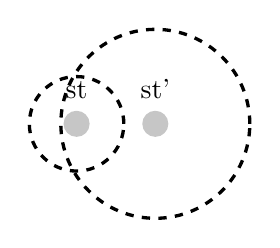
\begin{tikzpicture}
		\begin{scope}[very thick,dashed]
		\draw (0,1) circle (.6cm);
		\draw (0,1) node[circle,fill=gray!45,label=above:st]{};
		\draw (1,1) circle (1.2cm);t
		\draw (1,1) node[circle,fill=gray!45,label=above:st']{};
		\end{scope}
	\end{tikzpicture}
\end{figure}
		
\begin{figure}
    \caption{Link spoofing: Case 4} \label{chap3case4} 
    \centering
	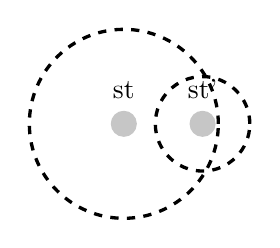
\begin{tikzpicture}
		\begin{scope}[very thick,dashed]
		\draw (0,1) circle (1.2cm);
		\draw (0,1) node[circle,fill=gray!45,label=above:st]{};
		\draw (1,1) circle (0.6cm);
		\draw (1,1) node[circle,fill=gray!45,label=above:st']{};
		\end{scope}
	\end{tikzpicture}

\end{figure}

<<<<<<< HEAD
\emph{Case 3}: $R_{st} \le dist(st,st')$ and $R_{st'} \ge dist(st,st')$. Let's call $\delta_d = dist(st,st') - R_{st}$, we calculate the message traveling time between $n$ and $n'$ as follows: 
\begin{equation*}
\begin{split}
		t(n') - t_n \ge \frac 1 {c}(dist(n,m) + dist(m', n')) + (t(m') - t(m)) \\ \Leftrightarrow
		t(n') - t_n \ge 2 \times \frac 1 {c}(dist(n,m)) + \delta_{tp}\\ \Leftrightarrow
		t(n') - t_n \ge 2 \times \frac 1 {c} (R_{st} + \delta_d) + \delta_{tp} \\ \Leftrightarrow
		2 \times \frac 1 {c} R_{st} + \delta_{tp} \ge 2 \times \frac 1 {c} (R_{st} + \delta_d ) + \delta_{tp} \\ \Leftrightarrow
		0 \ge \delta_{d} 
\end{split}
\end{equation*}
The only possible case is $\delta_{d}$ equals zero. It is too trivial. Otherwise, a fast relay attack occurs at the side from $st$ to $st'$. Case 3 is presented at figure~\ref{chap3case3}.

\emph{Case 4}: $R_{st} \ge dist(st,st')$ and $R_{st'} \le dist(st,st')$. This similarly happens as in case 3. If $R_{st}$ is much larger than $dist(st,st')$, then a fast relay attack occurs at the side from $st'$ to $st$. This is a undesirable result of time-based neighbour discovery protocols. Case 4, hence, is presented at figure~\ref{chap3case4}. $\qed$

=======
\emph{Case 3}: $R_{st} \le dist(st,st')$ and $R_{st'} \ge dist(st,st')$. Let's call $\Delta_d = dist(st,st') - R_{st}$, we calculate the message traveling time between $n$ and $n'$ as follows: 
\begin{equation*}
\begin{split}
		\tau_{n'} - \tau_{n} \ge \frac 1 {c}(dist(n,m) + dist(m', n')) + (\tau_{m'} - \tau_{m}) \\ \Leftrightarrow
		\tau_{n'} - \tau_{n} \ge 2 \times \frac 1 {c}(dist(n,m)) + \delta_{tp}\\ \Leftrightarrow
		\tau_{n'} - \tau_{n'} \ge 2 \times \frac 1 {c} (R_{st} + \Delta_d) + \delta_{tp} \\ \Leftrightarrow
		2 \times \frac 1 {c} R_{st} + \delta_{tp} \ge 2 \times \frac 1 {c} (R_{st} + \Delta_d ) + \delta_{tp} \\ \Leftrightarrow
		0 \ge \delta_{d} 
\end{split}
\end{equation*}
The only possible case is $\Delta_{d}$ equals zero. It is too trivial. Otherwise, a fast relay attack occurs at the side from $st$ to $st'$. Case 3 is presented at figure~\ref{chap3case3}.

\emph{Case 4}: $R_{st} \ge dist(st,st')$ and $R_{st'} \le dist(st,st')$. Presented at the figure~\ref{chap3case4}, it similarly happens as case 3. If $R_{st}$ is much larger than $dist(st,st')$, then a fast relay attack occurs at the side from $st'$ to $st$. 
>>>>>>> 3d6cc25ad869467a057daa522b35e3cad82b4604
%---------------------------Location-based-----------------------%
\subsubsection*{Location-based authentication test}

We formally describe location-based authentication test using knowledge of participant locations. 

\begin{Proposition}
<<<<<<< HEAD
Consider a weak penetrator model, and location information is confidentially exchanged and stored. Given strands $st, st' \in \mathcal{B}$, $\exists link(st,st', \leftrightarrow)$. If $|loc(st),loc(st')| \le R_{st}$, then $\exists plink(st, st',\leftrightarrow)$. 
=======
Consider a weak penetrator model, and location information is confidentially exchanged and stored. Given strands $st, st' \in \mathcal{B}$, $\exists link(st,st', \rightleftharpoons)$. If $|loc(st),loc(st')| \le R_{st}$, then $\exists plink(st, st',\rightleftharpoons)$. 
>>>>>>> 3d6cc25ad869467a057daa522b35e3cad82b4604
\end{Proposition}

\begin{proof}

Since $|loc(st),loc(st')| = dist(st,st')$, evidently $dist(st,st') \le R_{st}$. Furthermore, similarly to first part of proposition~\ref{samerange} proof, we infer $R_{st'} \ge R_{st}$. As a result, there exists a physical link between $st$ and st'. 

\end{proof}

Note that, without assumption on trusted location information, the location-based protocols may contain flaws in some cases. For instance, $st$ could not address correctly the physical location of $st'$ , then a penetrator use his knowledge about location of $st$ to make a fake link between them. Furthermore, location-based protocols share the same trouble with time-based protocols when analysed in our strong penetrator model. 

%-----------------------------------------------------------------------------------------------------------------------------------------------------------------------------%

\section{Analysis of ADVSIG}

<<<<<<< HEAD
In this section, we analyse ADVSIG protocol to show usefulness of our model. There are two kinds of strands in ADVSIG protocol:
\begin{enumerate}
\item Initiator strand $st = \{\langle st, 1 \rangle,\langle st, 2 \rangle,\langle st, 3 \rangle,\langle st, 4 \rangle\} \\ \in Init[A,t_1,t_3,ASYM\_LINK, SYM\_LINK]$ with trace $<+M_1, -M_2 , +M_3,-M_4>$
\item Responder strand $st' = \{\langle st', 1 \rangle,\langle st', 2 \rangle,\langle st', 3 \rangle,\langle st', 4 \rangle\} \\ \in Resp[B,t_2,t_4,ASYM\_LINK, SYM\_LINK]$ with trace $<-M_1, +M_2 , -M_3,+M_4>$
=======
ADVSIG proposed by INRIA group~\cite{Raffo:2004:ASS:1029102.1029106} is a kind of secure routing protocol fortifying for OLSR \cite{Clausen:2003:OLS:RFC3626}. In this protocol, a node wishes to detect neighbours with bi-directional physical links. The protocol is presented as below. 
\begin{flushleft}
 \emph{M1:} $A \to [B]: \{\O, \O, \tau_0\}_{KA}$\\
 \emph{M2:} $B \to [A]: \{\{"A:ASYM\_LINK", \tau_1\}_{KB}, \O,\tau_1\}_{KB}$\\
\emph{M3:} $A \to [B]: \{\{"B:ASYM\_LINK",\tau_2\}_{KA},\O ,\tau_2 \}_{KA})$\\
 \emph{M4:} $B \to [A] : \{\{"A:SYM\_LINK", \tau_3\}_{KB} ,\{"B:ASYM\_LINK",\tau_2\}_{KA} ,\tau_3\}_{KB})$
\end{flushleft}

Moreover, every valid link state must satisfy a maximum interval $\delta_{max}$ defined by $|T_{Sender} - T_e | < \delta_{max}$ where $T_{Sender}$ is the value clock of the sender, and $T_e$ is the value clock of receiver. 

Provided that the third message does not include the proof from the second one, Responder cannot ensure if Initiator has been received the second message or not. As the result of that, internal attackers can produce the first and third messages to valid a protocol run with Responder. Additionally,  neighbours of Responder could be impacted by this attack due to two-hop sensing mechanism in the OLSR protocol.  Figure~\ref{advsigattack3} outlines an attacking scenario to ADVSIG where there only appears a unidirectional link X $\rightarrow$ B.

In the attack scenario, we assume that $X$ accidentally knows the existence of $B$ out of $X$'s physical signal coverage. By using a high power antenna, $X$ can enlarge its signal range. Then $X$ emits valid messages $M1$ and $M3$ to $B$, this makes $B$ believe a existence of bidirectional link between $B$ and $X$.   

\begin{figure}
		\caption{ADVSIG Attack }\label{advsigattack3}
        \centering
        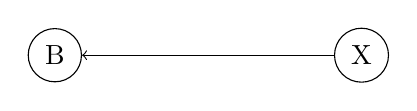
\begin{tikzpicture}
		\draw [<-](1,1) node[anchor=east,circle,draw]{B} to (4.2,1) node[anchor=west,circle,draw]{X};
		\end{tikzpicture}

	    \centering
        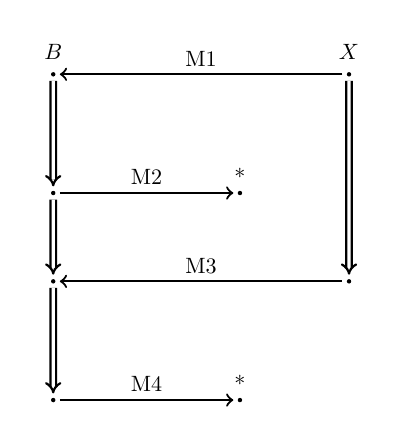
\begin{tikzpicture}[implies/.style={double,double equal sign distance,-implies},
  			dot/.style={shape=circle,fill=black,minimum size=2pt,
  		      inner sep=0pt,outer sep=2pt},thick,scale=0.8, every node/.style={scale=0.8}]
		\matrix[matrix of nodes] {
		  |[dot,label=above:$B$] (B1)| {} & [2cm]|[] (C1)| {}&[1cm] |[dot,label=above:$X$] (X1)| {}\\[1cm]
  		  |[dot] (B2)| {} & [2cm]|[dot,label=above:$*$] (C2)| {}& [1cm]|[dot] (X2)| {}\\[1cm]
  	      |[dot] (B3)| {} & [2cm]|[] (C3)| {}& [2cm]|[dot] (X3)| {}\\[1cm]
 		  |[dot] (B4)| {} & [2cm]|[dot,label=above:$*$] (C4)| {}& [1cm]|[] (X4)| {}\\
		};
		\draw (X1) edge[->] node[above] {M1} (B1)
	      edge[implies] (X3); 
		\draw (B2) edge[->] node[above] {M2} (C2)
	      edge[implies,implies-] (B1);
		\draw (B3) edge[<-] node[above] {M3} (X3)
    	  edge[implies,implies-] (B2);
		\draw (B4) edge[->] node[above] {M4} (C4)
    	  edge[implies,implies-] (B3);
		\end{tikzpicture}

\end{figure}

We analyse ADVSIG protocol to show usefulness of our model. There are two kinds of strands in ADVSIG protocol:
\begin{enumerate}
\item Initiator strand $st =  \{\langle st, 1 \rangle,\langle st, 2 \rangle,\langle st, 3 \rangle,\langle st, 4 \rangle\}\\ \in Init[A,\tau_1,\tau_3]$ with trace $<+M_1, -M_2 , +M_3,-M_4>$
\item Responder strand $st' = \{\langle st', 1 \rangle,\langle st', 2 \rangle,\langle st', 3 \rangle,\langle st', 4 \rangle\} \\ \in Resp[B,\tau_2,\tau_4]$ with trace $<-M_1, +M_2 , -M_3,+M_4>$
>>>>>>> 3d6cc25ad869467a057daa522b35e3cad82b4604
\end{enumerate}

Protocol assumption: 
\begin{itemize}
\item ps1: $|T_{sender} - T_e| < \delta_{max}$
\item ps2: Time synchronisation mechanism is set on participants.
\end{itemize}

\subsubsection*{Initiator's Guarantee} 

The initiator states the guarantee as follows.

<<<<<<< HEAD
Suppose $\mathcal{B}$ is a wireless bundle. Under the conditions $ps1, ps2$, if $\mathcal{B}$ contains a strand $st \in Init[A,t_1,t_3,ASYM\_LINK, SYM\_LINK]$ with $\mathcal{B} -height$ 4, then $\mathcal{B}$ contains a strand $st' \in Resp[B,t_2,t_4,ASYM\_LINK, SYM\_LINK]$ with $\mathcal{B} -height$ 4, and there exists a $plink(st,st',\leftrightarrow)$. 

Mechanically, to find out if the statement is correct or not, we start asserting the logical link guarantee between two participants. 
 
\emph{Logical link guarantee}: At first, we search for a DE edge with an identification factor:
\begin{itemize}
\item The edge $\langle st, 1 \rangle \Rightarrow \langle st, 2 \rangle$ does not contain any identification factor in the challenge message. 
\item The edge $\langle st, 3 \rangle \Rightarrow \langle st, 4 \rangle$ : $term(\langle st, 3 \rangle)$ contains a clear-form identification factor which is response's name $B$ and a timestamp $t_2$, all signed by A's private key, and $term(\langle st, 4 \rangle)$ embodies the a clear-form provable component $\{\{ "A:SYM\_LINK", t_3\}_{KB} ,\{ "B:ASYM\_LINK",t_2\}_{KA} ,t_3\}_{KB}$.
\end{itemize}

The edge $\langle st, 3 \rangle \Rightarrow \langle st, 4 \rangle$ satisfies the authentication logical link test. Therefore, A can verify a logical link between A and B, and B is a regular party. To find out if there exists $plink(st,st,\leftrightarrow)$, we apply the time-based authentication test. 

\emph{Physical link guarantee}: To verify the distance between $st$ and $st'$, we apply the time-based authentication test for the edge $\langle st, 3 \rangle \Rightarrow \langle st, 4 \rangle$. The test concludes that if $(t(\langle st, 4 \rangle) - t(\langle st, 3 \rangle)) \div 2 \le R_{st} \div c$ + $\delta_{tp} \div 2$ (1) then $\exists plink(st,st', \leftrightarrow)$. 

Basing on assumption ps1 and ps2, we calculate the message traveling time from node $\langle st, 3 \rangle$ to $\langle st, 4 \rangle$:
\begin{equation*}
\label{equation1}
\begin{split}
t(\langle st,4\rangle) - t(\langle st, 3 \rangle) = \\
(t(\langle st', 3 \rangle) - t(\langle st, 3 \rangle)) + \\
(t(\langle st', 4 \rangle) - t(\langle st', 3 \rangle)) + \\
(t(\langle st, 4 \rangle) - t(\langle st', 4 \rangle)) \\
\Rightarrow t(\langle st,4\rangle) - t(\langle st, 3 \rangle) \le 2 \times \delta_{max} + \delta_{tp} (2)
=======
Suppose $\mathcal{B}$ is a wireless bundle. Under the conditions $ps1, ps2$, if $\mathcal{B}$ contains a strand $st \in Init[A,\tau_1,\tau_3]$ with $\mathcal{B} -height$ 4, then $\mathcal{B}$ contains a strand $st' \in Resp[B,\tau_2,\tau_4]$ with $\mathcal{B} -height$ 4, and there exists a $plink(st,st',\rightleftharpoons)$. 

Mechanically, to find out if the statement is correct or not, we start asserting the logical link guarantee between two participants. Let's call node $n_1$,  $n_2$, $n_3$ and $n_4$ be $\langle st,1\rangle$, $\langle st,2\rangle$, $\langle st,3\rangle$, and $\langle st,4\rangle$ respectively. 
 
\emph{Logical link guarantee}: At first, we search for a DE edge with an identification factor:
\begin{itemize}
\item The edge $n_1 \Rightarrow n_2$ does not contain any identification factor in the challenge message. 
\item The edge $n_3 \Rightarrow n_4$ : $term(n_3)$ contains a clear-form identification factor which is response's name $B$ and a timestamp $\tau_2$, all signed by A's private key, and $term(n_4)$ embodies the a clear-form provable component $\{\{ "A:SYM\_LINK", \tau_3\}_{KB} ,\{ "B:ASYM\_LINK",\tau_2\}_{KA} ,\tau_3\}_{KB}$.
\end{itemize}

The edge $n_3 \Rightarrow n_4$ satisfies the authentication logical link test. Therefore, $A$ can verify a logical link between $A$ and $B$, and $B$ is a regular party. To find out if there exists $plink(st,st,\rightleftharpoons)$, we apply the time-based authentication test.  

\emph{Physical link guarantee}: To verify the distance between $st$ and $st'$, we apply the time-based authentication test for the edge $n_3 \Rightarrow n_4$. The test concludes that if $(t_{n_4} - t_{n_3}) \div 2 \le R_{st} \div c$ + $\delta_{tp} \div 2$ (1) then $\exists plink(st,st', \rightleftharpoons)$. Let's call node $n'_3$ and $n'_4$ be $\langle st',3\rangle$, and $\langle st',4\rangle$ respectively. 

Basing on assumption ps1 and ps2, we calculate the message traveling time from node $n_3$ to $n_4$:
\begin{equation*}
\label{equation1}
\begin{split}
t_{n_4} - t_{n_3} = \\
(t_{n'_3} - t_{n_3}) + (t_{n'_4} - t_{n'_3}) + (t_{n_4} - t_{n'_4}) \\
\Rightarrow t_{n_4} - t_{n_3} \le 2 \times \delta_{max} + \delta_{tp} (2)
>>>>>>> 3d6cc25ad869467a057daa522b35e3cad82b4604
\end{split}
\end{equation*}

 Let $2\times(1) - (2)$, we have
\begin{equation*}
\label{equation2}
\begin{split}
	R_{st} \div c - \delta_{max} \ge 0 (3)
\end{split}
\end{equation*}

<<<<<<< HEAD
If inequality (3) holds, then $\exists plink(st,st', \leftrightarrow)$. $\qed$
=======
If inequality (3) holds, then $\exists plink(st,st', \rightleftharpoons)$. $\qed$
>>>>>>> 3d6cc25ad869467a057daa522b35e3cad82b4604
  
\subsubsection*{Responders Guarantee}

The initiator states the guarantee as follows.

<<<<<<< HEAD
Suppose $\mathcal{B}$ is a wireless bundle. Under the conditions $ps1, ps2$, if $\mathcal{B}$ contains a strand $st' \in Resp[A,t_1,t_3,ASYM\_LINK, SYM\_LINK]$ with $\mathcal{B} -height$ 4, then $\mathcal{B}$ contains a strand $st \in Init[B,t_2,t_4,ASYM\_LINK, SYM\_LINK]$ with $\mathcal{B} -height$ 4, and there exists a $plink(st,st',\leftrightarrow)$. 

The proof of this statement is quite identical to initiator's guarantee. However, when looking for a double logical link, regrettably, we cannot find any logical link test edge in the responder strand. As a result, $B$ can be a victim of spoofing attack. $\qed$ 
 
\subsubsection*{Link spoofing attack on ADVSIG} 

Formally describing, let's call node $n_1$ and $n_2$ be $\langle st, 1 \rangle$ and $\langle st, 3 \rangle$ respectively. Since $n_1$ and $n_3$ do not contain any proof of reception, they possibly lie on B strand. Definitely, they do. 

When X accidentally knows the existence of B but it cannot listen to B, X persuades B that B will own a double physical link with X. Thus, penetrator X strand is: 
\begin{center}
$st_x =$ $\{(M_1,loc(\langle st_X,1\rangle),t(\langle st_X,1\rangle), R_M),(M_3,loc(\langle st_X,2\rangle),t(\langle st_X,2\rangle), R_M)\}$ $\in$ \\
$Init[X,t_1,t_2,t_3,ASYM\_LINK,SYM\_LINK]$ with trace $<+M_1,+M_3>$.
\end{center}
=======
Suppose $\mathcal{B}$ is a wireless bundle. Under the conditions $ps1, ps2$, if $\mathcal{B}$ contains a strand $st' \in Resp[A,\tau_1,\tau_3]$ with $\mathcal{B} -height$ 4, then $\mathcal{B}$ contains a strand $st \in Init[B,\tau_2,\tau_4]$ with $\mathcal{B} -height$ 4, and there exists a $plink(st,st',\rightleftharpoons)$. 

The proof of this statement is quite identical to initiator's guarantee. However, when looking for a bidirectional logical link, regrettably, we cannot find any logical link test edge in the responder strand. As a result, $B$ can be a victim of spoofing attack. $\qed$ 
 
\subsubsection*{Link spoofing attack on ADVSIG} 

Since $n_1$ and $n_3$ do not contain any proof of reception, they possibly lie on $X$ strand. Definitely, they do. 

When $X$ accidentally knows the existence of $B$ but it cannot listen to $B$, $X$ persuades $B$ that $B$ will own a bidirectional physical link with X. Thus, penetrator X strand is: 
\begin{flushleft}
$st_x = \{(M_1,loc(\langle st_X,1\rangle),\tau_{x1}, R_M) ,(M_3,loc(\langle st_X,2\rangle)$ \\ $,\tau_{x3}, R_M)\}$ $\in$ 
 $Init[X,\tau_{x1},\tau_{2},\tau_{x3}]$ with trace $<+M_1,+M_3>$.
\end{flushleft}

Furthermore, we found a similar flaw in the work~\cite{Adnane20131159}. The authors proposed a trusted-based security for OLSR protocols where all participants must trust together. However, internal attackers can successfully create a fake bidirectional physical link to a target as they do in ADVSIG. 
>>>>>>> 3d6cc25ad869467a057daa522b35e3cad82b4604

\section{Conclusion}

This chapter has addressed a serious problem of current neighbour discovery protocols that have not introduced before. The problem comes when participants use wireless interfaces with different signal power, that leads the ND protocols cannot correctly verify the distance between participants.  

We extended the original strand space model to be able to analyse secure neighbour protocols. To achieve this, we modified the model so that it becomes possible to take into account some physical properties including timestamp, location, and signal propagation. The penetrator model has been adapted in consequence. Thank our model, time-based, even location-based neighbour discovery techniques were formally proved that they would not guarantee the existence of physical bidirectional links. 

Aforementioned works on this topic, mainly apply existing verification tools initially. We rather chosen to define a dedicated formalism able to model physical properties in neighbour discovery protocols in a natural manner, and the results obtained so far seems promising. Concerning future work, we will first try to extend the model in order to capture mobility and network topology. In a second step, we plan to study how we could automate the analysis procedure.
 
%\input{./Chapters/Chapter5} 
%% Chapter Template

\chapter{Conclusion and Future Work} % Main chapter title

\label{Chapter6} % Change X to a consecutive number; for referencing this chapter elsewhere, use \ref{ChapterX}

\lhead{Chapter 6. \emph{Conclusion and Future Work}} % Change X to a consecutive number; this is for the header on each page - perhaps a shortened title

%----------------------------------------------------------------------------------------
%	SECTION 1
%----------------------------------------------------------------------------------------
This chapter summaries the thesis results, discusses a few limitation, and introduces possible future work. 

\section{Summary}

In this thesis, we have investigated three critical problems of current security protocol design in IoT, particularly in secure device pairing and neighbour discovery protocol, that received very little attention on physical security properties, physical attacks, and formal analysis. As our first contribution, we introduced our novel pairing protocol that is secure and efficient than other competitions in communication cost, but remains the attack probability. Precisely, it only uses two messages on wireless channels, and one on a public out-of-band channel. Additionally, an implementation on an embedded system was conducted to show the usefulness of our protocol. Meanwhile, we found attacks in some existing secure pairing protocols, some of which are using in commercial products. 

We investigated that secure device pairing are strongly affected by many physical aspects that cannot be resolved by any classical formal method. Taking the obstacles into account, our model as the second contribution is constructed on famous Strand Spaces with supplement notations of channel. Our model also captures both physical attacks and specific attacks on secure channels. Along with the improved model, we proposed a procedure that transforms a model in our extended formalism of an initial protocol using OOB channels to a model in original Strand Spaces of a protocol that does not use any OOB channel. In addition, the translation exactly preserves security properties of initial protocol. As a result, our translation allows us to formalise out-of-band channels-based protocols in current automatic verification tools. 

Our another main contribution is a study of current neighbour discovery protocols in wireless network, and formal models for such protocols. We spotted a problem where signal range of two principals is different. As a result, when analysed in our model, the time-based, or distance-based schemes do not exactly provide link agreement among principals. Finally, some protocols have been analysed in our model as our proof of concept. 
 
Our final contribution was proposing a new secure and robust bootstrapping scheme for constrain devices. Our scheme takes more advantages than other competitors since it does not require pre-shared key, implanted public keys, and even PKI system. Furthermore, it still works when a home gateway is down, and a new thing is second-handed stuff. 

\section{Perspective}

In Chapter 3, our model takes reasonable assumptions on which both principals in the protocol are honest, and out-of-band channels are at least authenticated. Hence, to take internal attacks into account, our model should express the attacks at a specific probability.

As introduced in Chapter 4, our formal model successfully reasons about physical properties-related protocols through specific examples. Currently, the model focuses on some particular physical aspects, yet does not include device mobility. For further work, we continue enlarging our model to cover dynamic networks, and topology aspects as well. After successfully reasoning about secure neighbour discovery protocols, we keep going to adapt our model to secure routing protocols, or secure protocols in vehicle networks. We strongly believe that our model achieves more promising results. 

In chapter 5, our bootstrap framework is partly implemented in a prototype hardware. So, we are going to completely deploy the scheme using adaptation of current authentication systems such as RADIUS, PANA on 802.15.4 wireless technology. Obviously, this work is not too complicated to be complete. As a consequence, the framework will be comprehensively evaluated security, usability, and performance when fully constructed. 

As a fact of that, manual proving task is prone to errors, we should looking for a way to implement our model into an automatic proving tool. In literature, Song~\cite{Song:1999:ANE:794199.795118} proposed an algorithm based on Strand Spaces model. And, the algorithm was also deployed in a tool named Athena. Unfortunately, we cannot access this tool since its authors do not publish their source code. Certainly, rebuilding the source code will take a plenty of time, so this work is planned in close future. 

In long-term, we will bind all separated and unfinished pieces of current work. Moreover, an automatic or assistant proving tool is our first main goal. The tool, of course, will be fully adapted to study wider wireless protocol families, rather than two protocols discussed in this thesis. Visualising attacks could be interesting as well. Along with developing tools, a complete bootstrapping framework for IoT applications will be discussed more to become an industrial standard. 
 


%----------------------------------------------------------------------------------------
%	THESIS CONTENT - APPENDICES
%----------------------------------------------------------------------------------------

\addtocontents{toc}{\vspace{2em}} % Add a gap in the Contents, for aesthetics

\appendix % Cue to tell LaTeX that the following 'chapters' are Appendices

% Include the appendices of the thesis as separate files from the Appendices folder
% Uncomment the lines as you write the Appendices

% Appendix Template

\chapter{Strand Spaces Model}\label{AppexA} % Main appendix title

\label{Strand Spaces Model} % Change X to a consecutive letter; for referencing this appendix elsewhere, use \ref{AppendixX}

\lhead{Appendix A. \emph{Strand Spaces Model}} % Change X to a consecutive letter; this is for the header on each page - perhaps a shortened title

In 1997, Fabrega, Herzog and Gutman developed a new method to prove a protocol if it achieves authentication and secrecy properties or not. First published internally as a technical report, the work went out public in a conference paper ~\cite{674832} in a year later. Following this approach, the authors continued maturing their model. Basic Strand Spaces theory was extended with \emph{honest idea}~\cite{Thayer:1998:HIS:794198.795096} which allows to learn general principles that limit penetrators' capabilities. After that, \emph{mixed strands}~\cite{Thayer:1999:MSS:794199.795113} was proposed to study problems of mixed protocols. One huge milestone of Strand Spaces theory is \emph{authentication tests}~\cite{Guttman:2002:ATS:568264.568267} proposed in 2000. In a study of cryptographic protocols, authors realized that after emitting a message containing a new value, a participant receives a cryptographic form of this value, this must exist a regular participant of the protocol sent it. This scheme, so called an authentication test, works as a powerful tool to minimise work of proving, and straightforwardly give results of authentication protocols. From 2002 to 2007, Strand Spaces theory was enriched with \emph{shape of bundle, skeleton and homomorphism}~\cite{Doghmi:2007:SHS:1230146.1230260}. These theories study about a sort of protocols that share the same forms. Current developments of Strand Spaces are focusing on various of types of protocols such as TLS~\cite{Kamil:2011:ATS:2590701.2590707}, location-awareness protocols~\cite{Thayer:2010aa}, and DH protocols~\cite{1212716}. 

<<<<<<< HEAD
In our work, we continue adding more ingredients in Strand Spaces to get more juice in wireless context. We select and present some extensions that we will use in our model. Other extensions objective closely to our work will be presented in related work of chapter 3 and 4. Definitions used in thesis are referred from \cite{674832}, \cite{Guttman:2002:ATS:568264.568267} and~\cite{Doghmi:2007:SHS:1230146.1230260}. 
=======
Definitions used in thesis are referred from \cite{674832}, \cite{Guttman:2002:ATS:568264.568267} and~\cite{Doghmi:2007:SHS:1230146.1230260}. Furthermore, to make readers conformable with the theory, the Needham-Schroeder(NS) protocol~\cite{Needham:1978:UEA:359657.359659} presented below is used as an example through this part. 

\begin{enumerate}
\item $A \rightarrow B$: $\{N_a, A\}_{K_B}$
\item $B \rightarrow A$: $\{N_a,N_b, B\}_{K_A}$
\item $A \rightarrow B$: $\{N_b\}_{K_B}$
\end{enumerate}
>>>>>>> 3d6cc25ad869467a057daa522b35e3cad82b4604

\section{Fundamental Theory}

A security protocol is an ordered sequence of messages that participants exchange in a protocol. Let $\mathcal{A}$ a set of possible messages intentionally transferred in a security protocol, and elements of this set are referred to as \textit{terms}. Additionally, the set $\mathcal{A}$ is algebra freely generated from of a set of text terms $\mathcal{T}$ and a set of cryptographic keys $\mathcal{K}$ by means of concatenation and encryption. While $\mathcal{T}$ contains textual information such as nonces, $\mathcal{K}$ contains symmetric and/or asymmetric cryptographic keys. The two sets $\mathcal{T}$ and $\mathcal{K}$ are disjoint. 

\begin{Definition} $\emph{Compound terms}$ are generated by two operators
\begin{itemize}
	\item encr: $\mathcal{K} \times \mathcal{A} \rightarrow \mathcal{A}$ representing encryption
	\item join: $\mathcal{A} \times \mathcal{A} \rightarrow \mathcal{A}$ representing concatenation
\end{itemize}
\end{Definition}

<<<<<<< HEAD
For convention, from now we express the concatenation of two term $t$ and $t'$ as $\textit{tt'}$ and encryption of term $t$ with key $K$ as $\{t\}_K$. We continue defining a relation, \textit{subterm relation}, on the set $\mathcal{A}$. 
=======
For convention, from now we express the concatenation of two term $t$ and $t'$ as $\textit{t,t'}$ and encryption of term $t$ with key $K$ as $\{t\}_K$. We continue defining a relation, \textit{subterm relation}, on the set $\mathcal{A}$. 
>>>>>>> 3d6cc25ad869467a057daa522b35e3cad82b4604

\begin{Definition} The $\emph{subterm relation}$ $\sqsubseteq$ over $\mathcal{A}$ is defined inductively as: 
	\begin{itemize}
		\item $a \sqsubseteq t $ for $t \in \mathcal{T}$   iff $a = t $
		\item $a \sqsubseteq key $ for $t \in \mathcal{K}$   iff $a = key $
		\item $a \sqsubseteq gh $ iff $a \sqsubseteq gh, a \sqsubseteq h $ or $ a= h $
		\item $a \sqsubseteq \{g\}_K $ iff $a \sqsubseteq g $ or $a = \{g\}_K$
	\end{itemize} 
\end{Definition}

<<<<<<< HEAD
Remark that, $t_1\sqsubseteq t$ means $t_1$ is a subterm of $t$. A \textit{subterm} is just a term that can be easily extracted from a term with an appropriate key. Taking the Needham-Schroeder \cite{Needham:1978:UEA:359657.359659}(NS) protocol as an example, initiator A starts sending a message (or a $term$) of the form $\{N_a,A\}_{PK_B}$ to intentional responder B, where $PK_B$ is the public key of B. Subterms of term $\{N_a,A\}_{PK_B}$ could be $N_a, A$, or $\{N_a,A\}_{PK_B}$. Since $PK_B$ is a key, $PK_B \not\sqsubseteq \{N_a,A\}_{PK_B}$, except a case when $PK_B$ is in a value of this message. 
=======
Remark that, $t_1\sqsubseteq t$ means $t_1$ is a subterm of $t$. A \textit{subterm} is just a term that can be easily extracted from a term with an appropriate key. In NS protocol, initiator $A$ starts sending to intentional responder $B$ a message (or a $term$) of the form $\{N_a,A\}_{K_B}$ where $K_B$ is the public key of $B$. Subterms of term $\{N_a,A\}_{K_B}$ could be $N_a, A$, or $\{N_a,A\}_{K_B}$. Since $K_B$ is a key, $K_B \not\sqsubseteq \{N_a,A\}_{K_B}$, except a case when $K_B$ is in a value of this message. 
>>>>>>> 3d6cc25ad869467a057daa522b35e3cad82b4604

Terms are extended to $\textit{signed term}$ including a positive represented to a transmission, and a negative one represented to a reception. 

\begin{Definition} A $\emph{signed term}$ is a pair $\langle\delta,a\rangle$ with $a \in A$ and $\delta$ one of the symbols $+,-$. We will write a signed term as $+t$ or $-t$. $(\pm A)^*$ is the set of finite sequences of signed terms. We denote a typical element of $(\pm A)^*$ by $\langle \delta_1,a_1\rangle,.....,\langle\delta_n,a_n\rangle$.
\end{Definition}

<<<<<<< HEAD
A sequence of sending and receiving messages in a protocol is called $strand$, and a set of strands is called $\textit{Strand Spaces}$. 

When modeling a protocol, the strand of a principal is a sequence of events as seen by that principal in a particular protocol run and in a particular instance of role. For example, the strand of the initiator for the NS protocol is $\langle+\{N_a,A\}_{PK_B}, -\{N_a,N_b\}_{PK_A},+\{N_b\}_{PK_B} \rangle$. The first event is emission of $\{N_a,A\}_{PK_B}$ followed by reception of $\{N_a,N_b\}_{PK_A}$ and so on. 
=======
Note that, the unsigned term is the term without direction. For example, a signed term $+t$ has direction $+$, and an unsigned term $t$. 

A sequence of sending and receiving messages in a protocol is called $strand$, and a set of strands is called $\textit{Strand Spaces}$. 

When modeling a protocol, the strand of a principal is a sequence of events as seen by that principal in a particular protocol run and in a particular instance of role. For example, the strand of the initiator for the NS protocol is $\langle+\{N_a,A\}_{K_B}, -\{N_a,N_b\}_{K_A},+\{N_b\}_{K_B} \rangle$. The first event is emission of $\{N_a,A\}_{K_B}$ followed by reception of $\{N_a,N_b\}_{K_A}$ and so on. 
>>>>>>> 3d6cc25ad869467a057daa522b35e3cad82b4604

\begin{Definition}
A $\emph{Strand Spaces}$ is a set $\Sigma$ with a trace mapping tr: $\Sigma \rightarrow (\pm A)^*$.
\end{Definition}

For a Strand Spaces $\Sigma$:

	\begin{itemize}
		\item A node is a pair $\langle s,i\rangle$, with $s \in \Sigma$ and i an integer satisfying $1\leq i \leq length(tr(s))$. The set of nodes is denoted by $\mathcal{N}$. We will say the node $n= \langle s,i\rangle$ belongs to the strand s. Clearly, every node belongs to a unique strand. 

		\item If $n= \langle s,i \rangle \in \mathcal{N}$ then $index(n) = i$ and $strand(n)=s$. Define $term(n)$ to be $(tr(s))_i$, i.e. the $i^{th}$ signed term in the trace of $s$. Similarly, $uns\_term(n)$ is $((tr(s))_i)_2$, i.e. the unsigned part of the $i^{th}$ signed term in the trace of $s$

		\item If $n,n' \in \mathcal{N}, n \rightarrow n'$ mean $term(n) = +a$ and $term(n') = +a$ It means that node $n$ sends the message $a$ which is received by $n'$, creating a causal link between their strands.

		\item If $n,n' \in \mathcal{N}, n \Rightarrow n'$ mean $n$ and $n'$ occur on the same strand with $index(n)=index(n') -1 $. It expresses that $n$ is an immediate causal predecessor of $n'$ on the strand. 
		
		\item $n \Rightarrow^+ n'$ to mean that $n$ precedes $n'$ (not necessarily immediately) on the same strand.
			
		\item $m \Rightarrow^* n$ means $m \rightarrow n_1 \Rightarrow m_2 \rightarrow n_2 \Rightarrow ......m_k \rightarrow n$ where $n_i, m_i$, and n stand on the same or different strands. A \emph{path} created by $m \Rightarrow^* n$ forms a connectivity subgraph in the bundle. 

		\item An unsigned term $t$ $occurs$ in $n \in \mathcal{N}$ if $t \sqsubseteq term(n)$.

		\item An unsigned term $t$ $originates$ on $n \in \mathcal{N}$ iff:$term(n)$ is positive, $t \sqsubseteq term(n)$, and whenever $n$ precedes $n$ on the same strand, $t \not\sqsubseteq term(n)$.

		\item An unsigned term $t$ is $\textit{uniquely originating}$ iff $t$ originates on a unique $n \in \mathcal{N}$ 

	\end{itemize}
<<<<<<< HEAD
=======

Let  the Initiator strand be $st = \langle +\{N_a,A\}_{K_B}, -\{N_a,N_b\}_{K_A},+\{N_b\}_{K_B} \rangle$, and the responder strand be $st' = \langle -\{N_a,A\}_{K_B}, +\{N_a,N_b\}_{K_A},-\{N_b\}_{K_B} \rangle$.

The first node of Initiator strand is $\langle st,1 \rangle = +\{N_a,A\}_{K_B}$. Moreover, $\langle st,1 \rangle \Rightarrow \langle st,2 \rangle$ means node $\langle st,1 \rangle$ is a causal predecessor of node $\langle st,2 \rangle$. $N_a$ occurs in $term(\langle st,1 \rangle)$. Additionally, since sign of $\langle st,1 \rangle$ is positive, and there does not exist any predecessor of $\langle st,1 \rangle$, $N_a$ uniquely originates at $\langle st,1 \rangle$.  
>>>>>>> 3d6cc25ad869467a057daa522b35e3cad82b4604
	
Let $\mathcal{N}$ be a set of nodes, and let $\mathcal{E}$ be the union of the sets of $\rightarrow$ and $\Rightarrow$ edges. A directed graph $\mathcal{G}$ has a structure $\mathcal{G} = \langle \mathcal{N},\mathcal{E}\rangle$. A $bundle$ is a finite subgraph of this graph in which the edges express casual dependencies of the nodes.

\begin{Definition} Suppose $\mathcal{N_B}$ be a subset of $\mathcal{N}$, and $\mathcal{E_B}$ be a subset of $\mathcal{E}$. Let $\mathcal{B} = \langle \mathcal{N_B},\mathcal{E_B}\rangle$ be a subgraph of $\mathcal{G}$. $\mathcal{B}$ is a $\emph{bundle}$ if :
\begin{enumerate}
\item $\mathcal{N_B}$ and $\mathcal{E_B}$ are finite
\item If $n \in \mathcal{N_B}$ and $term(n)$ is negative, then there is a unique $n'$ such that $ n' \rightarrow n \in \mathcal{E_B}$
\item If $n \in \mathcal{N_B}$ and $n \Rightarrow n'$ then $n \Rightarrow n' \in \mathcal{E_B}$ 
\item $\mathcal{B}$ is acyclic
\end{enumerate}
\end{Definition}

<<<<<<< HEAD
Remark: Guttman implicitly expressed that when a node transmits a message, there is more than one (or none) receiving node of the message. However, we hardly see more than two receptions in their studies. 
=======
The graph consisting of the Initiator strand $st$ and responder strand $st'$ is called a NS bundle. Remarking that Guttman implicitly expressed that when a node transmits a message, there is more than one (or none) receiving node of the message. However, we hardly see more than two receptions in their studies. 
>>>>>>> 3d6cc25ad869467a057daa522b35e3cad82b4604

\begin{Definition}
A node $n$ belongs to a bundle $\mathcal{B} = \langle \mathcal{N_B},\mathcal{E_B}\rangle$ , written $n \in \mathcal{B}$ if $n \in \mathcal{N_B}$. The $\mathcal{B} -height$ of a strand $s \in \mathcal{B}$ is the largest $i$ such that $\langle s,i \rangle \in \mathcal{B}$. 
\end{Definition}

For instance, in NS protocol, $\mathcal{B}-height$ of initiator strand is 3, similarly $\mathcal{B}-height$ of responder strand is also 3.

%introduce component
\section{Component, Authentication Tests}

After introducing Strand Spaces fundamental theory, basing on the fact that security authentication protocols usually use specific challenge-response methods to obtain goals, Thayer et al\cite{authenticationtests} continued publishing a theory of $\textit{authentication tests}$ as a tool to prove security properties for protocols easily. 

\begin{Definition}
 A term $t'$ is called a \emph{component} of term $t$ if $t'$ cannot be split to another term $t''$, and $t$ is built by concatenating $t'$ with arbitrary terms.
\end{Definition}

Conveniently, we refer the example of Thayer\cite{Thayer:2010aa}. If we have a term like $B\{N_aK\{KN_b\}_{K_B}\}_{K_A}N_a$, then it contains three components: $B, \{N_aK\{KN_b\}_{K_B}\}_{K_A}$, and $N_a$. 
 
\begin{Definition}
 For a strand s, a term t is \emph{new} at $n = \langle s,i\rangle$ if t is a component of term(n), but t is not a component of node $\langle s,j\rangle$ for every $j<i$. 
\end{Definition}

<<<<<<< HEAD
\begin{Definition} Suppose that $n \in \mathcal{B}$ is positive, $\emph{a}$ $\in \mathcal{A}$ is a subterm of $term(n)$. The edge $n \Rightarrow^+ n'$ is a \emph{transformed edge} for $\emph{a}$ if there exits a negative node $n' \in \mathcal{B}$, and there is a new component $t_2$ of $n'$ such that $a \sqsubseteq t_2$.
\end{Definition}

Respectively, \textit{a transforming edge} is denoted. 
=======
Taking NS protocol as an example, the component $\{N_a,N_b,B\}_{K_B}$ is new at node $\langle st,2 \rangle$ since it is clearly not a component of $\langle st,1 \rangle$. 

\begin{Definition} Suppose that $n \in \mathcal{B}$ is positive, $\emph{a}$ $\in \mathcal{A}$ is a subterm of $term(n)$. The edge $n \Rightarrow^+ n'$ is a \emph{transformed edge} for $\emph{a}$ if there exits a negative node $n' \in \mathcal{B}$, and there is a new component $t_2$ of $n'$ such that $a \sqsubseteq t_2$.
\end{Definition}

Respectively, \textit{a transforming edge} is denoted.
>>>>>>> 3d6cc25ad869467a057daa522b35e3cad82b4604

\begin{Definition} Suppose that $n \in \mathcal{B}$ is negative, $\emph{a}$ $\in \mathcal{A}$ is a subterm of $term(n)$. The edge $n \Rightarrow^+ n'$ is a \emph{transforming edge} for $\emph{a}$ if there exits a positive node $n' \in \mathcal{B}$, and there is a new component $t_2$ of $n'$ such that $a \sqsubseteq t_2$.
\end{Definition}

<<<<<<< HEAD
=======
 For example, the edge $\langle st,1\rangle \Rightarrow \langle st,2\rangle$ is a transformed edge for the term $N_a$, and  $\langle st',1\rangle \Rightarrow \langle st',2\rangle$ is a transforming edge for $N_a$. 

>>>>>>> 3d6cc25ad869467a057daa522b35e3cad82b4604
\begin{Definition} 
The edge $n \Rightarrow^+ n'$ is \emph{a test} for $\emph{a}$ $\in \mathcal{A}$ if $\emph{a}$ uniquely originates at $n$, and $n \Rightarrow^+ n'$ is a transformed edge for $\emph{a}$. 
\end{Definition}

<<<<<<< HEAD
\begin{Definition} Suppose that $n, n' \in \mathcal{B}$.
\begin{enumerate}
\item The edge $n \Rightarrow^+ n'$ is \emph{a outgoing test} for $a$ $\sqsubseteq t = \{|h|\}_K$ if it is a test for $a$ in which $K^{-1} \not\in P$, $a$ does not occur in any component of $n$ other than t. Moreover, $t$ is a test component for $a$ in $n$.
\item The edge $n \Rightarrow^+ n'$ is \emph{a incoming test} for $a$ $\sqsubseteq t_1 = \{|h|\}_K$ if it is a test for $a$ in which $K \not\in P$, and $t_1$ is a test component for $a$ in $n'$.
\end{enumerate}
\end{Definition}

Subsequently, authentication tests~\cite{authenticationtests} are provided as powerful and simple tools to guarantee existence of regular strands in a bundle. 

\emph{Authentication Test 1}: Suppose that $n' \in \mathcal{B}$, and $n \Rightarrow^+ n'$ is outgoing test for $\emph{a}$ $\sqsubseteq t$ with $t = term(n)$. Then there exist regular nodes $m,m' \in \mathcal{B}$ such that $t$ is a component of $m$, and  $m \Rightarrow^+m'$ is a transforming edge for $\emph{a}$. In addition that $\emph{a}$ occurs only in component $t_1=\{|h_1|\}_{K_1}$ of $m'$, that $t_1$ is not a proper subterm of any regular component, and that $K^{-1}_1 \not\in P$. There is a negative regular node with $t_1$ as a component. 
=======
The transformed edge $\langle st,1\rangle \Rightarrow \langle st,2\rangle$ is a test for $N_a$ since $N_a$ uniquely originates at $\langle st,1\rangle$. 

\begin{Definition} Suppose that $n, n' \in \mathcal{B}$.
\begin{enumerate}
\item The edge $n \Rightarrow^+ n'$ is \emph{a outgoing test} for $a$ $\sqsubseteq t = \{h\}_K$ if it is a test for $a$ in which $K^{-1} \not\in P$, $a$ does not occur in any component of $n$ other than t. Moreover, $t$ is a test component for $a$ in $n$.
\item The edge $n \Rightarrow^+ n'$ is \emph{a incoming test} for $a$ $\sqsubseteq t_1 = \{h\}_K$ if it is a test for $a$ in which $K \not\in P$, and $t_1$ is a test component for $a$ in $n'$.
\end{enumerate}
\end{Definition}

The transformed edge $\langle st,1\rangle \Rightarrow \langle st,2\rangle$ could be considered as an incoming test for $N_a$. 

Subsequently, authentication tests~\cite{authenticationtests} are provided as powerful and simple tools to guarantee existence of regular strands in a bundle. 

\emph{Authentication Test 1}: Suppose that $n' \in \mathcal{B}$, and $n \Rightarrow^+ n'$ is outgoing test for $\emph{a}$ $\sqsubseteq t$ with $t = term(n)$. Then there exist regular nodes $m,m' \in \mathcal{B}$ such that $t$ is a component of $m$, and  $m \Rightarrow^+m'$ is a transforming edge for $\emph{a}$. In addition that $\emph{a}$ occurs only in component $t_1=\{h_1\}_{K_1}$ of $m'$, that $t_1$ is not a proper subterm of any regular component, and that $K^{-1}_1 \not\in P$. There is a negative regular node with $t_1$ as a component. 
>>>>>>> 3d6cc25ad869467a057daa522b35e3cad82b4604


\emph{Authentication Test 2}: Suppose that $n \in \mathcal{B}$, and $n \Rightarrow^+ n'$ is incoming test for $\emph{a}$ $\sqsubseteq t'$ with $t' = term(n')$. Then there exist regular nodes $m,m' \in \mathcal{B}$ such that $t'$ is a component of $m'$, and  $m \Rightarrow^+m'$ is a transforming edge for $\emph{a}$. 

\begin{Definition} 
<<<<<<< HEAD
A negative node is an \emph{unsolicited test} for $t = \{|h|\}_K$ if $t$ is a test component for any $a$ in $n$ and $K \not\in P$. 
\end{Definition}

\emph{Authentication Test 3}: Suppose that a node $n$ is in a bundle $\mathcal{B}$, and $n$ be an unsolicited test for $t = \{|h|\}_K$, then there exists a positive regular node $m \in \mathcal{B}$ such that $t$ is a component of $m$. 
=======
A negative node is an \emph{unsolicited test} for $t = \{h\}_K$ if $t$ is a test component for any $a$ in $n$ and $K \not\in P$. 
\end{Definition}

\emph{Authentication Test 3}: Suppose that a node $n$ is in a bundle $\mathcal{B}$, and $n$ be an unsolicited test for $t = \{h\}_K$, then there exists a positive regular node $m \in \mathcal{B}$ such that $t$ is a component of $m$. 
>>>>>>> 3d6cc25ad869467a057daa522b35e3cad82b4604
 
The proofs of these authentication tests are out of scope in this part. So if readers eager to deeply understand the proofs, please regard to the paper \cite{Guttman:2002:ATS:568264.568267}.


\section{Shape and Skeleton}

In design protocol, ones always desire that there is only one possible execution of their protocol in any scenario. Nevertheless, there might exist some executions relative to the protocol's assumptions. Actually, the executions of protocols normally have very few essentially different forms that called $shapes$. Then, authentication and secrecy properties can be determined by examining the shapes.

Precisely, a shape is a local execution by honest principals. Partial information about a principal's execution of a protocol is called \emph{skeleton}. Skeletons are partial-ordered structures, or fragments of message sequence chart. Moreover, a skeleton is $realised$ if it is not fragmented, i.e. it contains exactly the regular behavior of some executions. A realised skeleton is a shape if it is minimal. 

A preskeleton describes the regular parts of a set of bundles. Formally presented, preskeleton is defined as follows.
\begin{Definition}[Skeleton]A four-tuple $\mathcal{A} = (node, \preceq, non, unique)$ is a preskeleton if:
	\begin{enumerate}
	\item $node$ is a finite set of regular nodes, $n_1 \in node$ and $n_0 \Rightarrow^+ n_1$ implies $n_0 \in nodes$;
	\item $\preceq$ is a partial ordering on $node$ such that $n_0 \Rightarrow^+ n_1$ imples $n_0 \preceq n_1$;
	\item $non$ is a set of keys where if $K \in non$, then for all $n \in node, K\not\sqsubseteq term(n)$, and for some $n' \in node$, either $K$ or $K^{-1}$ is used in $term(n')$;
	\item $unique$ is a set of atoms where $a \in unique$, for some $n \in node, a \sqsubseteq term(n)$. 
	\end{enumerate}
	A preskeleton $\mathcal{A}$ is a $skeleton$ if in addition:
	\begin{enumerate}
	\item[4'.] $a\in unique$ implies $a$ originates at no more than one $n\in node$. 
	\end{enumerate}
\end{Definition}

\begin{Definition}[Shape] $\mathcal{A}'$ is a $shape$ for $\mathcal{A}$ if (1) some $H : \mathcal{A} \rightarrow \mathcal{A'}$, (2) $\mathcal{A'}$ is realised, and (3) no proper skeleton of $\mathcal(A')$ satisfies (1) and (2). 
\end{Definition}

<<<<<<< HEAD
=======
A strand could be considered as a skeleton. And a bundle could be considered as a shape. Furthermore, a bundle containing a penetrator strand is also a possible shape of the protocol. 

>>>>>>> 3d6cc25ad869467a057daa522b35e3cad82b4604
\section{Penetrator Model}

Original Strand Spaces theory uses Dolev-Yao \cite{dolev-yao} model as its penetrator model. Penetrator's power is built up from two ingredients: initially known keys available to the penetrator, and actions that allows the penetrator manipulates messages. The actions are summarized to discard message, to generate arbitrary messages, to concatenate messages together, and to apply cryptographic operation using available keys. The model is described as follows. 

\begin{Definition} A penetrator trace is \emph{one of the following}:
\begin{itemize}
\item[\textbf{M}.] Text message: $\langle+t\rangle$ where $t \in T$
\item[\textbf{F.}] Flushing: $\langle-g\rangle$ 
\item[\textbf{T.}] Tee: $\langle-g,+g,+g\rangle$
\item[\textbf{C.}] Concatenation $\langle-g,-h,+gh\rangle$
\item[\textbf{S.}] Separation into components: $\langle-gh,+g,+h\rangle$
\item[\textbf{K.}] Key: $\langle+K\rangle$ where $K \in \mathcal{K_P}$
\item[\textbf{E.}] Encryption: $\langle-K,-h,+\{h\}_K\rangle$
\item[\textbf{D.}] Decryption: $\langle-K^{-1},-\{h\}_K,+h\rangle$
\end{itemize} 
\end{Definition}

This penetrator's trace set given here could be extended if desired without any modification on the whole model. However, the proofs should be adjusted to take into account the additional penetrator traces. This ability gives us an open space to add some physical penetrator traces without worry of proving way. 
<<<<<<< HEAD
=======

>>>>>>> 3d6cc25ad869467a057daa522b35e3cad82b4604

% Appendix A

\chapter{Analysis Wong-Stajano Protocol in AVISPA} % Main appendix title

\label{appB} % For referencing this appendix elsewhere, use \ref{AppendixA}

\section{Transformed Protocol}

{\small 
\begin{Verbatim}[fontsize=\small]
%Wong Stajano Protocol - OOB Transformation
%( F: hash function, Ks: pre-shared key, 
%ACK: confirm message)
%( attacker knowledge: G, Hash, A, B)

A->B : Ga
B->A : Gb.h(Ga.Gb.Rb.Kb)

A->B : Rat.{F(ACK.Rat)}_Ks
B->A : Rbt.F(Rat.Rbt)
A->B : ACK.{F(ACK.Rat.Rbt)}_Ks

B->A : Rb.{4.F(Rb.Ks)}_Ks

B->A : Kb
A->B : {ACK.1.A.B}_Ks %confirm acceptance

%verify keys
SK = exp(Gb,Ea) or SK = exp(Ga,Ea)
A->B : {A.Rat3}_SK
B->A : {B.Rat.Rb3}_SK
A->B : {B.Rbt3}_SK
\end{Verbatim}

\section{Source Code}
{\small 
\begin{Verbatim}[fontsize=\small]
%%Wong Stajano Protocol - OOB Transformation
% ( F: hash function, Ks: pre-shared key, ACK: confirm message)
% ( attacker knowledge: G, Hash, A, B)
%
% A->B : Ga
% B->A : Gb.h(Ga.Gb.Rb.Kb)
% A->B : Rat.{3.F(ACK.Rat)}_Ks
% B->A : Rbt.F(3.Rat.Rbt)
% A->B : ACK.{3.F(ACK.Rat.Rbt)}_Ks
% B->A : Rb.{4.F(Rb.Ks)}_Ks
% B->A : Kb
% A->B : {ACK.1.A.B}_Ks %confirm acceptance
%
% verify keys
% SK = exp(Gb,Ea) or SK = exp(Ga,Ea)
% A->B : {A.Rat}_SK
% B->A : {B.Rat.Rbt}_SK
% A->B : {B.Rbt}_SK
%

role alice(A, B : agent,
	  G: text,
      ACK: message,
      F: hash_func,
	  Ks: symmetric_key,
	  SND,RCV: channel(dy))

played_by A def=
	local State   : nat,
	Ea: text,
        Ga, Gb: message,
	Kb,SK: symmetric_key, 
	Rb, Rat, Rbt : text,
 	Commit: hash(message. message.text.symmetric_key),
	Hb: hash(text.symmetric_key)

init State := 0

transition

1. State = 0 /\ RCV(start) 
   =|>
   State' := 2 /\ Ea' := new()
	       /\ Ga' := exp(G,Ea')
	       /\ SND(Ga')

2. State = 2 /\ RCV(Gb'.Commit') 
   =|>
   State' := 4 /\ Rat' := new()
	 /\ SND(Rat'.{3.F(ACK.Rat')}_Ks)

3. State = 4 /\ RCV(Rbt'.Hb')
	     /\ Hb' = F(3.Rat.Rbt')
   =|>
   State' := 6 /\ SND(ACK.{3.F(ACK.Rat.Rbt')}_Ks)


4. State = 6 /\ RCV(Rb'.{4.Hb'}_Ks)
	     /\ Hb' = h(Rb'.Ks)
	     /\ RCV(Kb')            
         /\ Commit = F(Ga.Gb.Rb'.Kb')
   =|>
State' := 8 /\ SND({ACK.1.A.B}_Ks)
              /\ SK' := exp(Gb,Ea)
              /\ Rat':= new()
              /\ SND({A.Rat'}_SK)
              /\ secret(Rat',rat,{A,B})
              /\ witness(A,B,bob_alice_rat,Rat')

5. State = 8 /\ RCV({B.Rat.Rbt'}_SK) 
   =|>
   State':= 10 /\ SND({B.Rbt'}_SK)
	      /\ request(A,B,alice_bob_rbt,Rbt')
	
end role

%%%%%%%%%%%%%%%%%%%%%%%%%%%%%%%%%%%%%%%%%%%%%%%%%%%%%%%

role bob( B, A : agent,
	  G: text,
          ACK: message,
	  F: hash_func,
	  Ks: symmetric_key, 
	  SND,RCV: channel(dy))

played_by B def=
	local State   : nat,
	Eb: text,
        Ga, Gb: message,
	Kb,SK: symmetric_key, 
	Rb, Rat, Rbt : text,
 	Commit: hash(message. message.text.symmetric_key),
	Ha: hash(message.text),
    Ha2: hash(message.text.symmetric_key)

 	
init
	State := 1

transition

1. State = 1 /\  RCV(Ga') 
   =|>
   State' := 3 /\ Rb' := new()
               /\ Kb' := new()
	       /\ Eb' := new()
	       /\ Gb' := exp(G,Eb')
           /\ SK' := exp(Ga',Eb')
           /\ Commit' := F(Ga'.Gb'.Rb'.Kb')
	       /\ SND(Gb'.Commit')
	
2. State = 3 /\ RCV(Rat'.{3.Ha'}_Ks)
   =|>
   State' := 5 /\ Rbt' := new()
	           /\ SND(Rbt'.F(3.Rat'.Rbt'))

3. State = 5   /\ RCV(ACK.{3.Ha2'}_Ks)
               /\ Ha2' = F(ACK.Rat.Rbt)
               /\ Ha = F(ACK.Rat)
   =|>
   State' := 7 /\ SND(Rb.{4.F(Rb.Ks)}_Ks)
               /\ SND(Kb)

4. State = 7   /\ RCV({ACK.1.A.B}_Ks)
               /\ RCV({A.Rat'}_SK')
   =|>
   State' := 9 /\ Rbt' := new()
              /\ SND({B.Rat'.Rbt'}_SK)
              /\ secret(Rbt',rbt,{A,B})
              /\ witness(B,A,alice_bob_rbt,Rbt')

5. State = 9  /\ RCV({B.Rbt}_SK)
   =|>
   State' := 11 /\ request(B,A,bob_alice_rat,Rat)

end role

%%%%%%%%%%%%%%%%%%%%%%%%%%%%%%%%%%%%%%%%%%%%%%%%%%%%%%%

role session(A,B : agent,
	     G: text,
         ACK: message,
	     F: hash_func,
	     Kab: symmetric_key)

def=
  local SA, RA, SB, RB: channel (dy)

  composition
     alice(A,B,G,ACK,F,Kab,SA,RA)
  /\ bob  (B,A,G,ACK,F,Kab,SB,RB)

end role
%%%%%%%%%%%%%%%%%%%%%%%%%%%%%%%%%%%%%%%%%%%%%%%%%%%%%%%%%%%%%%%%%%%%%%%%

role environment() def=

    const a, b          : agent,
	g                   : text,
	ack		    : message,
	h           : hash_func,
    kab         : symmetric_key,
    rat, rbt,
	alice_bob_rbt,
	bob_alice_rat        : protocol_id
 
    intruder_knowledge={a,b,g,h}


   composition
      session(a,b,g,ack,h,kab)
   /\ session(a,i,g,ack,h,kab)
   /\ session(i,b,g,ack,h,kab)

end role

%%%%%%%%%%%%%%%%%%%%%%%%%%%%%%%%%%%%%%%%%%%%%%%%%%%%%%%%%%%%%%%%%%%%%%%%

goal

  secrecy_of rat, rbt
  authentication_on alice_bob_rbt
  authentication_on bob_alice_rat

end goal

%%%%%%%%%%%%%%%%%%%%%%%%%%%%%%%%%%%%%%%%%%%%%%%%%%%%%%%%%%%%%%%%%%%%%%%%
environment()

\end{Verbatim}

\section{Results}
The attack on transformed WS protocol is found in AVISPA as follow.

{\small 
\begin{Verbatim}[fontsize=\small]

SUMMARY
  UNSAFE

DETAILS
  ATTACK_FOUND
  UNTYPED_MODEL

PROTOCOL
  /Users/trungtran/span//testsuite/results/wong_avispa4.if

GOAL
  Secrecy attack on (n14(Rbt))

BACKEND
  CL-AtSe

STATISTICS

  Analysed   : 34303 states
  Reachable  : 13966 states
  Translation: 0.02 seconds
  Computation: 2.58 seconds

ATTACK TRACE
 i -> (a,6):  start
 (a,6) -> i:  exp(g,n21(Ea))

 i -> (a,3):  start
 (a,3) -> i:  exp(g,n1(Ea))

 i -> (b,4):  g
 (b,4) -> i:  exp(g,n11(Eb)).{g.exp(g,n11(Eb)).n11(Rb).n11(Kb)}_h

 i -> (a,6):  Gb(22).Commit(22)
 (a,6) -> i:  n22(Rat).{3.{ack.n22(Rat)}_h}_kab

 i -> (b,4):  n22(Rat).{3.{ack.n22(Rat)}_h}_kab
 (b,4) -> i:  n12(Rbt).{3.n22(Rat).n12(Rbt)}_h

 i -> (a,6):  n12(Rbt).{3.n22(Rat).n12(Rbt)}_h
 (a,6) -> i:  ack.{3.{ack.n22(Rat).n12(Rbt)}_h}_kab

 i -> (b,4):  ack.{3.{ack.n22(Rat).n12(Rbt)}_h}_kab
 (b,4) -> i:  n11(Kb).n11(Rb).{4.{n11(Rb).kab}_h}_kab

 i -> (a,3):  Gb(2).{exp(g,n1(Ea)).Gb(2).n11(Rb).Kb(4)}_h
 (a,3) -> i:  n2(Rat).{3.{ack.n2(Rat)}_h}_kab

 i -> (b,10):  Ga(31)
 (b,10) -> i:  exp(g,n31(Eb)).{Ga(31).exp(g,n31(Eb)).n31(Rb).n31(Kb)}_h

 i -> (b,10):  n2(Rat).{3.{ack.n22(Rat)}_h}_kab
 (b,10) -> i:  n32(Rbt).{3.n2(Rat).n32(Rbt)}_h

 i -> (a,3):  n32(Rbt).{3.n2(Rat).n32(Rbt)}_h
 (a,3) -> i:  ack.{3.{ack.n2(Rat).n32(Rbt)}_h}_kab

 i -> (a,3):  Kb(4).n11(Rb).{4.{n11(Rb).kab}_h}_kab
 (a,3) -> i:  {a.n4(Rat)}_dummy_sk.{ack.1.a.b}_kab
              & Secret(n4(Rat),set_92);  Witness(a,b,bob_alice_rat,n4(Rat));
              & Add a to set_92;  Add b to set_92;

 i -> (b,4):  {a.n4(Rat)}_dummy_sk.{ack.1.a.b}_kab
 (b,4) -> i:  {b.n4(Rat).n14(Rbt)}_(exp(g,n11(Eb)))
              & Secret(n14(Rbt),set_110);  Witness(b,a,alice_bob_rbt,n14(Rbt));
              & Add a to set_110;  Add b to set_110;
\end{Verbatim}
}

% Appendix A

\chapter{Implementation of 2-Move Secure Device Pairing on Arduino} % Main appendix title

\label{appC} % For referencing this appendix elsewhere, use \ref{AppendixA}

\section{UDP Client Source Code}

{\small 
\begin{Verbatim}[fontsize=\small]
#include <ecc.h>
#include <string.h>
#include <SPI.h>
#include <Ethernet.h>
#include <EthernetUdp.h>
#include <sha1.h>

//client information
byte mac[] =  {0xDE, 0xAD, 0xBE, 0xEF, 0xFE, 0xEB };
IPAddress client_ip(192,168,1,2);
unsigned int client_port = 9998;

//An EthernetUDP instance
EthernetUDP Udp;

//server information
IPAddress server_ip(192,168,1,1);
unsigned int server_port = 9999;

//client ECC key
EccPoint l_Q2;
uint8_t l_secret_server[NUM_ECC_DIGITS + 1];
uint8_t l_secret_client[NUM_ECC_DIGITS + 1];
uint8_t l_shared2[NUM_ECC_DIGITS +1];
uint8_t l_random2[NUM_ECC_DIGITS +1];
uint8_t l_shared1[NUM_ECC_DIGITS +1];// shared key from server, debugging purpose

//random of server
byte random_server[4];
//random of client
byte random_client[4];
//commitment from client
byte client_commit[20];
//decommitment from client
byte client_decommit[4];
//client say request
byte say = 0;

byte packetBuffer[UDP_TX_PACKET_MAX_SIZE +1]; //buffer to hold incoming packet,

//setup LED for visible light communication
const int ledPin = 9;      // the pin that the LED is attached to
byte byteOn = 150; //the brightness of 1
byte byteOff = 10; //the brightness of 0

unsigned long gtime1,gtime2;

//--------------------begin setup--------------------------------//
void init_key()
{
  memset(l_secret_server,0,NUM_ECC_DIGITS  + 1);
  memset(l_secret_client,0,NUM_ECC_DIGITS  + 1);
  memset(l_shared2,0,NUM_ECC_DIGITS  + 1);
  memset(l_random2,0,NUM_ECC_DIGITS  + 1);

}
void setup()
{
    //start the Ethernet UDP
   Ethernet.begin(mac,client_ip);
   Udp.begin(client_port);
   
   Serial.begin(9600);
   
   unsigned long time1,time2;
   time1 = millis();
   //generate ECC key
   randomSeed(analogRead(0));
   getRandomBytes(l_secret_client, NUM_ECC_DIGITS * sizeof(uint8_t));
   getRandomBytes(l_random2, NUM_ECC_DIGITS * sizeof(uint8_t));
   ecc_make_key(&l_Q2, l_secret_client, l_secret_client);
   
    time2 = millis();
    Serial.print("Key generation ms:");
    Serial.println(time2-time1);
   
    //generate a client random 
    getRandomBytes(random_client, 4 * sizeof(uint8_t));
    printDebug("random client",random_client,4);
   
    calculate_commit();
    
    //setup for VLC
    pinMode(ledPin, OUTPUT);
   delay(500);
}
//--------------------end setup--------------------------------//

int isRequestOne = 0;

//------------------begin loop-----------------------//
void loop()
{
   //send hello 99 to server until receiving the request 1 from server
   if(isRequestOne == 0)
   {
      say = 99;
      sndMsg(&say,1);
      isRequestOne =1;
   }
   //when receive a message from client
   int packetSize = Udp.parsePacket();
   if(Udp.available())
   {
     Udp.read(packetBuffer,UDP_TX_PACKET_MAX_SIZE);
    // Serial.println("Contents:");
     //printHex(packetBuffer,packetSize);
   }
   
   //if it is a request
   if(packetSize == 1) 
   {
     //process request from client
     byte request;
     request = packetBuffer[0];
     Serial.print("Received request:");
     Serial.println(request);
     processRequestedMsg(request);
   }
   //when receive a data from client
   if(packetSize > 1)
   {
     receiveData(packetBuffer,packetSize);
   }
   if(packetSize == 0) delay(200);
}
//------------------end loop-----------------------//
//send a message
void sndMsg(byte *buf, int len)
{
    Udp.beginPacket(server_ip,server_port);
    Udp.write(buf,len);
    Udp.endPacket();
    delay(300);
}
//-----------------------begin processing request---------------------------------//
//process request from server
void processRequestedMsg(int request)
{
    if(request == 1) 
    {
      //send client key
      sndMsg(l_secret_client,NUM_ECC_DIGITS);
      //stop send hello to server
      isRequestOne = 1;
      //for debug
      printDebug("send client key",l_secret_client,NUM_ECC_DIGITS);
    }
    if(request == 2)
    {
      //send client commit
       sndMsg(client_commit,20);
      //for debug
      printDebug("send client commit",client_commit,20);
    }
    if(request == 21)
    {
      //send request 3
      say  = 3;
      sndMsg(&say,1);
      //for debug
      Serial.println("Send request 3");
    }
    if(request == 5)
    {
      unsigned long time1,time2;
       time1 = millis();
      //send decommit
       //padding random_server into 20byte hash key
       byte hashKey[20];
       memset(hashKey,0,20);
       memcpy(hashKey,random_server,4);
       //calculate SHA1 with key
       Sha1.initHmac(hashKey,20);
       byte hmacInput[49];
       memset(hmacInput,0,49);
       memcpy(hmacInput,l_secret_client,NUM_ECC_DIGITS);
       memcpy(hmacInput + NUM_ECC_DIGITS,l_secret_server,NUM_ECC_DIGITS);
       hmacInput[48]='\n';
       Sha1.print((char*)hmacInput);

       //take 4-frist byte of HMAC
       byte hashMac[4];
       memcpy(hashMac,Sha1.resultHmac(),4);

       //calculate decommit 
       int i;
       for(i = 0;i<4;i++)
          client_decommit[i]= random_client[i]^hashMac[i]; 
       
       time2 = millis();
       Serial.print("Generating decommit value spends ms:");
       Serial.println(time2-time1);
       //send 32-bits decommit on VLC channel
       delay(1000);
       sndMsgtoLED(ledPin,client_decommit);

       printDebug("client decommit",client_decommit,4);
    }
    //request for debug key
    if(request == 51)
    {
      //send request 6
      say = 6;
      sndMsg(&say,1);
      Serial.println("Send request 6");
    }
}

//process received data from server
void receiveData(const byte *buf,int packetSize)
{
  
  if(say == 3)
  {
    //accept l_secret_server, check if the data is a key or not - based on size
     if(packetSize == NUM_ECC_DIGITS){
        memcpy(l_secret_server,buf, NUM_ECC_DIGITS);
        //for debug
        printDebug("Received server key",l_secret_server,NUM_ECC_DIGITS);
            
    // send say = 4
      say = 4;
      sndMsg(&say,1);
      Serial.println("Send request 4");  
     }
     else
      Serial.println("Cannot parse client key");
  }
  else
  if(say == 4)
  {
    //accept server random
    if(packetSize == 4){
       memcpy(random_server,buf,4);
       //for debug
      printDebug("Received server random",random_server,4);
     }
     else
      Serial.println("Cannot parse server random value");
      
    //send ACK 41
    byte ACK = 41;
    sndMsg(&ACK,1);
    Serial.println("Send request 41");     
  }
  //for debug only
  if(say == 6)
  {
    //generate shared key

     if(packetSize == 2)
     { 
       if(buf[0] == 1 && buf[1] == 1)
         {
           Serial.println("Server accepts the connection");
            generate_sharedkey();
         }
       else if(buf[0] == 0 && buf[1] == 0)
         {
            Serial.println("Server rejects the connection");
         }
     }     
  }
}

//-----------------------tools-------------------------//
void getRandomBytes(uint8_t *arr,int arrLen)
{
  int i;
  for(i =0;i<arrLen;i++)
    arr[i]=random(0,256);  
}

void printHex(const byte* arr,int len)
{
  int i;
  char ptr1[10];
  char ptr2[10];
  String mystring;
  for (i=0; i<len; i++) {
      sprintf(ptr1,"%x",arr[i]>>4);
      sprintf(ptr2,"%x",arr[i]&0xf);
      mystring += ptr1;
      mystring += ptr2;
      Serial.print(mystring);
      mystring.remove(0,mystring.length());
  }
  Serial.println("");
}

//generate a shared key
void generate_sharedkey(){       
       //generate a shared key
   unsigned long time1,time2;
   time1 = millis();
   if (!ecdh_shared_secret(l_shared2, &l_Q2, l_secret_server,l_random2))
    {
        Serial.println("shared_secret() failed (2)\n");
           return ;
    }
    time2 = millis();
    Serial.print("Generating shared key spends ms:");
    Serial.println(time2-time1);
    Serial.print("shared_secret:");  
    printHex(l_shared2,NUM_ECC_DIGITS);
}

void printDebug(char *text,const byte *arr, int len)
{
   Serial.println(text);
   printHex(arr,len);
}

//----------------------send LED to server----------------------
void sndMsgtoLED(int LedPin,byte *rnd)
{
  Serial.println("Send message via LED");
   unsigned long time1,time2;
   time1 = millis();
  int i,j;
  byte temp[4];
  memset(temp,0,4);
  
  byte isOn =0;
  for(j =0;j<4;j++)
  {
    temp[j] =1;
    for(i=0;i<8;i++)
    {
        isOn = temp[j] & rnd[j];
        if(isOn > 0)
        {
          analogWrite(LedPin, byteOn);
          Serial.print("1");
          delay(100);
        }
        else
        {
          analogWrite(LedPin, byteOff);
          Serial.print("0");
          delay(100);   
        }
        temp[j] = temp[j] << 1;  
    }
    Serial.print(" ");
  }
  Serial.println("");
  analogWrite(LedPin, 0);
  time2 = millis();
  Serial.print("Sending 32-bits via VLC spends ms:");
  Serial.println(time2-time1);
}

void calculate_commit()
{
   unsigned long time1,time2;
   time1 = millis();
   unsigned char hashKey = 0;
   Sha1.init();
   Sha1.initHmac(&hashKey,1);
   char input[29];
   memset(input,0,29);
   memcpy(input,l_secret_client,24);
   input[24] = random_client[0];
   input[25] = random_client[1];
   input[26] = random_client[2];
   input[27] = random_client[3];
   Sha1.print(input);     
   memcpy(client_commit,Sha1.resultHmac(),20);
   time2 = millis();
   Serial.print("Calculating commitment spends ms:");
   Serial.println(time2-time1);
}
\end{Verbatim}
}

\section{UDP Server Source Code}
{\small 
\begin{Verbatim}[fontsize=\small]
#include <ecc.h>
#include <SPI.h>
#include <Ethernet.h>
#include <EthernetUdp.h>
#include <string.h>
#include <sha1.h>

//EEC Keys
EccPoint l_Q1;
uint8_t l_secret_server[NUM_ECC_DIGITS  + 1];
uint8_t l_secret_client[NUM_ECC_DIGITS + 1];
uint8_t l_shared1[NUM_ECC_DIGITS + 1];
uint8_t l_random1[NUM_ECC_DIGITS +1 ];

//server information
byte mac[] =  {0xDE, 0xAD, 0xBE, 0xEF, 0xFE, 0xEA };
IPAddress server_ip(192,168,1,1);
unsigned int server_port = 9999;

//An EthernetUDP instance
EthernetUDP Udp;

//random of server
byte random_server[4];
//random of client
byte random_client[4];
//commitment from client
byte client_commit[20];
//decommitment from client
byte client_decommit[4];

byte ACK = 0;

byte packetBuffer[UDP_TX_PACKET_MAX_SIZE + 1]; //buffer to hold incoming packet,

//visible light communication 
int photocellPin = 0;     // the cell and 10K pulldown are connected to a0
int brightZero = 600;
int brightOne = 900;
int  photocellReading; //photocell value
byte vlcBuffer[4];

byte isAccept = 0;

//--------------------begin setup--------------------------------//
void init_key()
{
  memset(l_secret_server,0,NUM_ECC_DIGITS  + 1);
  memset(l_secret_client,0,NUM_ECC_DIGITS  + 1);
  memset(l_shared1,0,NUM_ECC_DIGITS  + 1);
  memset(l_random1,0,NUM_ECC_DIGITS  + 1);
}
void setup()
{
   //start the Ethernet UDP
   Ethernet.begin(mac,server_ip);
   Udp.begin(server_port);
   Serial.begin(9600);
   init_key();
   //generate ECC random and key
   randomSeed(analogRead(0));
   getRandomBytes(l_secret_server, NUM_ECC_DIGITS * sizeof(uint8_t));
   getRandomBytes(l_random1, NUM_ECC_DIGITS * sizeof(uint8_t));
   ecc_make_key(&l_Q1, l_secret_server, l_secret_server);
   
   //generate a random RA
    getRandomBytes(random_server, 4 * sizeof(uint8_t));
    //setup for VLC
    memset(vlcBuffer,0,4);
    delay(500);
}
//--------------------end setup--------------------------------//
//-----------------------------------------------------------------//
byte say = 0;

//send a message
void sndMsg(byte *buf, int len)
{
    Udp.beginPacket(Udp.remoteIP(), Udp.remotePort());
    Udp.write(buf,len);
    Udp.endPacket();
    delay(300);
}

//process request from client
void processRequestedMsg(int request)
{
    if(request == 99) 
    {
      //send say = 1
      if(say == 0)
      {
        say =1;
        Serial.println("Send ACK = 1");
        sndMsg(&say,1);
        isAccept = 0;
      }
    }
    if(request == 3)
    {
      //send l_secret_server
      if(say == 21)
      {
         Serial.println("Send server key");
         sndMsg(l_secret_server,NUM_ECC_DIGITS);
      }
    }
    if(request == 4)
    {
      //send ra
        Serial.println("Send server's random ");
        sndMsg(random_server,4);
    }
    if(request == 41)
    {
      //send say = 5
         say = 5;
         sndMsg(&say,1);
         photoReading();
         //---received client decommit then extract ra
         memcpy(client_decommit,vlcBuffer,4);
         printDebug("Received client decommit",client_decommit,4);
          extract_client_random();
         
          //send ACK 51
          ACK = 51;
          Serial.println("Send ACK = 51");
          sndMsg(&ACK,1);
          //generate random key when commitment is checked
          //commitment_check();
          if(commitment_check() == 0)
          {
             generate_sharedkey(); 
             isAccept = 1;
          }
          else
            isAccept = 0;
     }
    //request for debug shared key
    if(request == 6)
    {
       byte OK[2];
       if(isAccept == 1)
       {
         OK[0] =1;
         OK[1] = 1;
         sndMsg(OK,2);
       }
       else
       {
         OK[0] = 0;
         OK[1] = 0;
         sndMsg(OK,2);
       }     
      say =0;
    }
}

//process received data from client
void receiveData(const byte *buf, int packetSize)
{ 
  if(say == 1)
  {
    //accept l_secret_client, check if the data is a key or not - based on size
     if(packetSize == NUM_ECC_DIGITS){
       
        memcpy(l_secret_client,buf,NUM_ECC_DIGITS);
        printDebug("Received client key",l_secret_client,NUM_ECC_DIGITS);
            // send say = 2
        say = 2;
        sndMsg(&say,1);
        Serial.println("Send request 2");
     }
     else
      Serial.println("Cannot parse client key");    
  }
  else
  if(say == 2)
  {
    //accept commit h(l_client_secret,random_client)
    if(packetSize == 20){
       memcpy(client_commit,buf,20);
       printDebug("Received client commit",client_commit,20);         
      //send ACK 21
       say = 21;
       sndMsg(&say,1);
       Serial.println("Send request 21");
     }
     else
      Serial.println("Cannot parse client commit value");
  }
}

//------------------begin loop-----------------------//
void loop()
{ 
   int packetSize = Udp.parsePacket();
  
   if(Udp.available())
   {
     Udp.read(packetBuffer,UDP_TX_PACKET_MAX_SIZE);
     //Serial.println("Contents:");
     //printHex(packetBuffer,packetSize);
   }
   
   //when receive a request from client
  
   if(packetSize == 1) 
   {
     //process request from client
     byte request;
     request = packetBuffer[0] ;
     Serial.print("Received request:");
     Serial.println(request);
     processRequestedMsg(request);
   }
   //when receive a data from client
   if(packetSize > 1)
   {
     receiveData(packetBuffer,packetSize);
   }
   if(packetSize == 0) delay(200);
}
//------------------end loop-----------------------//
//-----------------------tools-------------------------//
void getRandomBytes(uint8_t *arr,int arrLen)
{
  int i;
  for(i =0;i<arrLen;i++)
    arr[i]=random(0,256);  
}

void printHex(const byte* arr,int len)
{
  int i;
  char ptr1[10];
  char ptr2[10];
  String mystring;
  for (i=0; i<len; i++) {
      sprintf(ptr1,"%x",arr[i]>>4);
      sprintf(ptr2,"%x",arr[i]&0xf);
      mystring += ptr1;
      mystring += ptr2;
      Serial.print(mystring);
      mystring.remove(0,mystring.length());
  }
  Serial.println("");
}

//generate a shared key
void generate_sharedkey(){       
       //generate a shared key
   if (!ecdh_shared_secret(l_shared1, &l_Q1, l_secret_client,l_random1))
    {
        Serial.println("shared_secret() failed (2)\n");
           return ;
    }
    Serial.print("shared_secret:");
    printHex(l_shared1,NUM_ECC_DIGITS);
}
void printDebug(char *text,const byte *arr, int len)
{
   Serial.println(text);
   printHex(arr,len);
}

//----------------receive decommit value on VLC channel
void photoReading()
{
   int loop_count =0;
   int index = 0;
   memset(vlcBuffer,0,4);
   while(loop_count <1000)
   {
       photocellReading = analogRead(photocellPin); 
       if(photocellReading < brightZero)
       {
          //Serial.println(" - ");
          //index = 0;
          delay(10); 
       }
      else{
          delay(45);
          for(index = 1;index <=32;index ++)
          {
             if(photocellReading < brightZero)
             {
                 delay(5);
                 index = index -1;
             }
             if(photocellReading <= brightOne && photocellReading > brightZero)
             {
                 //if(index <= 32)
                 //   VLCBuffer[index-1] = 0;
                 delay(100);
             }else
            if(photocellReading >= brightOne)
            {
                 //Serial.print("1");
                 if(index <= 32){
                  vlcBuffer[(index-1)/8] = vlcBuffer[(index-1)/8] | ((byte)1<<((index-1)%8)); 
                 delay(98);
                 }
             }
             photocellReading = analogRead(photocellPin); 
          }
           //print_arr();
           break;
      }
      loop_count++;  
   }  
}

void extract_client_random()
{
       //calculate hmac 
       //padding random_server into 20byte hash key
       byte hashKey[20];
       memset(hashKey,0,20);
       memcpy(hashKey,random_server,4);
       //calculate SHA1 with key
       Sha1.initHmac(hashKey,20);
       byte hmacInput[49];
       memset(hmacInput,0,49);
       memcpy(hmacInput,l_secret_client,NUM_ECC_DIGITS);
       memcpy(hmacInput + NUM_ECC_DIGITS,l_secret_server,NUM_ECC_DIGITS);
       hmacInput[48]='\n';
       Sha1.print((char*)hmacInput);

       //take 4-frist byte of HMAC
       byte hashMac[4];
       memcpy(hashMac,Sha1.resultHmac(),4);
       //calculate random_client by xor client_decommit with hashMac
       int i;
       for(i = 0;i<4;i++)
        random_client[i]= client_decommit[i]^hashMac[i]; 
       //print debug
       printDebug("extracting random_client:",random_client,4);
}

int commitment_check()
{
    unsigned char hashKey = 0;
    char hashResult[20];
    Sha1.init();
    Sha1.initHmac(&hashKey,1);
    
   char input[29];
   memset(input,0,29);
   memcpy(input,l_secret_client,24);
   input[24] = random_client[0];
   input[25] = random_client[1];
   input[26] = random_client[2];
   input[27] = random_client[3];
   Sha1.print(input);     
   memcpy(hashResult,Sha1.resultHmac(),20);
   printDebug("hashResult:",(byte*)hashResult,20);
    if(memcmp(hashResult,client_commit,20) == 0)
    {
        Serial.println("commitment checked successfully");
        return 0;
    }
    else
      Serial.println("commitment checked fail");
      return 1;
}
\end{Verbatim}
}

\addtocontents{toc}{\vspace{2em}} % Add a gap in the Contents, for aesthetics

\backmatter

%----------------------------------------------------------------------------------------
%	BIBLIOGRAPHY
%----------------------------------------------------------------------------------------

\label{Bibliography}

\lhead{\emph{Bibliography}} % Change the page header to say "Bibliography"

\bibliographystyle{unsrtnat} % Use the "unsrtnat" BibTeX style for formatting the Bibliography

\bibliography{Bibliography} % The references (bibliography) information are stored in the file named "Bibliography.bib"

\end{document}  